Every figure produced by the pipeline that is not reproduced in Section~\ref{results} is collected here,
with the three cohorts side by side. All of them are drawn from the run \texttt{20260916\_152830}.

\subsection{Descriptive Plots}

\begin{figure}[H]
  \centering
  \begin{subfigure}[t]{0.32\textwidth}
    \centering
    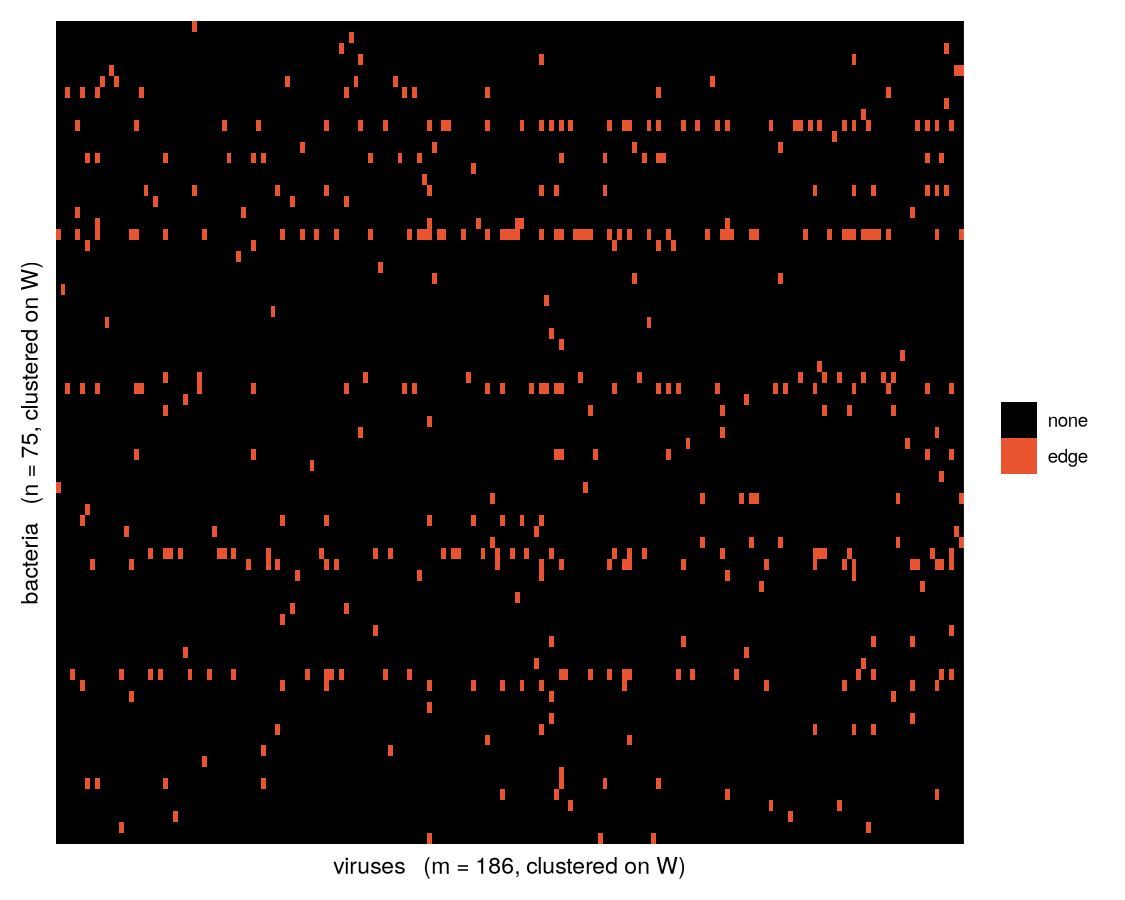
\includegraphics[width=\linewidth]{figures/fig_ap_interaction_Y_matrix_crc.png}
    \caption{CRC}
  \end{subfigure}\hfill
  \begin{subfigure}[t]{0.32\textwidth}
    \centering
    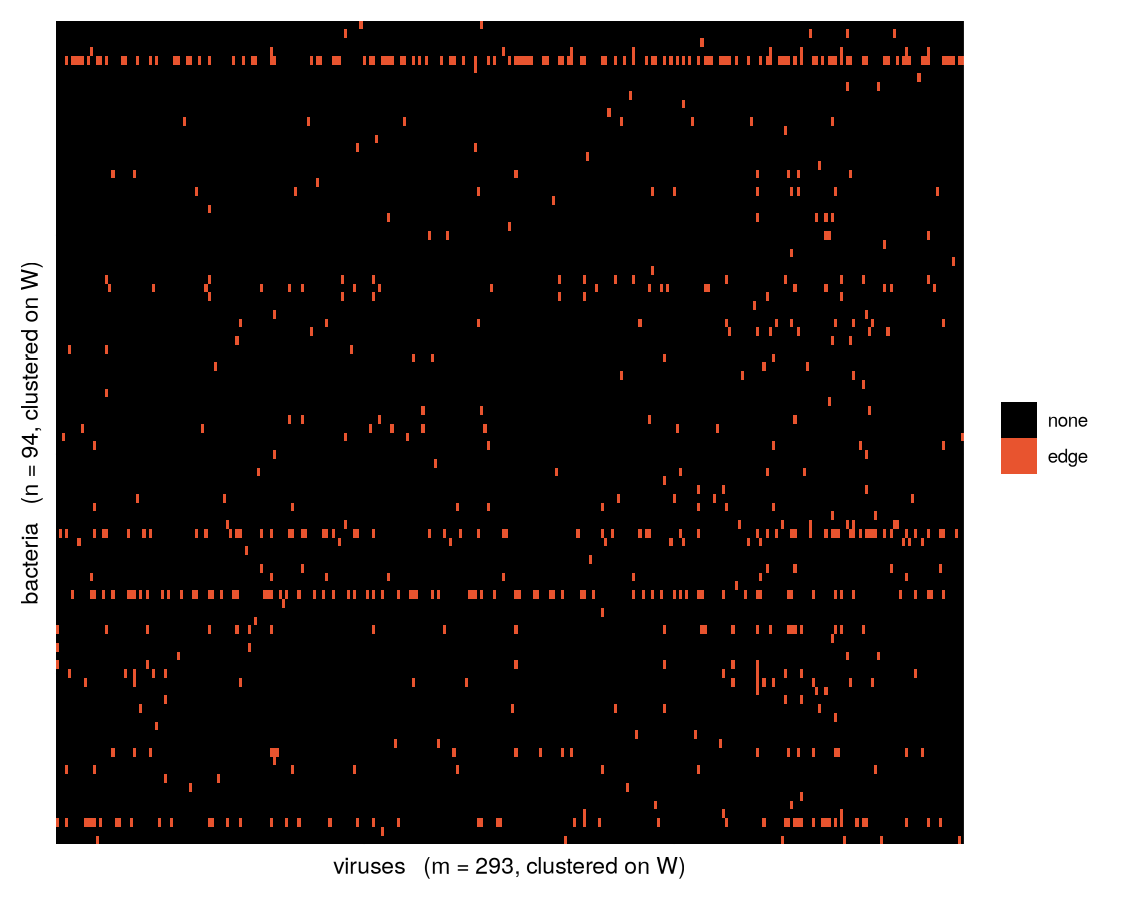
\includegraphics[width=\linewidth]{figures/fig_ap_interaction_Y_matrix_ibd.png}
    \caption{IBD}
  \end{subfigure}\hfill
  \begin{subfigure}[t]{0.32\textwidth}
    \centering
    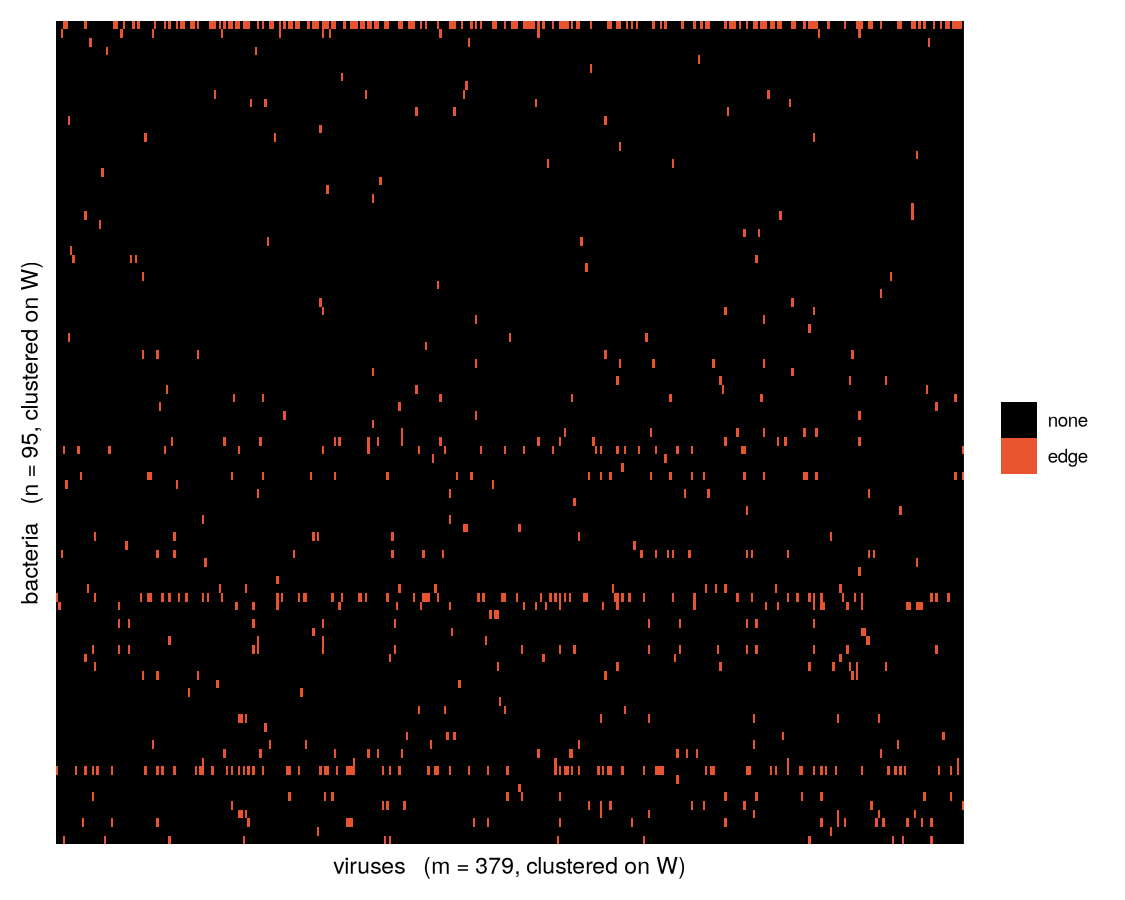
\includegraphics[width=\linewidth]{figures/fig_ap_interaction_Y_matrix_gvhd.png}
    \caption{GvHD}
  \end{subfigure}
  \caption{CRISPR linkage over all candidate pairs}
  \label{fig:ap-ymat}
\end{figure}

\begin{figure}[H]
  \centering
  \begin{subfigure}[t]{0.32\textwidth}
    \centering
    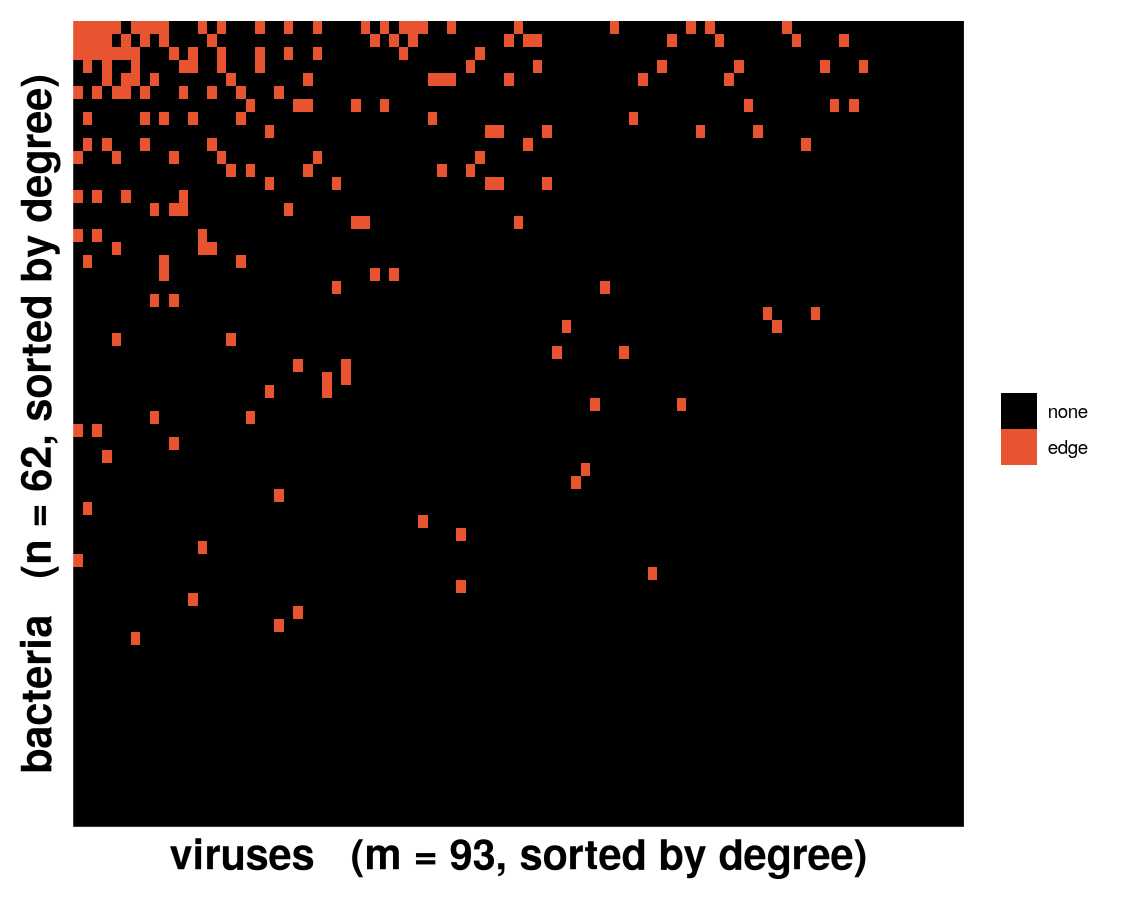
\includegraphics[width=\linewidth]{figures/fig_ap_interaction_Y_matrix_observed_crc.png}
    \caption{CRC}
  \end{subfigure}\hfill
  \begin{subfigure}[t]{0.32\textwidth}
    \centering
    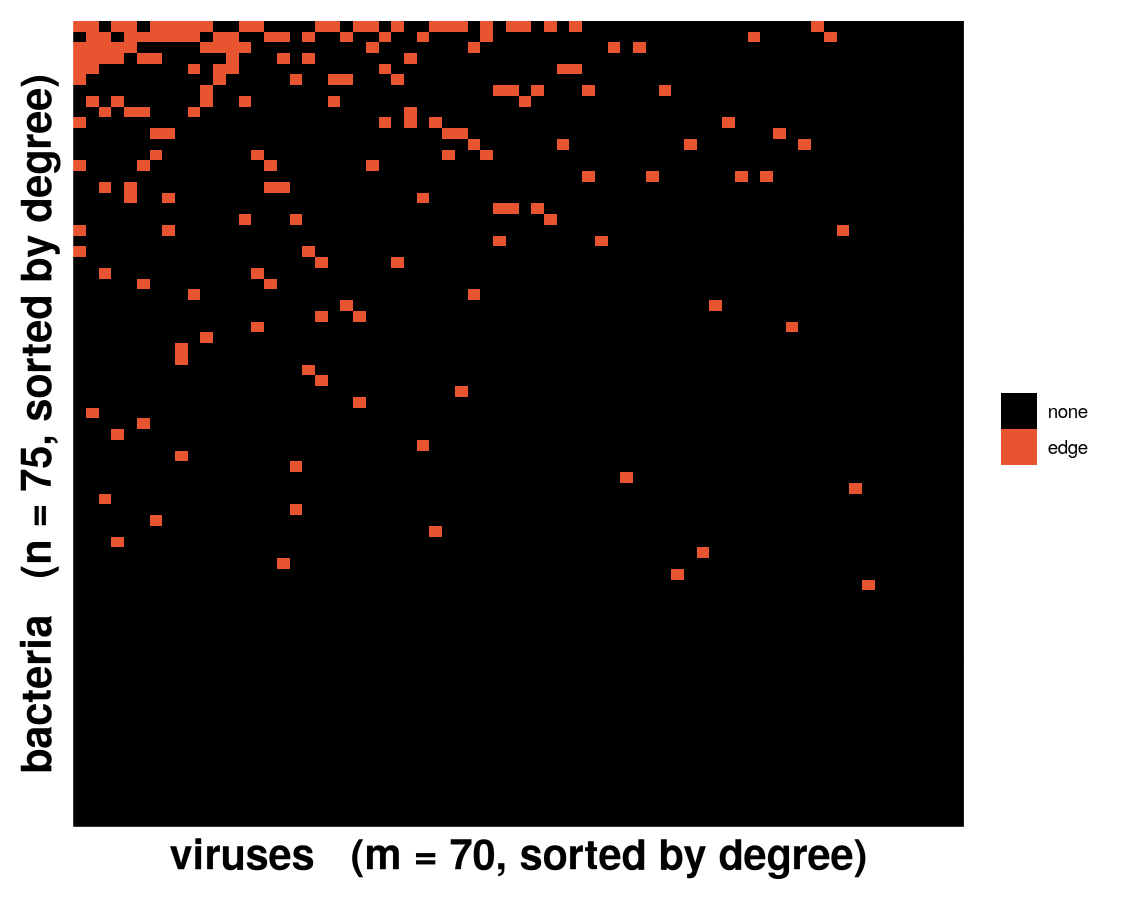
\includegraphics[width=\linewidth]{figures/fig_ap_interaction_Y_matrix_observed_ibd.png}
    \caption{IBD}
  \end{subfigure}\hfill
  \begin{subfigure}[t]{0.32\textwidth}
    \centering
    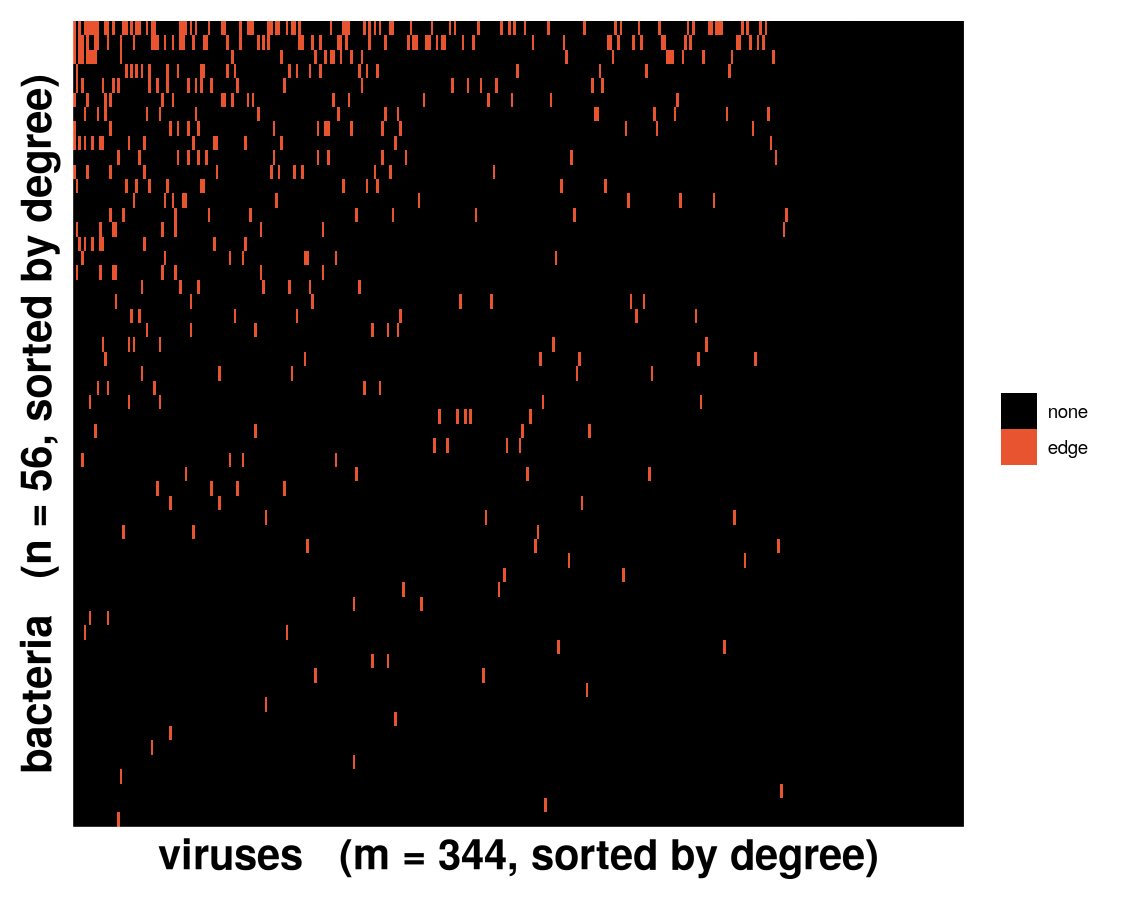
\includegraphics[width=\linewidth]{figures/fig_ap_interaction_Y_matrix_observed_gvhd.png}
    \caption{GvHD}
  \end{subfigure}
  \caption{CRISPR linkage on the observed pairs}
  \label{fig:ap-ymatobs}
\end{figure}

\begin{figure}[H]
  \centering
  \begin{subfigure}[t]{0.32\textwidth}
    \centering
    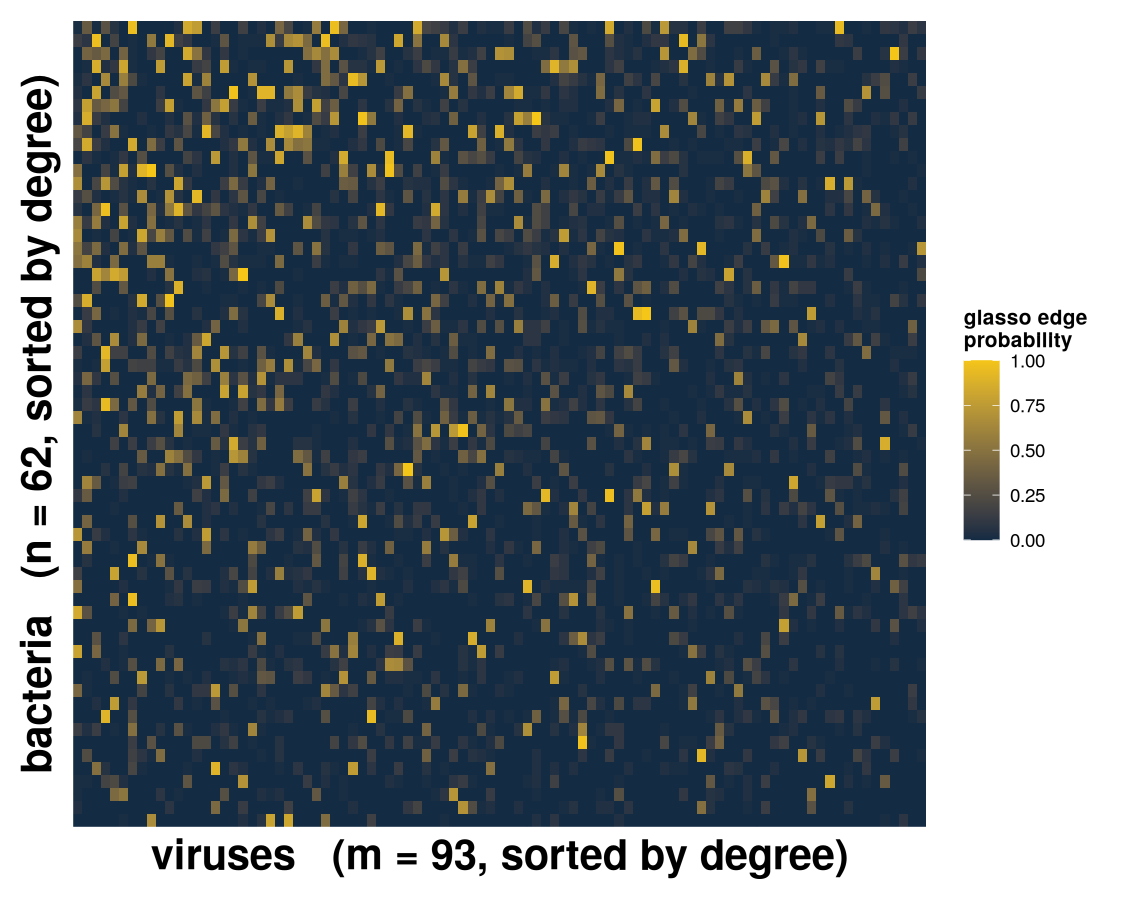
\includegraphics[width=\linewidth]{figures/fig_ap_interaction_W_matrix_observed_crc.png}
    \caption{CRC}
  \end{subfigure}\hfill
  \begin{subfigure}[t]{0.32\textwidth}
    \centering
    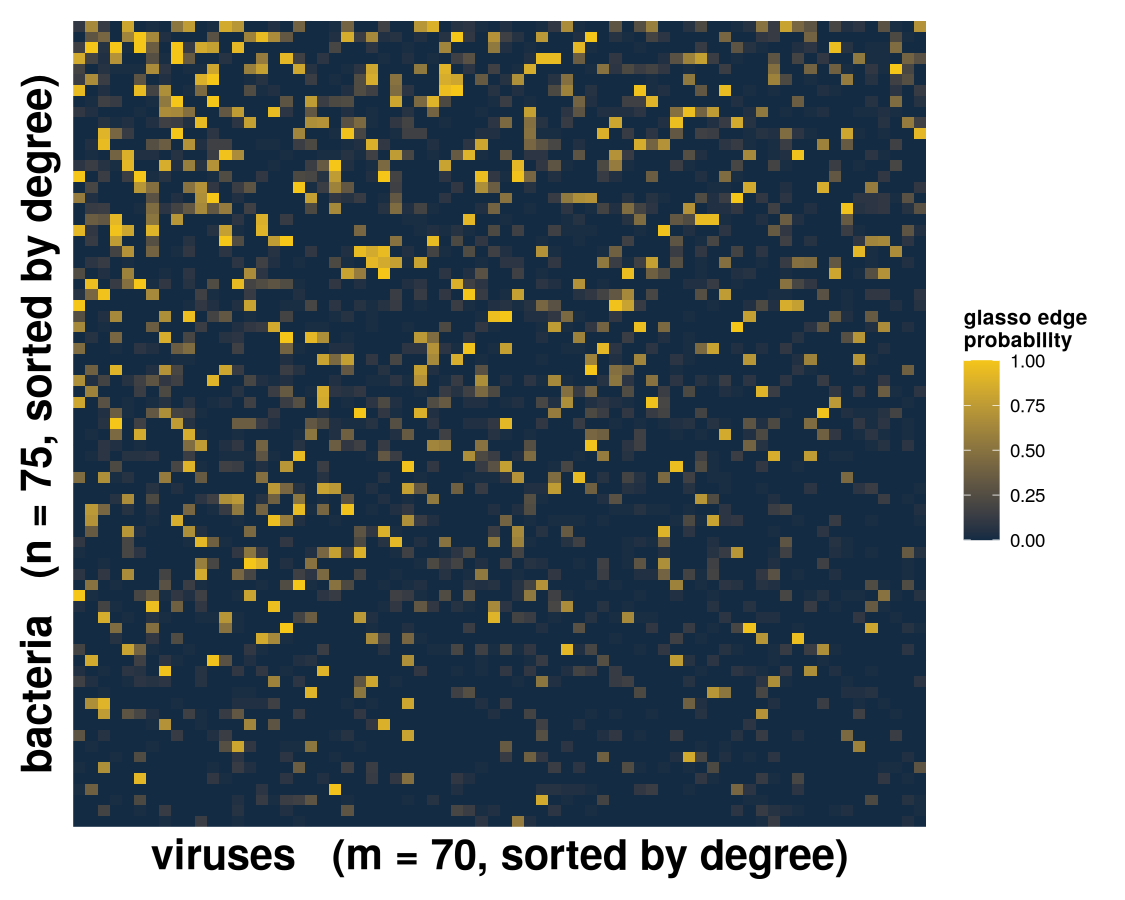
\includegraphics[width=\linewidth]{figures/fig_ap_interaction_W_matrix_observed_ibd.png}
    \caption{IBD}
  \end{subfigure}\hfill
  \begin{subfigure}[t]{0.32\textwidth}
    \centering
    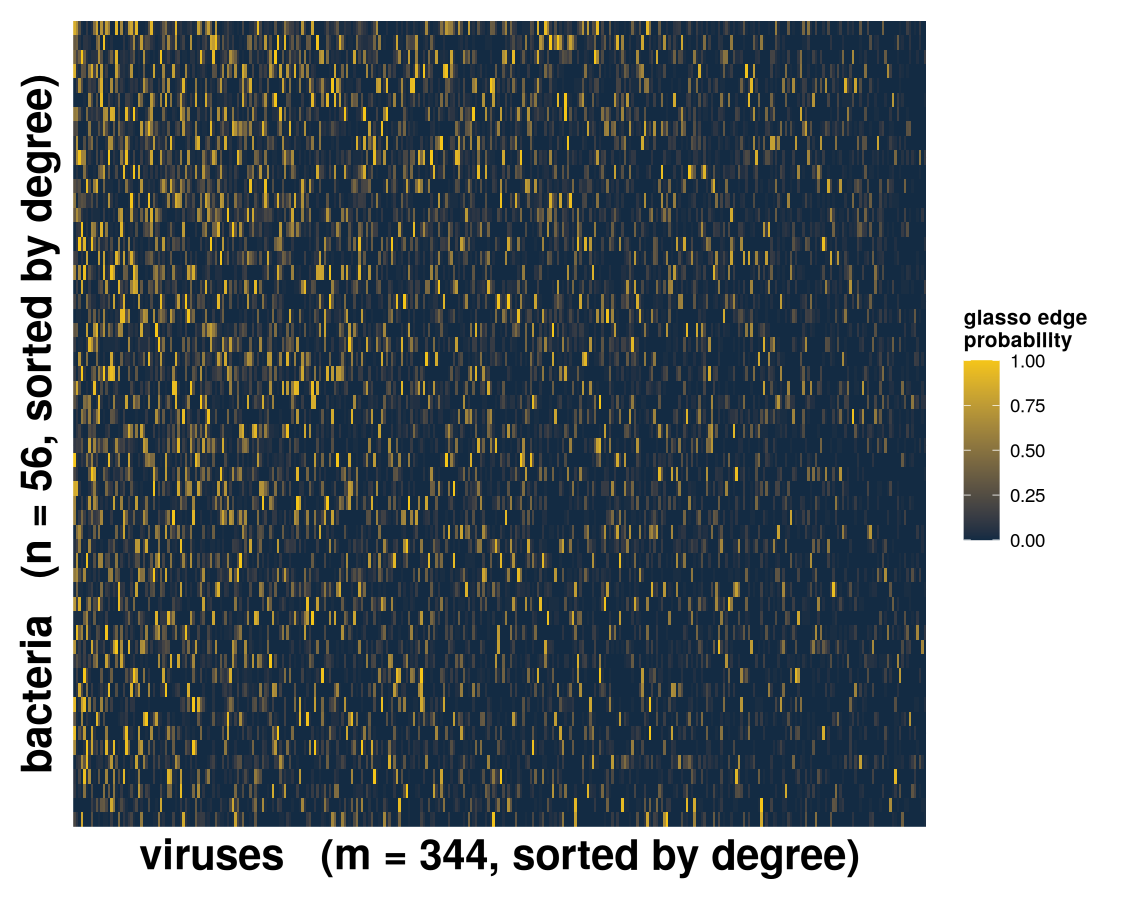
\includegraphics[width=\linewidth]{figures/fig_ap_interaction_W_matrix_observed_gvhd.png}
    \caption{GvHD}
  \end{subfigure}
  \caption{Edge selection probability on the observed pairs}
  \label{fig:ap-wmatobs}
\end{figure}

\begin{figure}[H]
  \centering
  \begin{subfigure}[t]{0.32\textwidth}
    \centering
    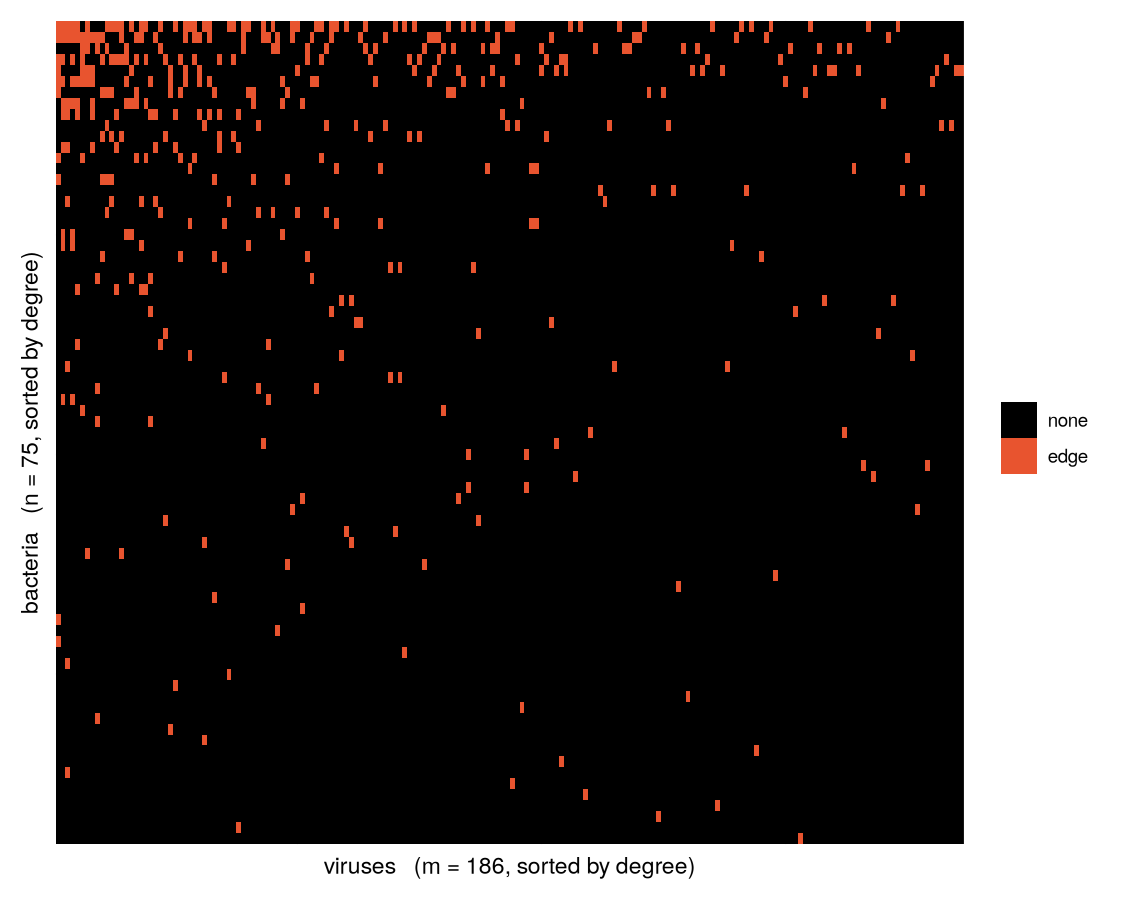
\includegraphics[width=\linewidth]{figures/fig_ap_nestedness_Y_crc.png}
    \caption{CRC}
  \end{subfigure}\hfill
  \begin{subfigure}[t]{0.32\textwidth}
    \centering
    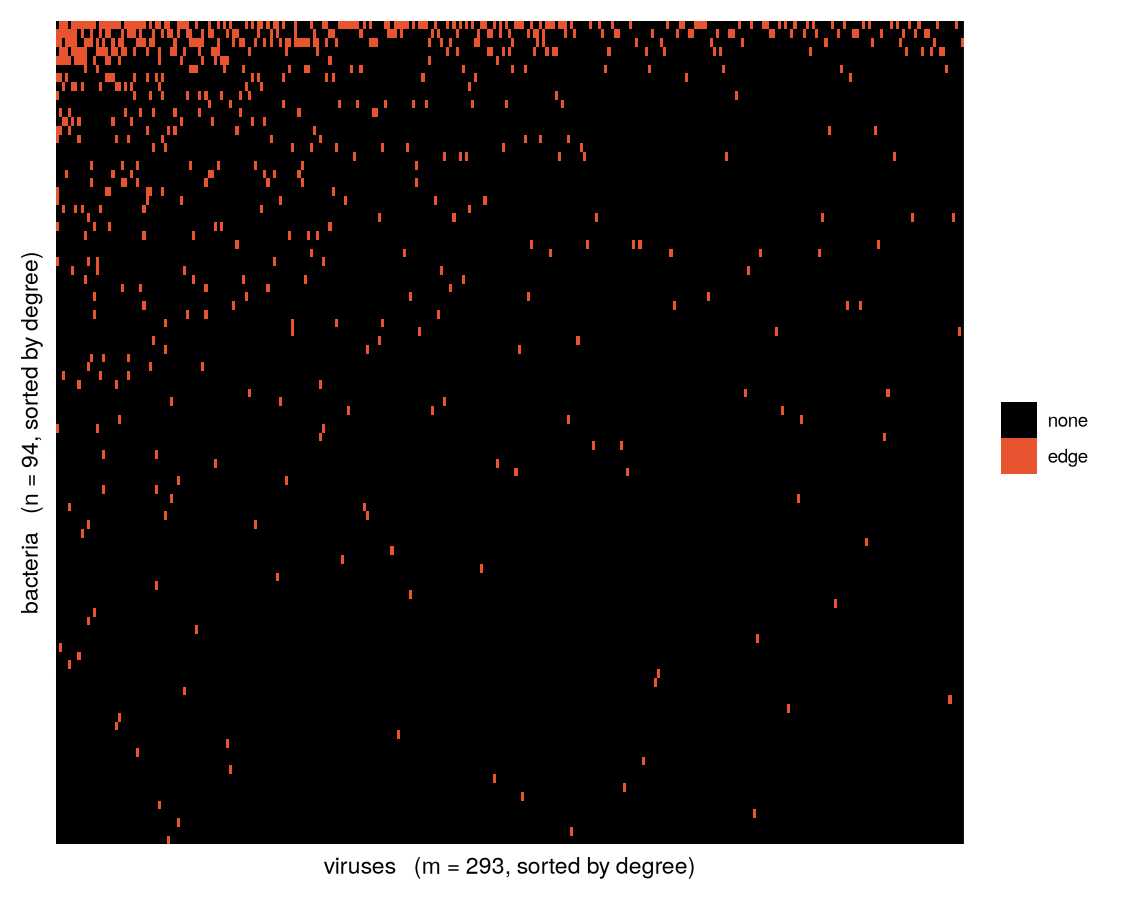
\includegraphics[width=\linewidth]{figures/fig_ap_nestedness_Y_ibd.png}
    \caption{IBD}
  \end{subfigure}\hfill
  \begin{subfigure}[t]{0.32\textwidth}
    \centering
    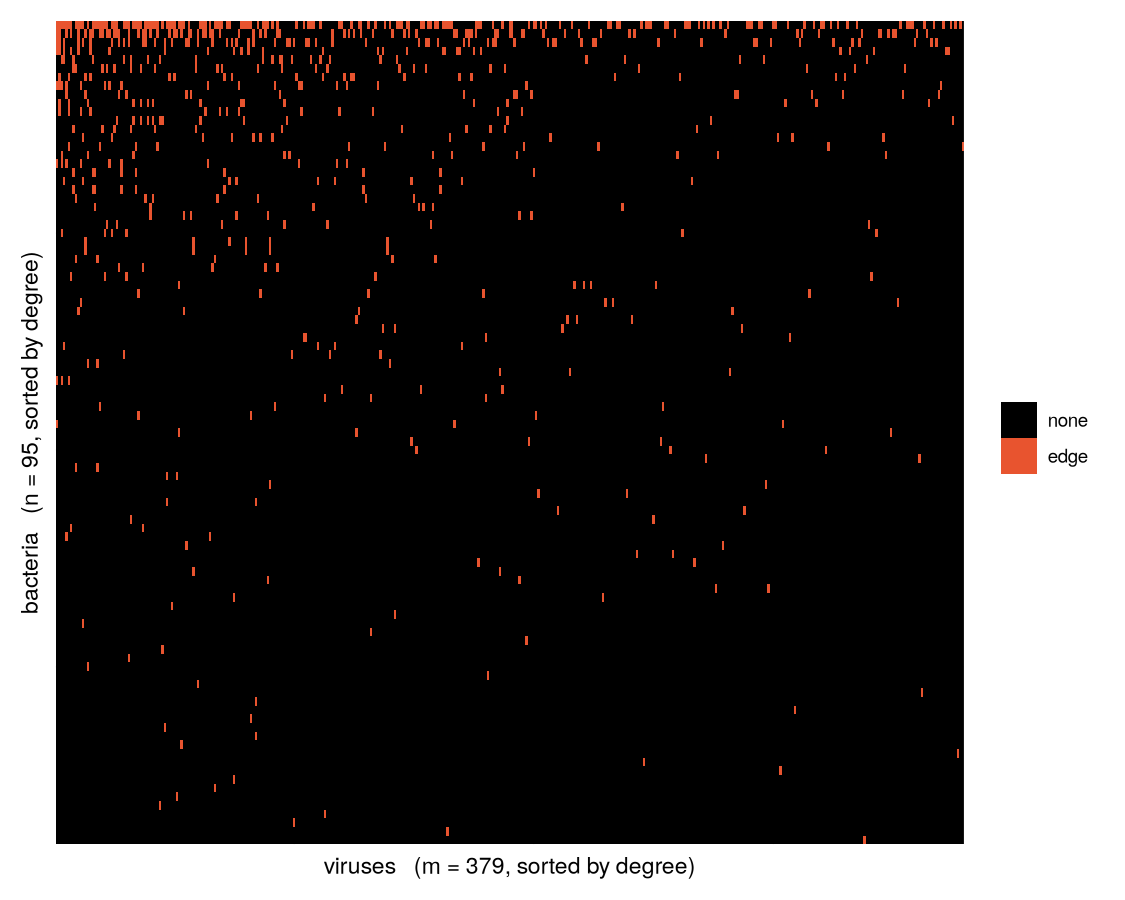
\includegraphics[width=\linewidth]{figures/fig_ap_nestedness_Y_gvhd.png}
    \caption{GvHD}
  \end{subfigure}
  \caption{Nestedness of the CRISPR linkage}
  \label{fig:ap-nesty}
\end{figure}

\begin{figure}[H]
  \centering
  \begin{subfigure}[t]{0.32\textwidth}
    \centering
    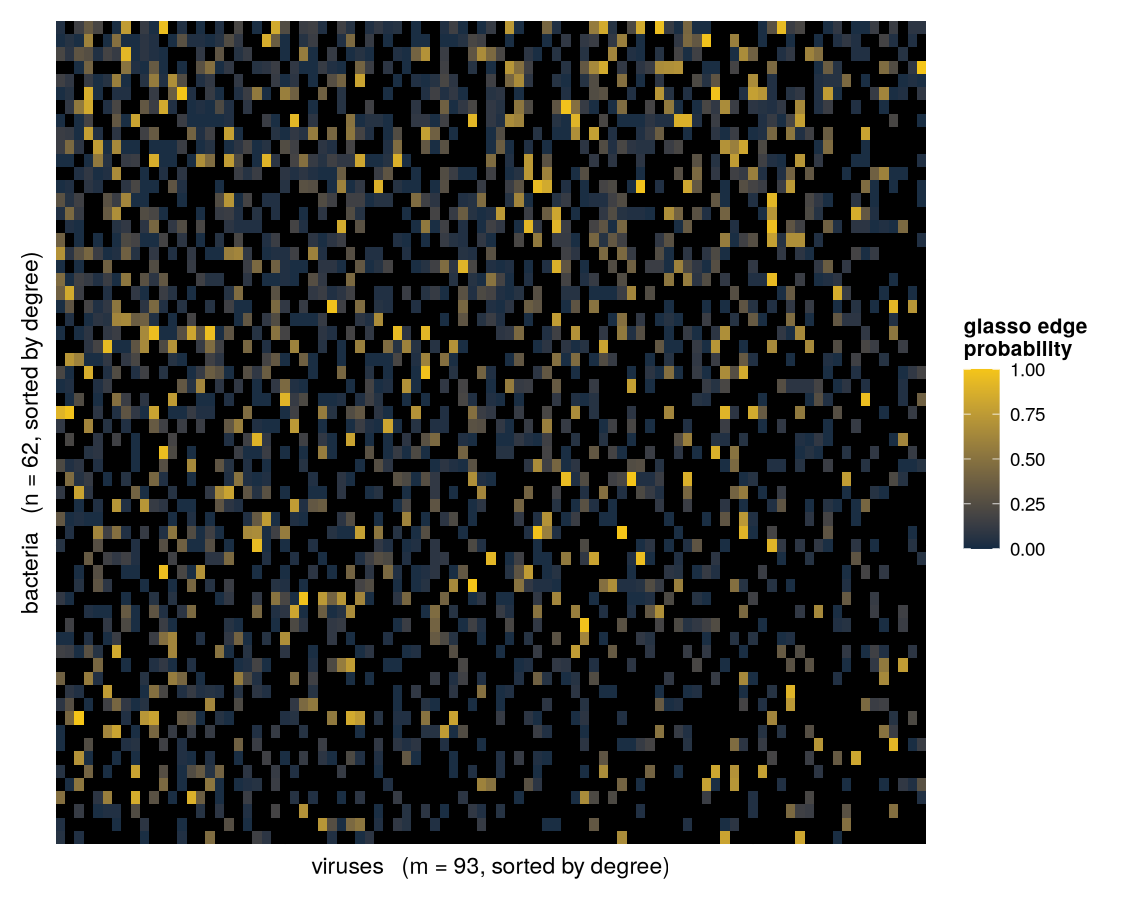
\includegraphics[width=\linewidth]{figures/fig_ap_nestedness_W_crc.png}
    \caption{CRC}
  \end{subfigure}\hfill
  \begin{subfigure}[t]{0.32\textwidth}
    \centering
    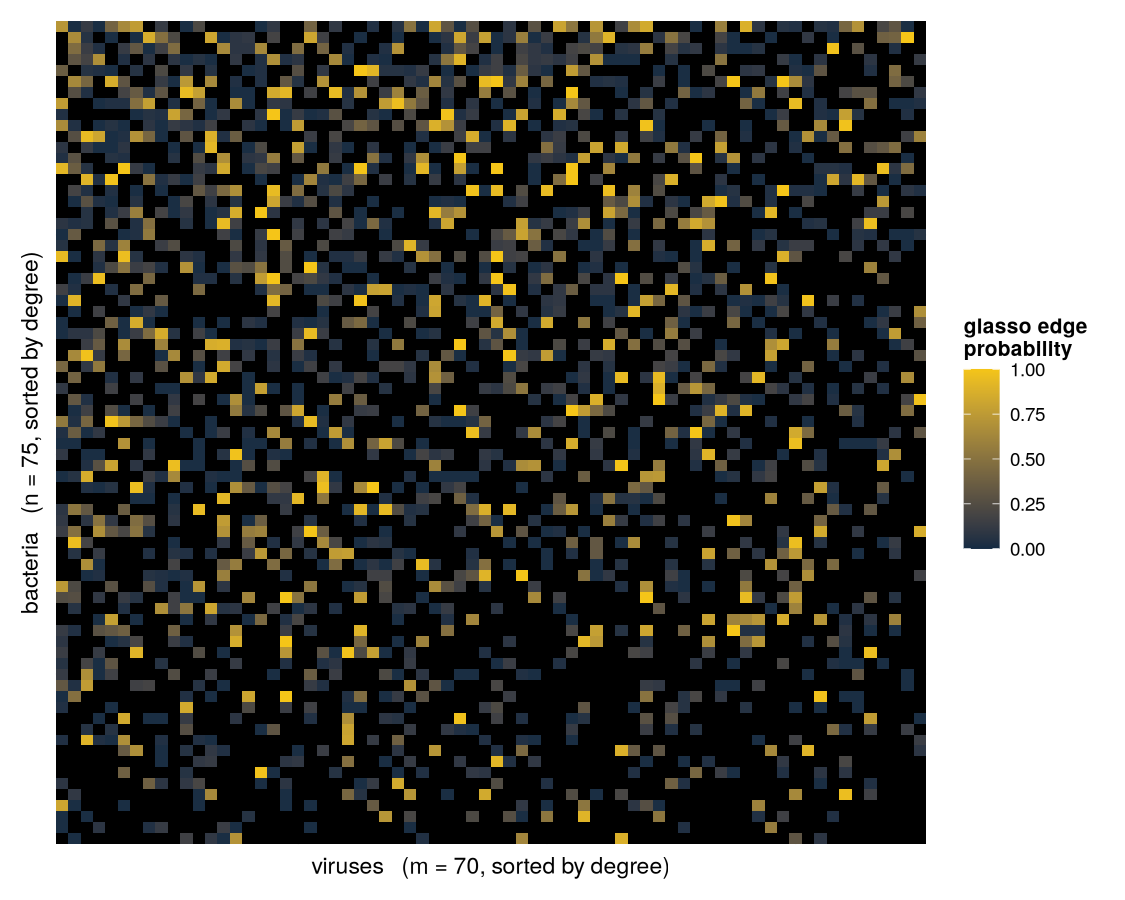
\includegraphics[width=\linewidth]{figures/fig_ap_nestedness_W_ibd.png}
    \caption{IBD}
  \end{subfigure}\hfill
  \begin{subfigure}[t]{0.32\textwidth}
    \centering
    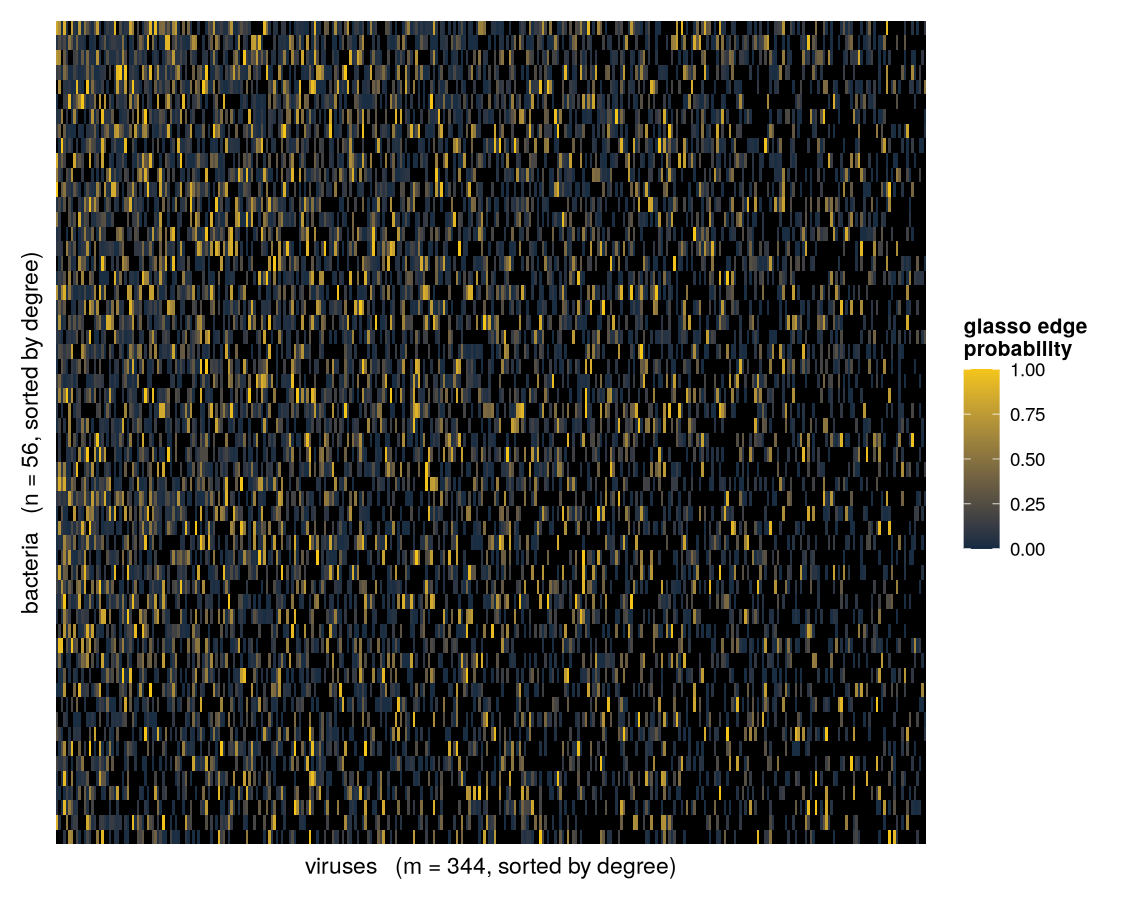
\includegraphics[width=\linewidth]{figures/fig_ap_nestedness_W_gvhd.png}
    \caption{GvHD}
  \end{subfigure}
  \caption{Nestedness of the edge selection probability}
  \label{fig:ap-nestw}
\end{figure}

\subsection{Test Scores by Model}

\begin{figure}[H]
  \centering
  \begin{subfigure}[t]{0.32\textwidth}
    \centering
    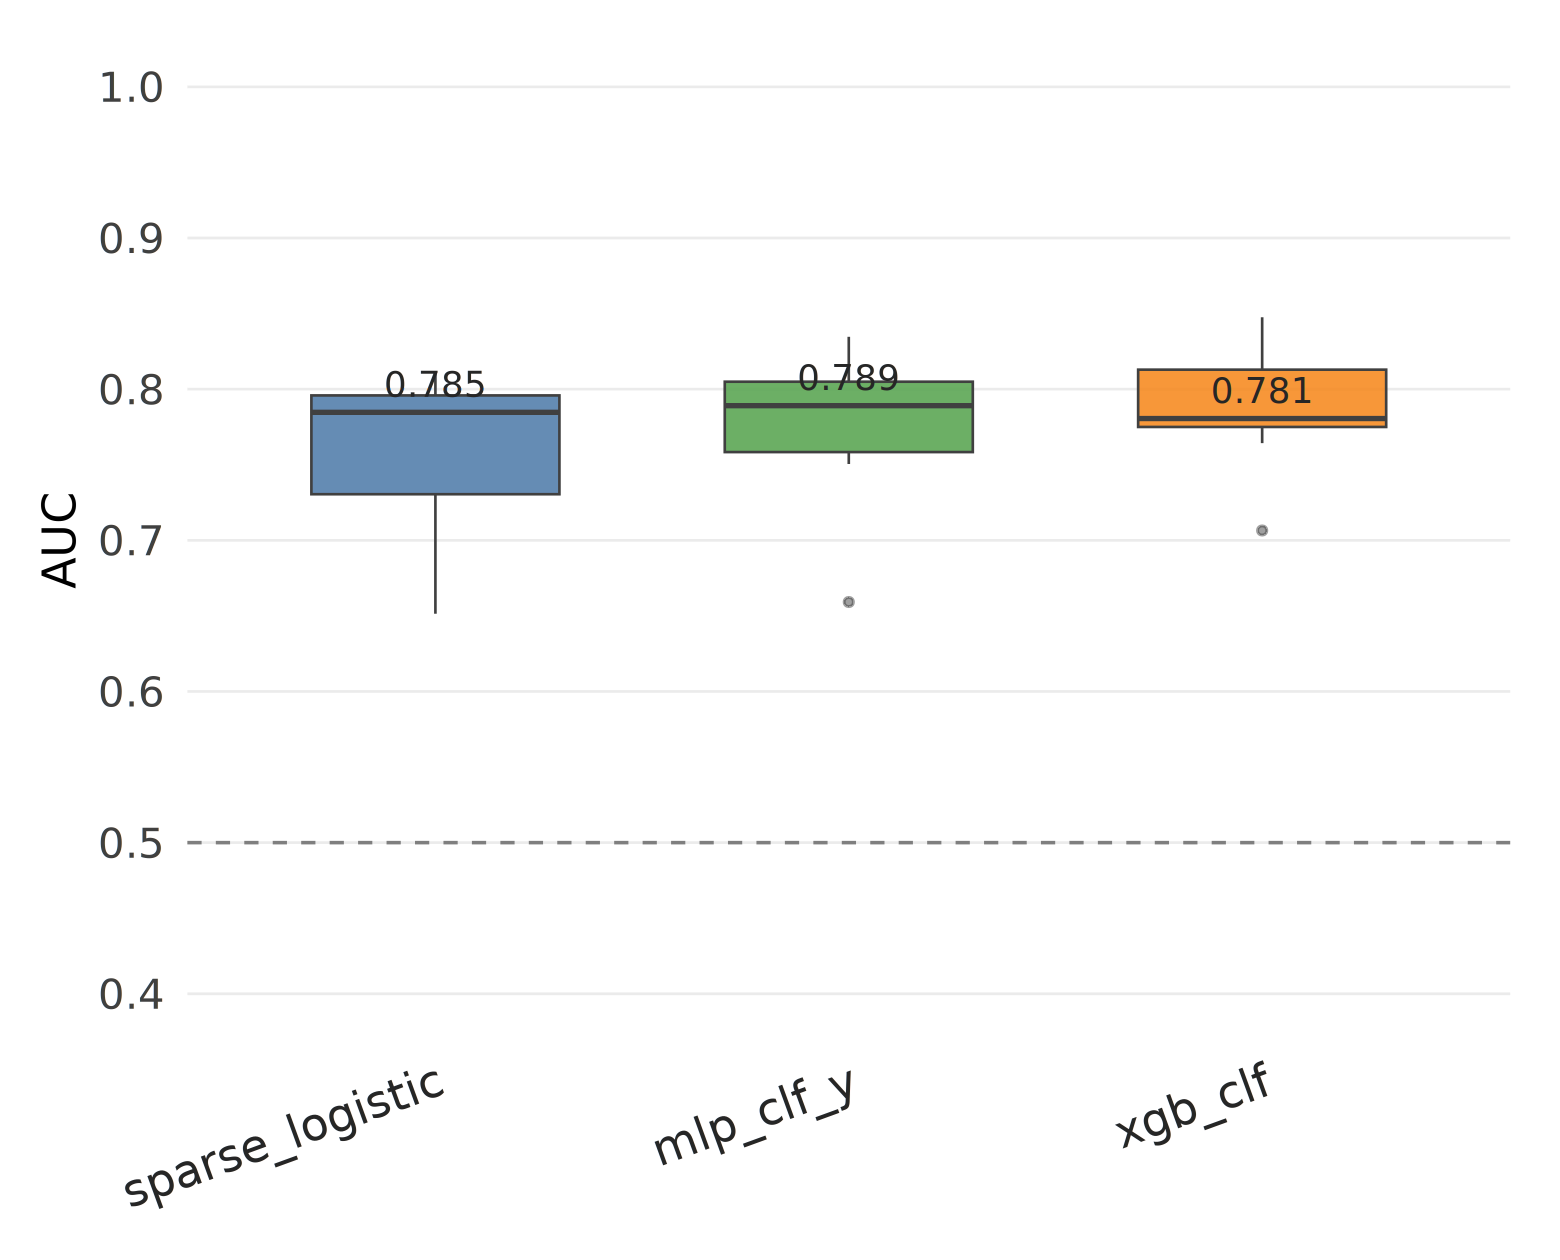
\includegraphics[width=\linewidth]{figures/fig_ap_y_auc_baseline_crc.png}
    \caption{CRC}
  \end{subfigure}\hfill
  \begin{subfigure}[t]{0.32\textwidth}
    \centering
    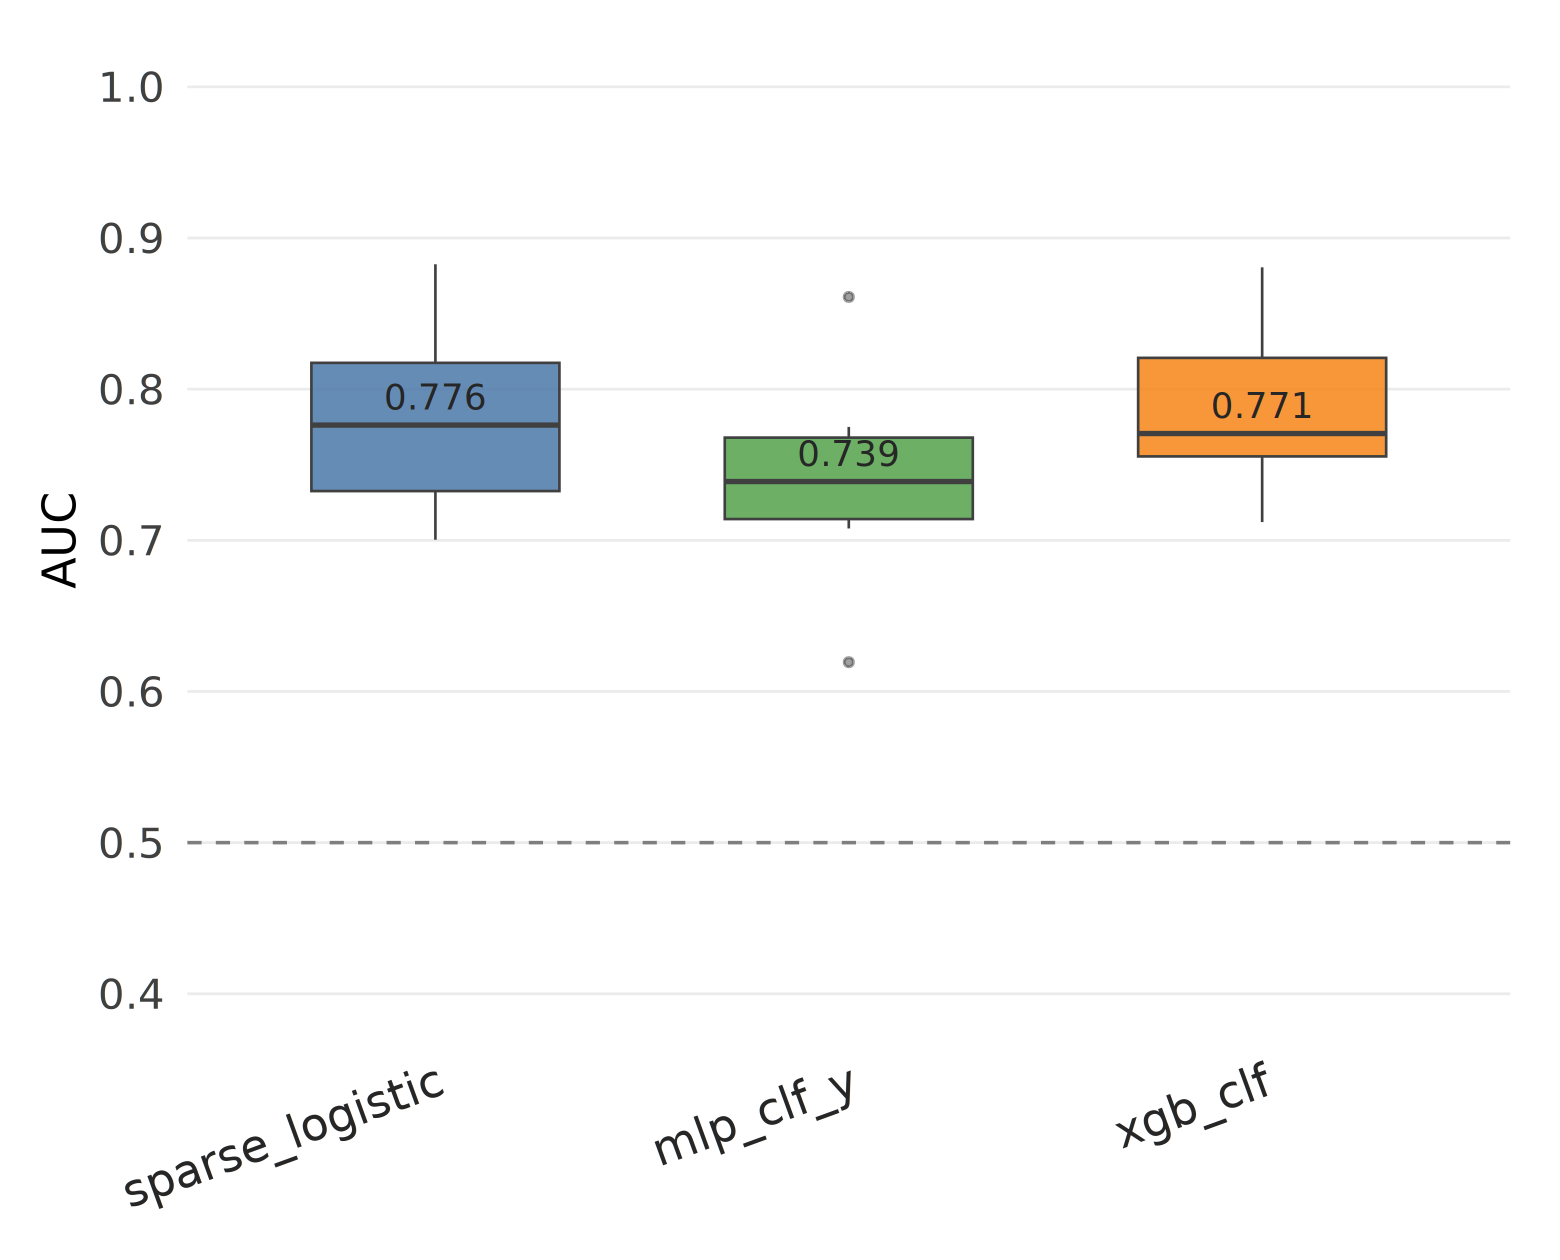
\includegraphics[width=\linewidth]{figures/fig_ap_y_auc_baseline_ibd.png}
    \caption{IBD}
  \end{subfigure}\hfill
  \begin{subfigure}[t]{0.32\textwidth}
    \centering
    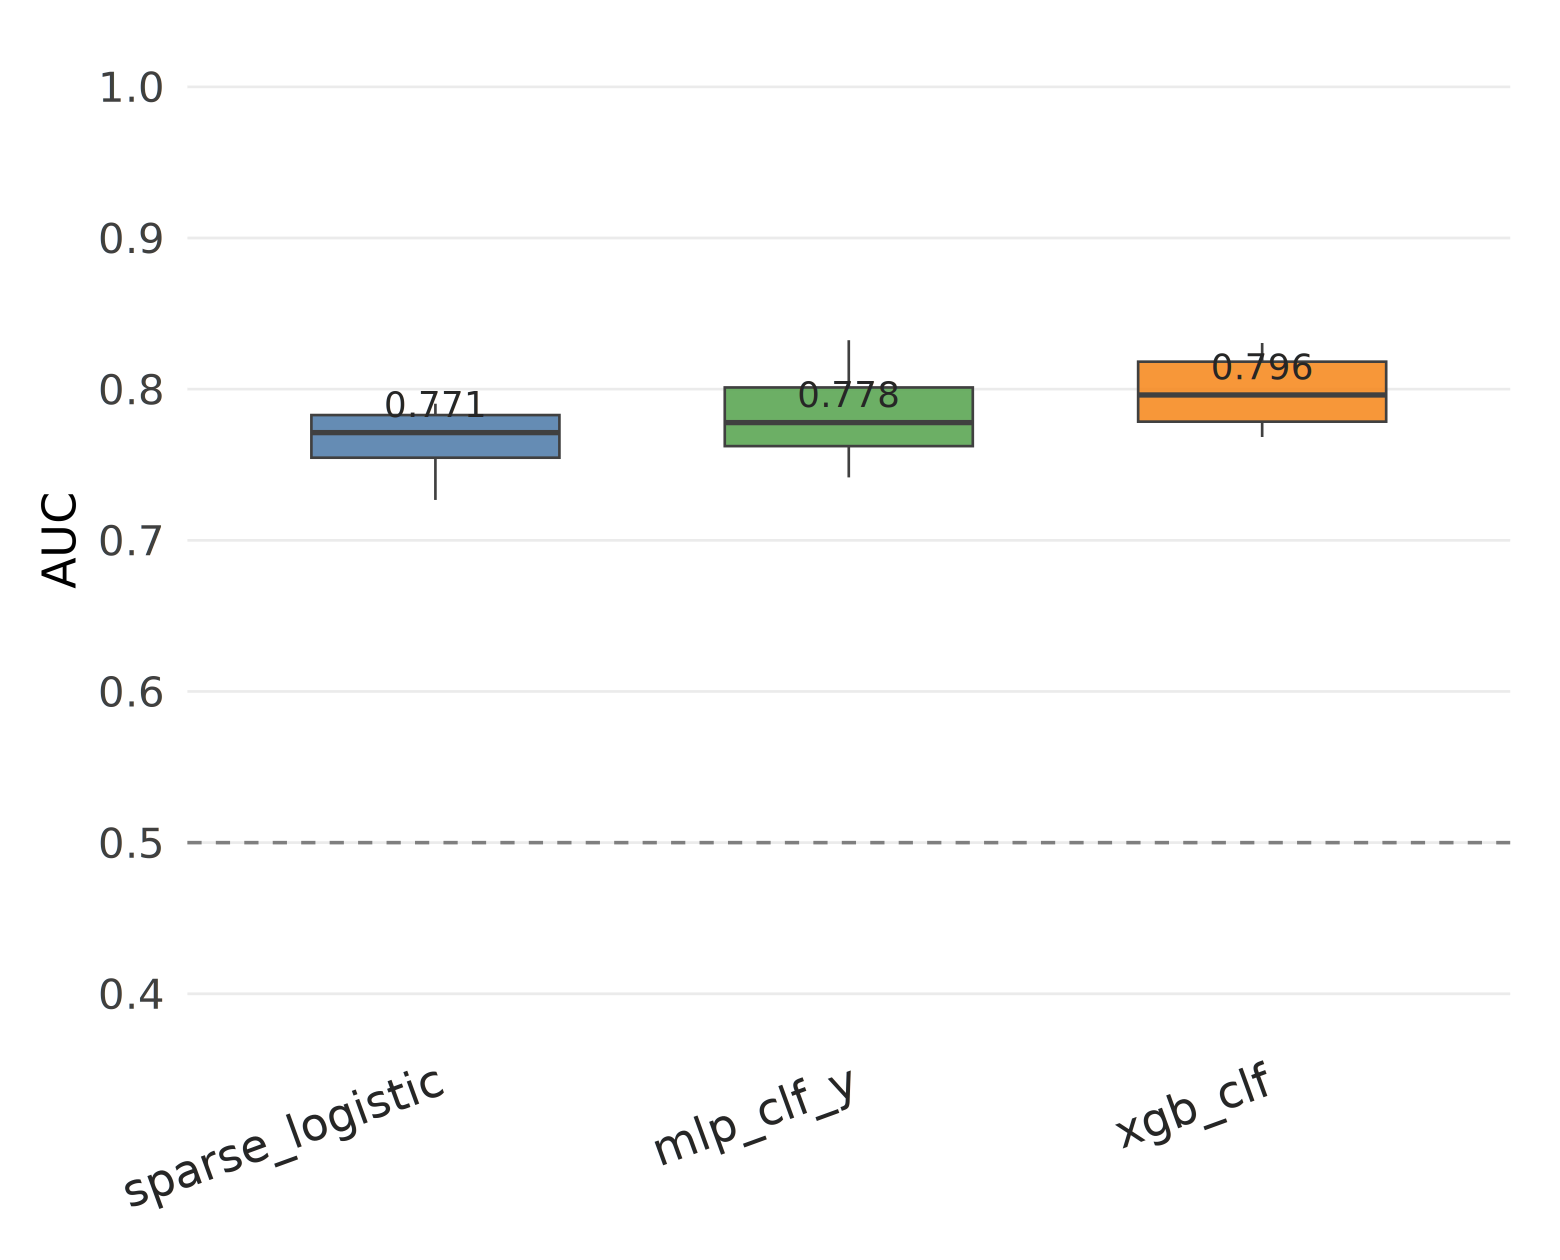
\includegraphics[width=\linewidth]{figures/fig_ap_y_auc_baseline_gvhd.png}
    \caption{GvHD}
  \end{subfigure}
  \caption{Test AUC on CRISPR linkage, baseline models}
  \label{fig:ap-yaucb}
\end{figure}

\begin{figure}[H]
  \centering
  \begin{subfigure}[t]{0.32\textwidth}
    \centering
    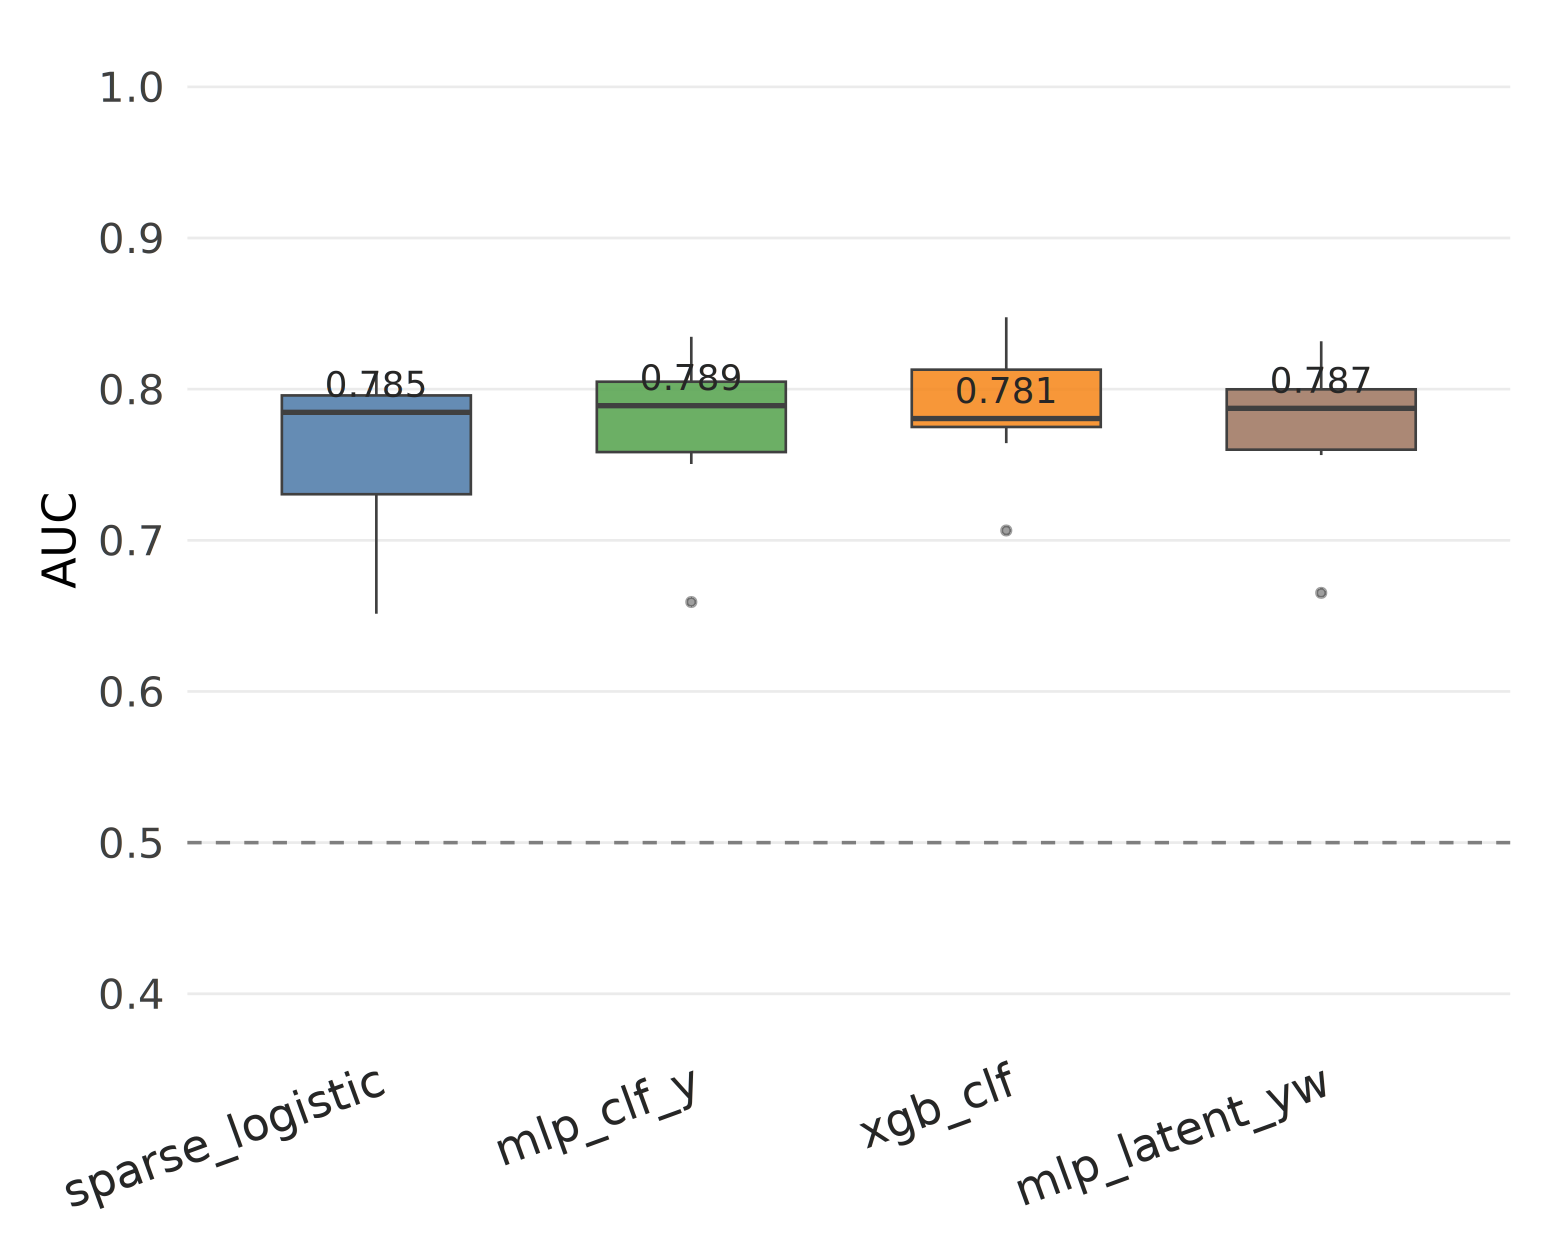
\includegraphics[width=\linewidth]{figures/fig_ap_y_auc_all_crc.png}
    \caption{CRC}
  \end{subfigure}\hfill
  \begin{subfigure}[t]{0.32\textwidth}
    \centering
    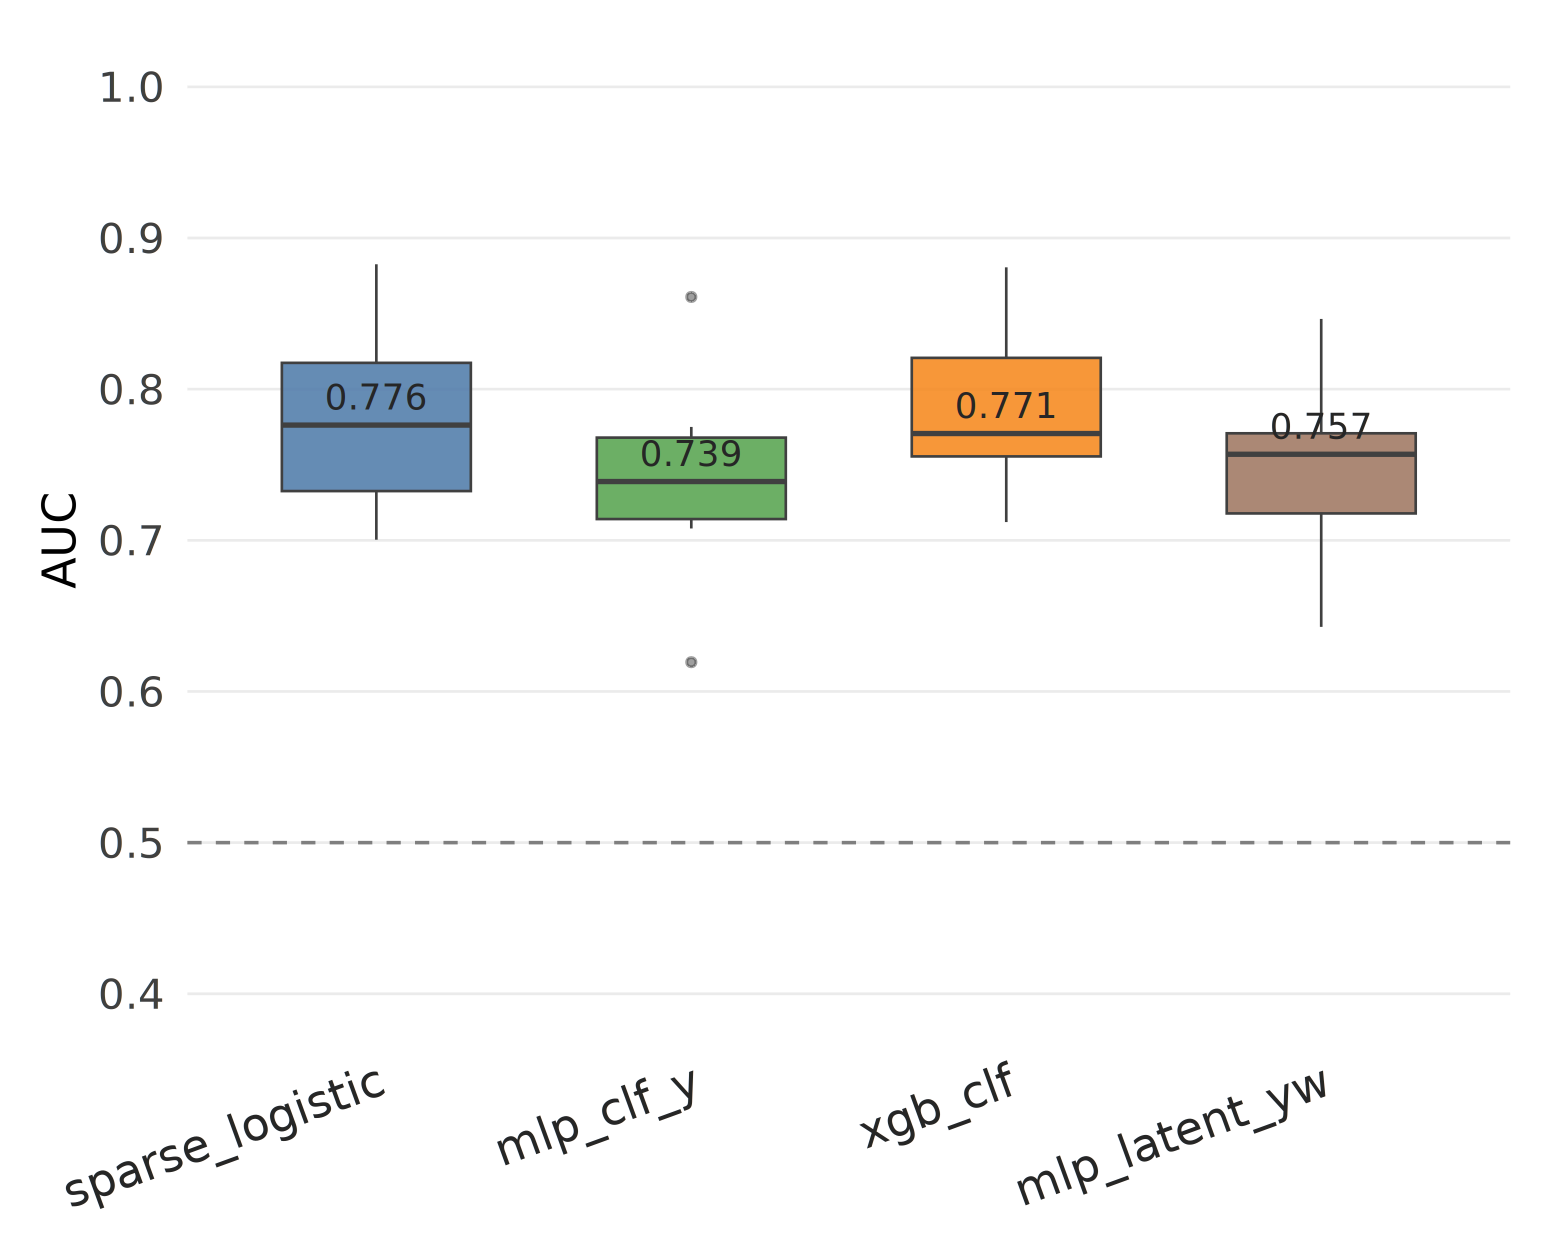
\includegraphics[width=\linewidth]{figures/fig_ap_y_auc_all_ibd.png}
    \caption{IBD}
  \end{subfigure}\hfill
  \begin{subfigure}[t]{0.32\textwidth}
    \centering
    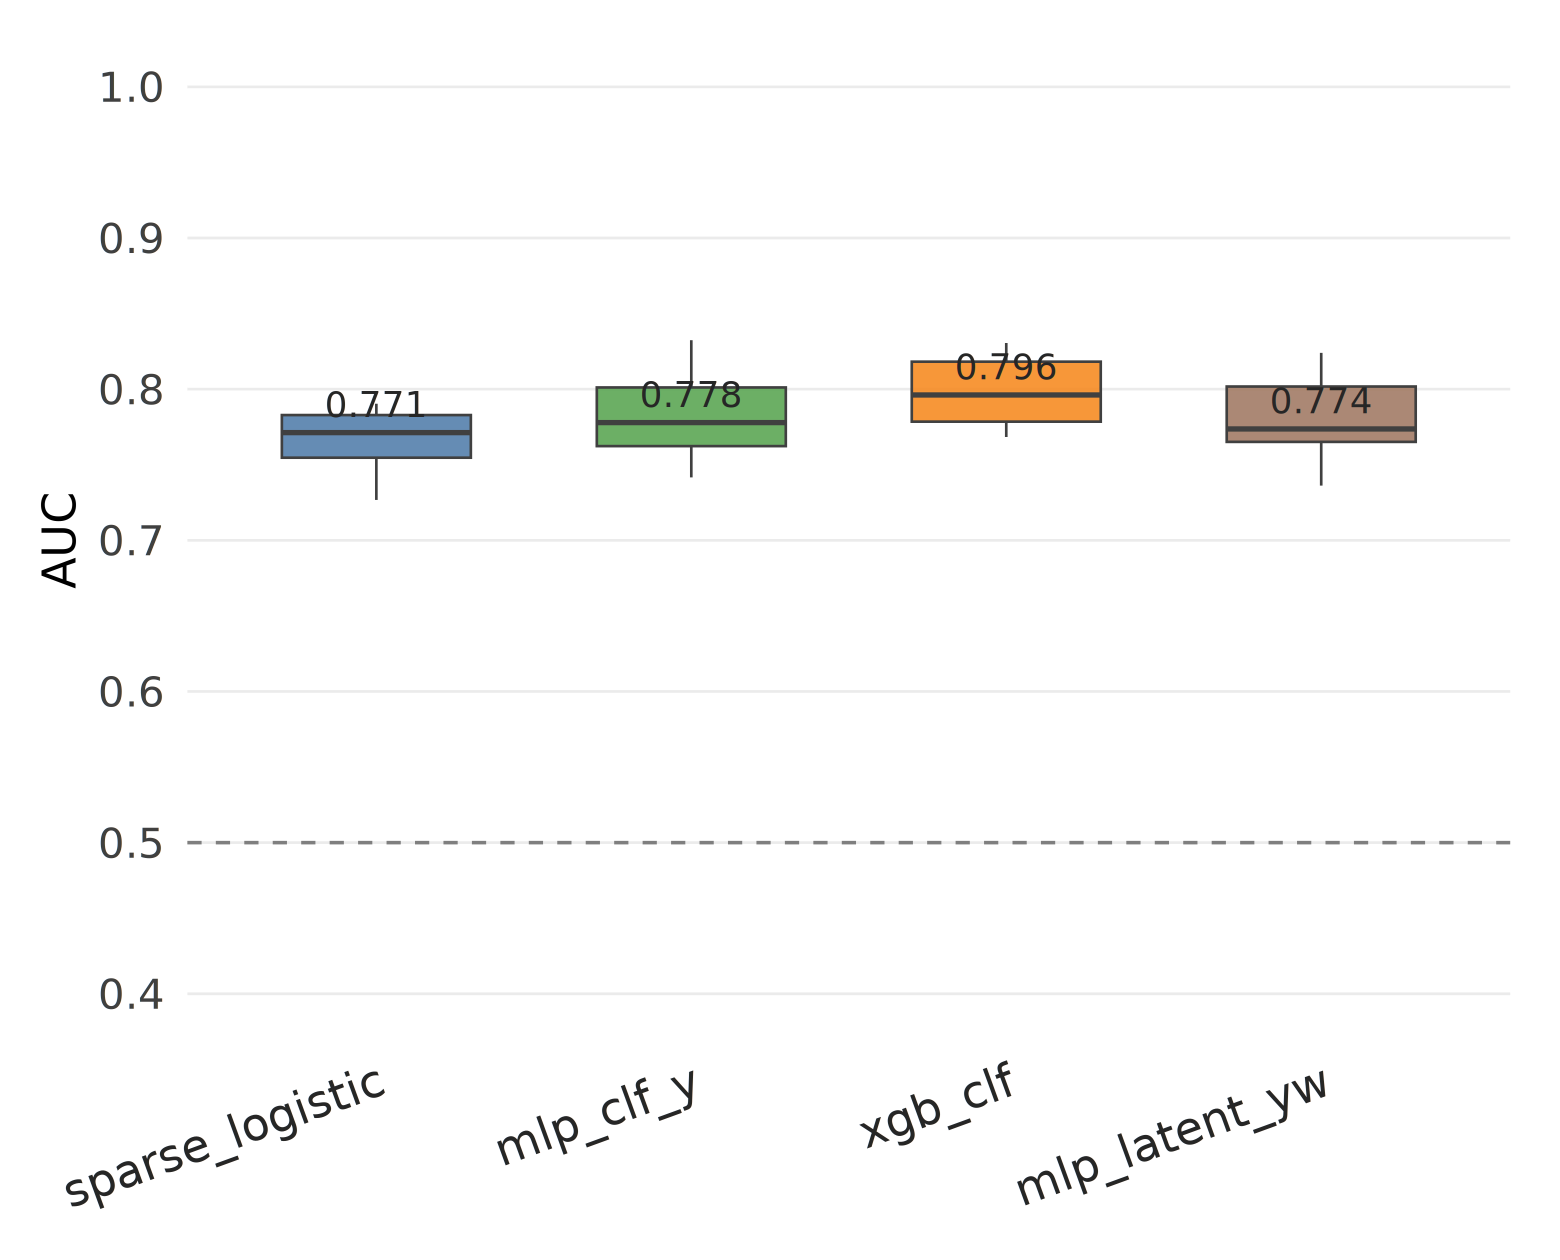
\includegraphics[width=\linewidth]{figures/fig_ap_y_auc_all_gvhd.png}
    \caption{GvHD}
  \end{subfigure}
  \caption{Test AUC on CRISPR linkage, all models}
  \label{fig:ap-yauca}
\end{figure}

\begin{figure}[H]
  \centering
  \begin{subfigure}[t]{0.32\textwidth}
    \centering
    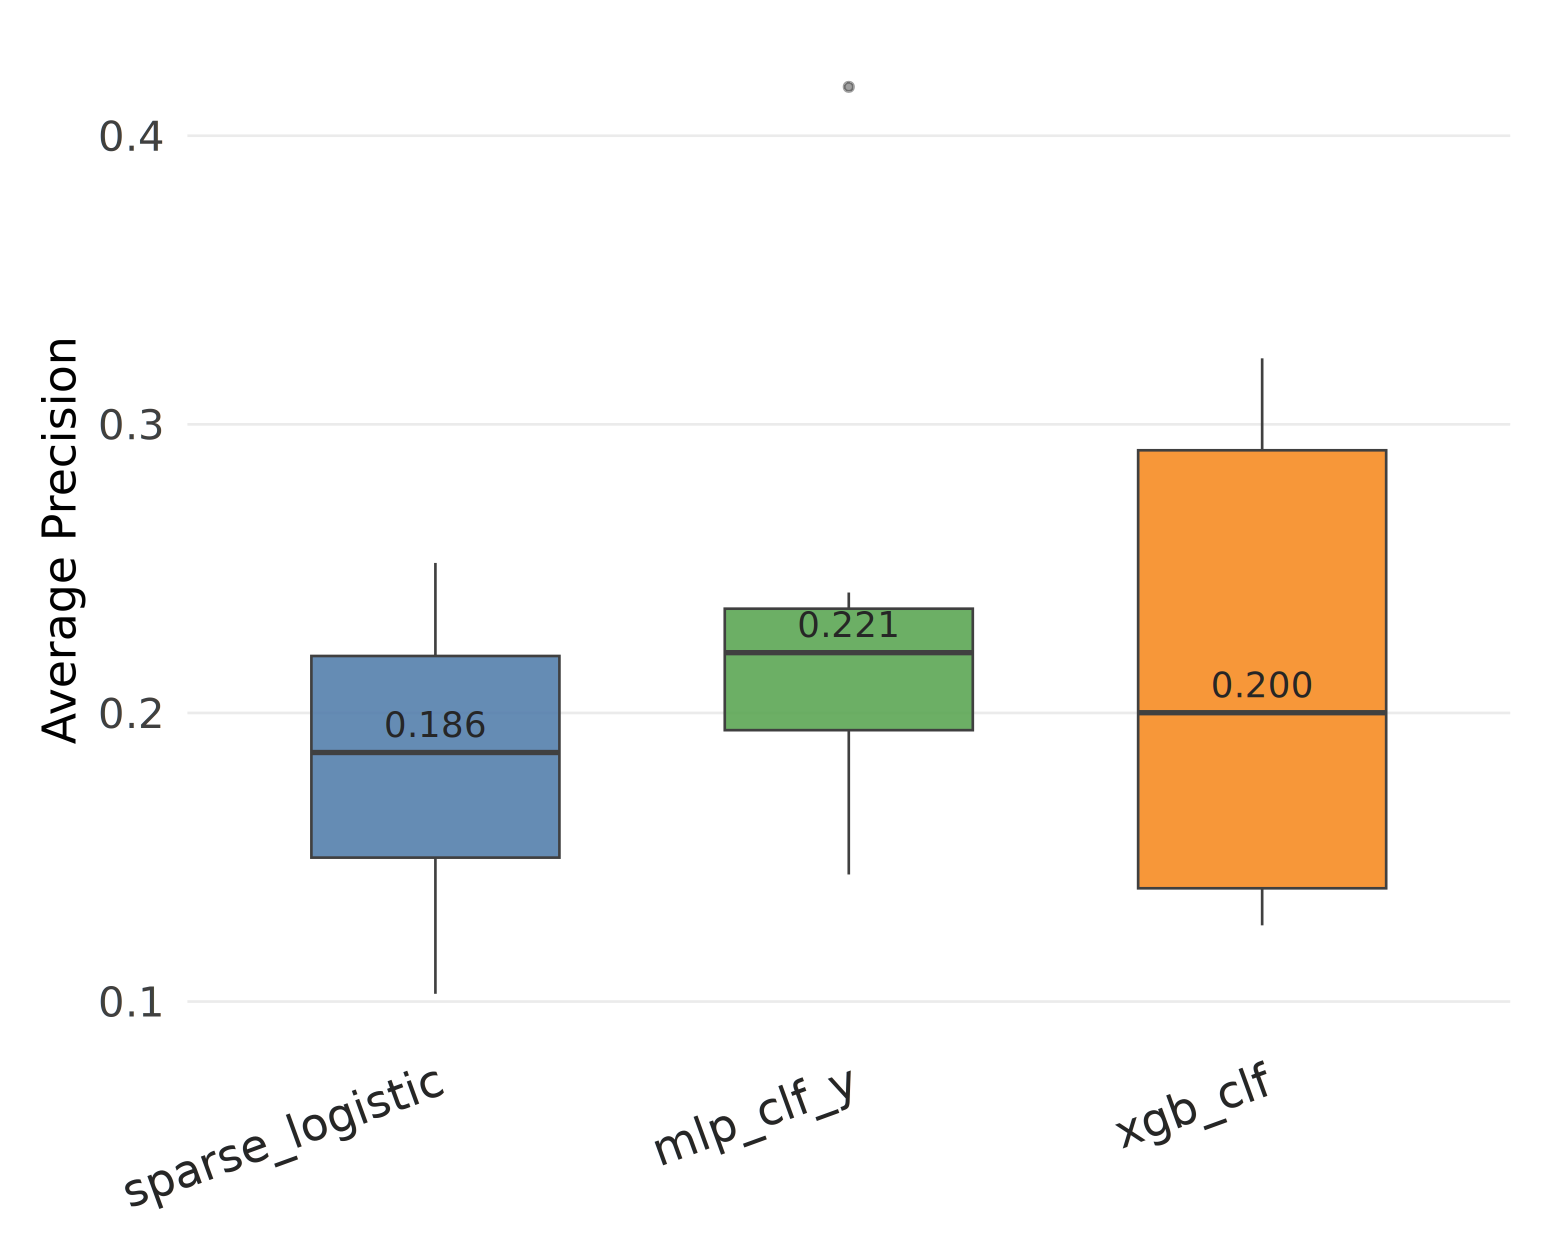
\includegraphics[width=\linewidth]{figures/fig_ap_y_ap_baseline_crc.png}
    \caption{CRC}
  \end{subfigure}\hfill
  \begin{subfigure}[t]{0.32\textwidth}
    \centering
    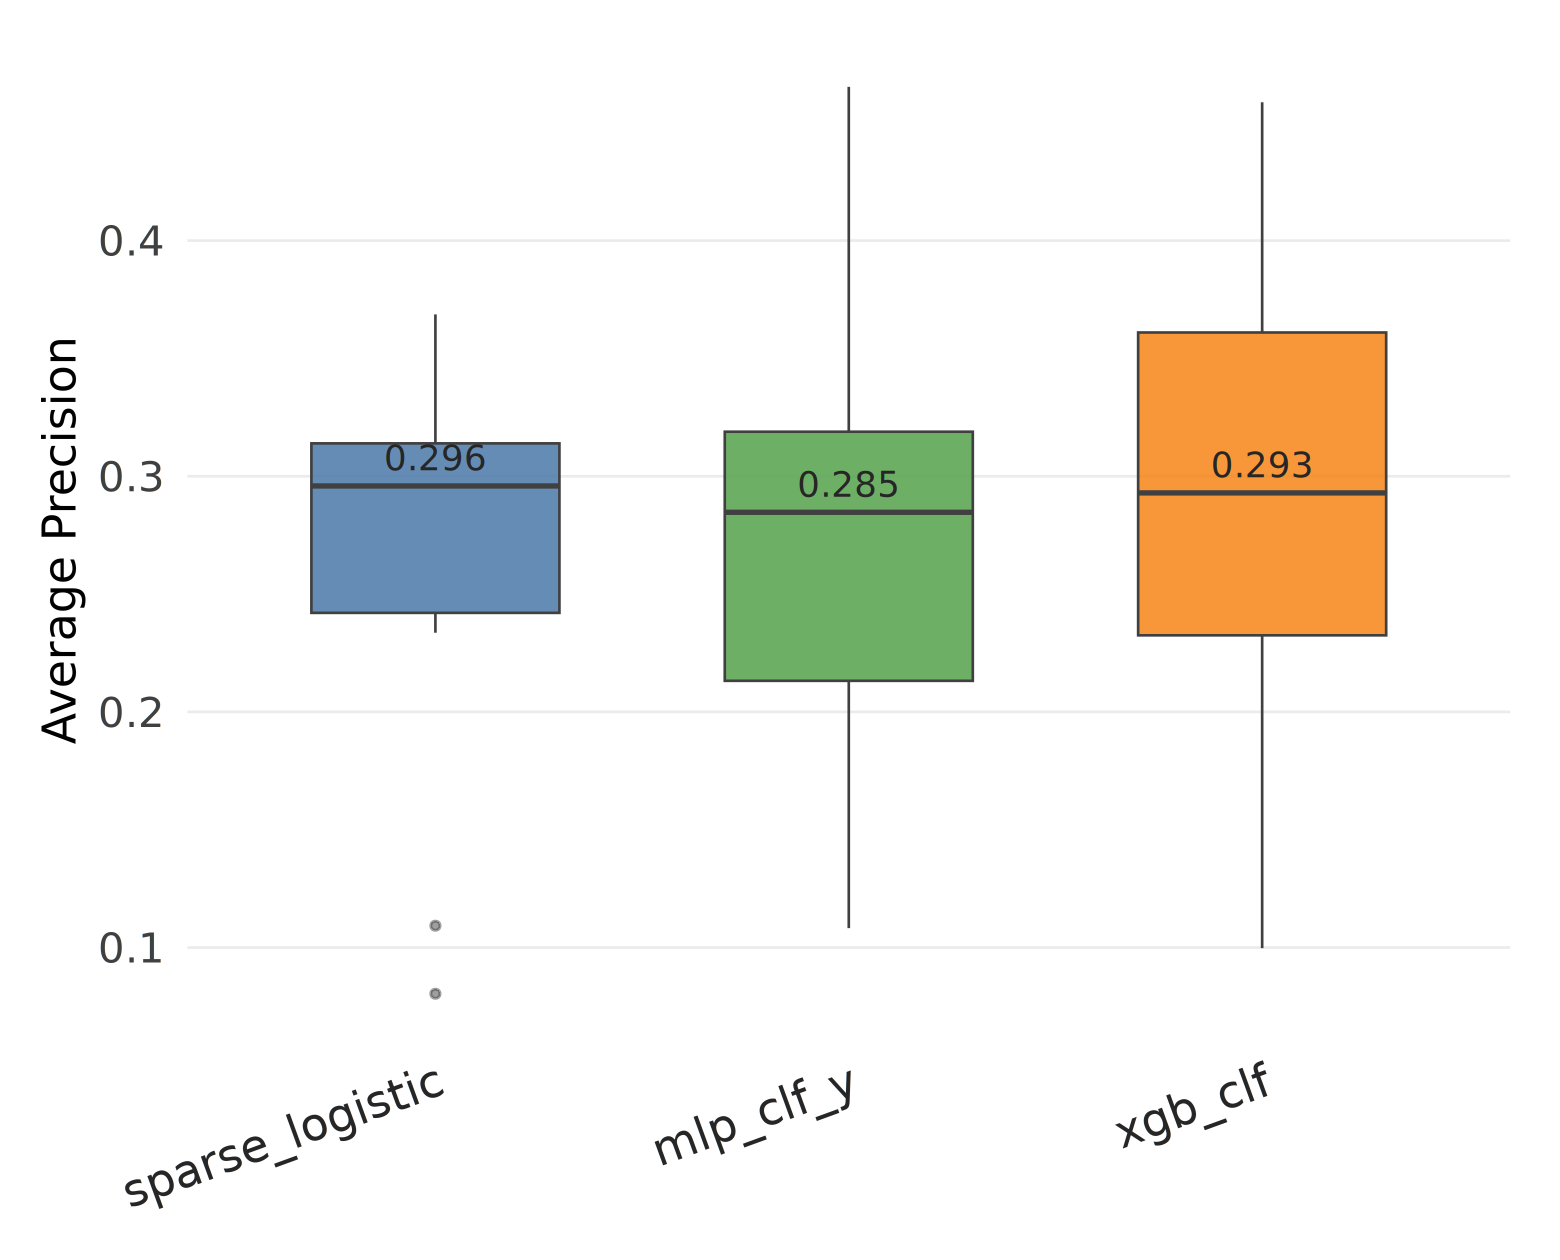
\includegraphics[width=\linewidth]{figures/fig_ap_y_ap_baseline_ibd.png}
    \caption{IBD}
  \end{subfigure}\hfill
  \begin{subfigure}[t]{0.32\textwidth}
    \centering
    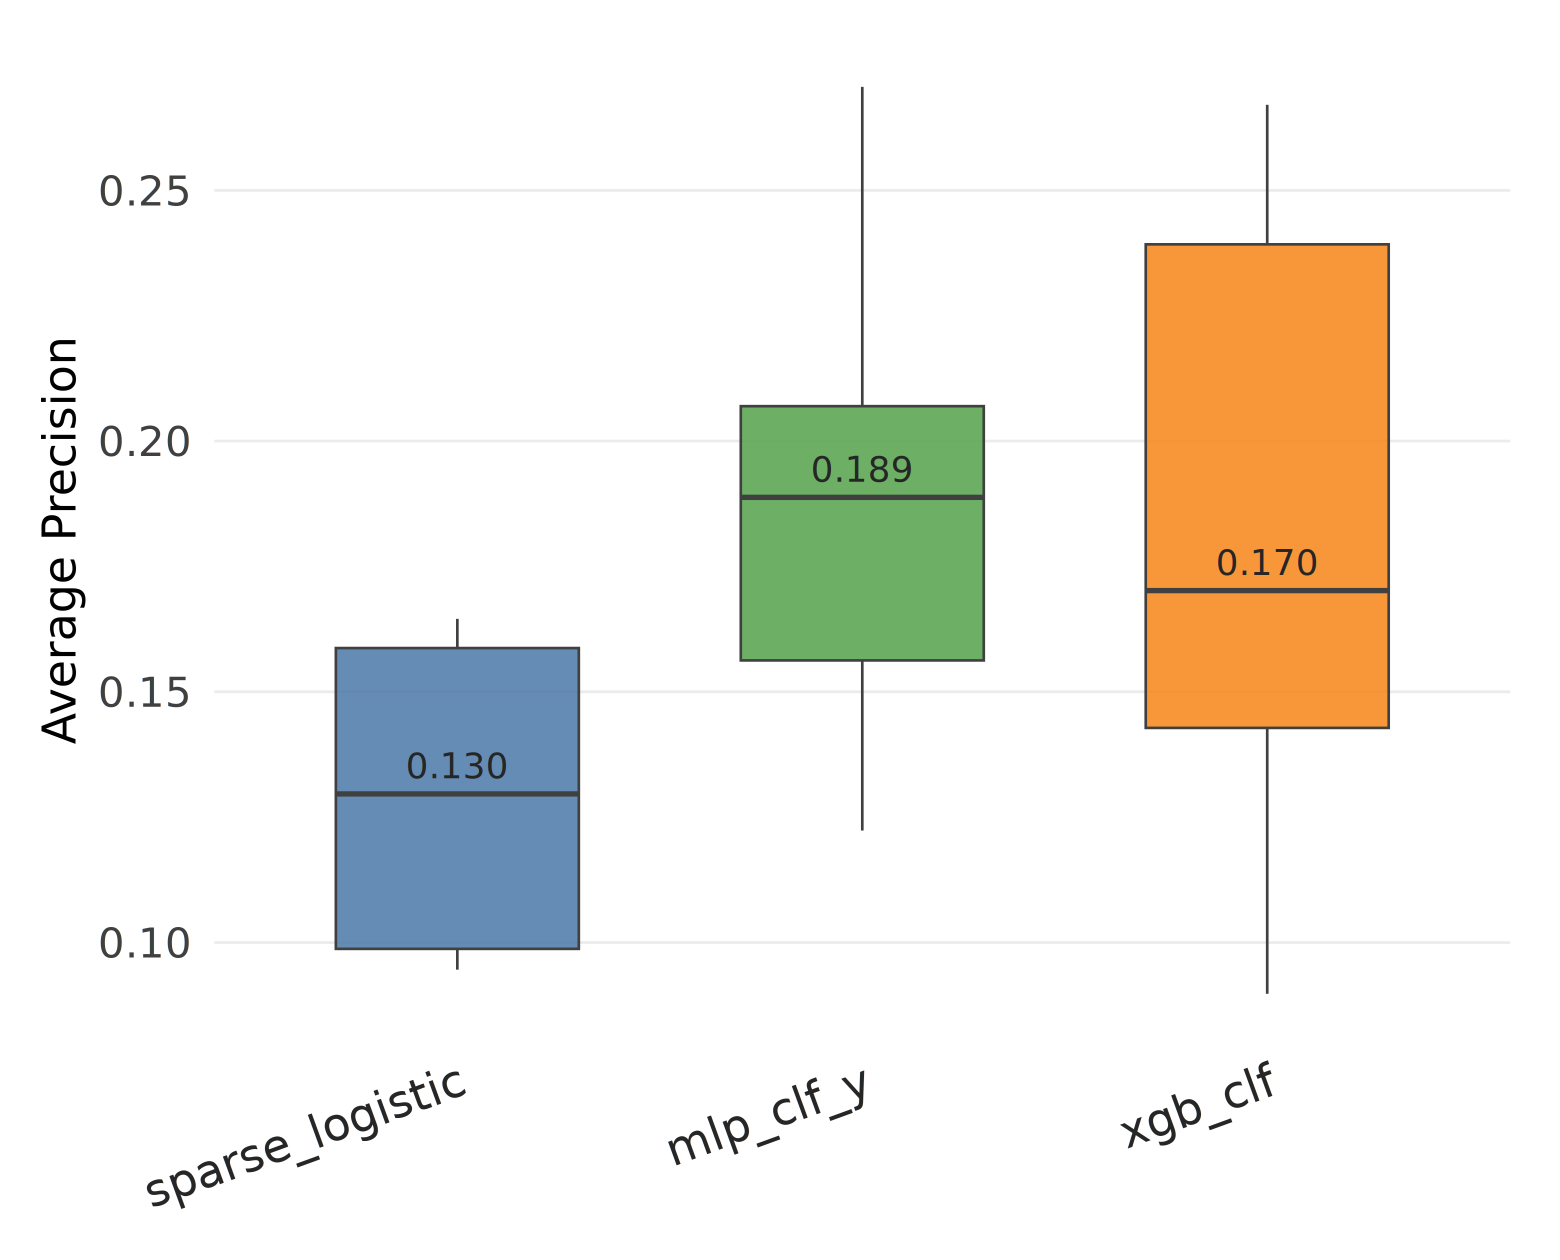
\includegraphics[width=\linewidth]{figures/fig_ap_y_ap_baseline_gvhd.png}
    \caption{GvHD}
  \end{subfigure}
  \caption{Test AP on CRISPR linkage, baseline models}
  \label{fig:ap-yapb}
\end{figure}

\begin{figure}[H]
  \centering
  \begin{subfigure}[t]{0.32\textwidth}
    \centering
    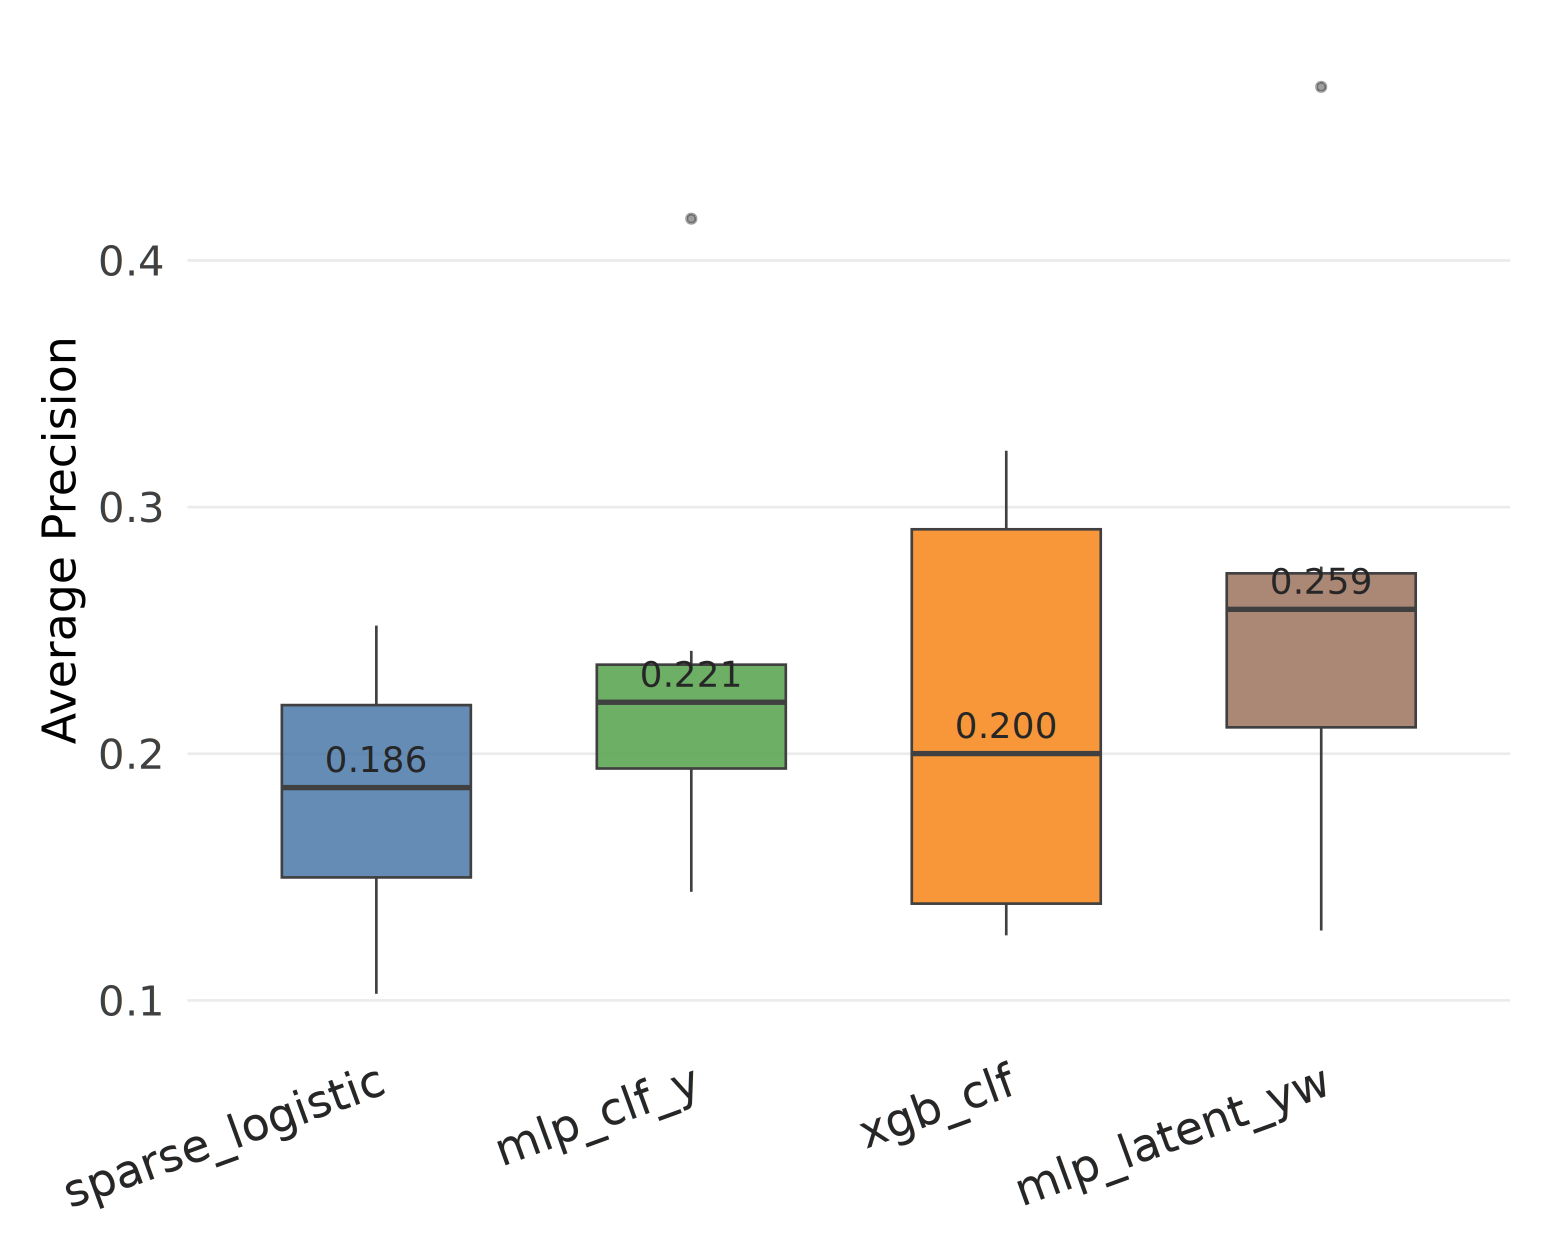
\includegraphics[width=\linewidth]{figures/fig_ap_y_ap_all_crc.png}
    \caption{CRC}
  \end{subfigure}\hfill
  \begin{subfigure}[t]{0.32\textwidth}
    \centering
    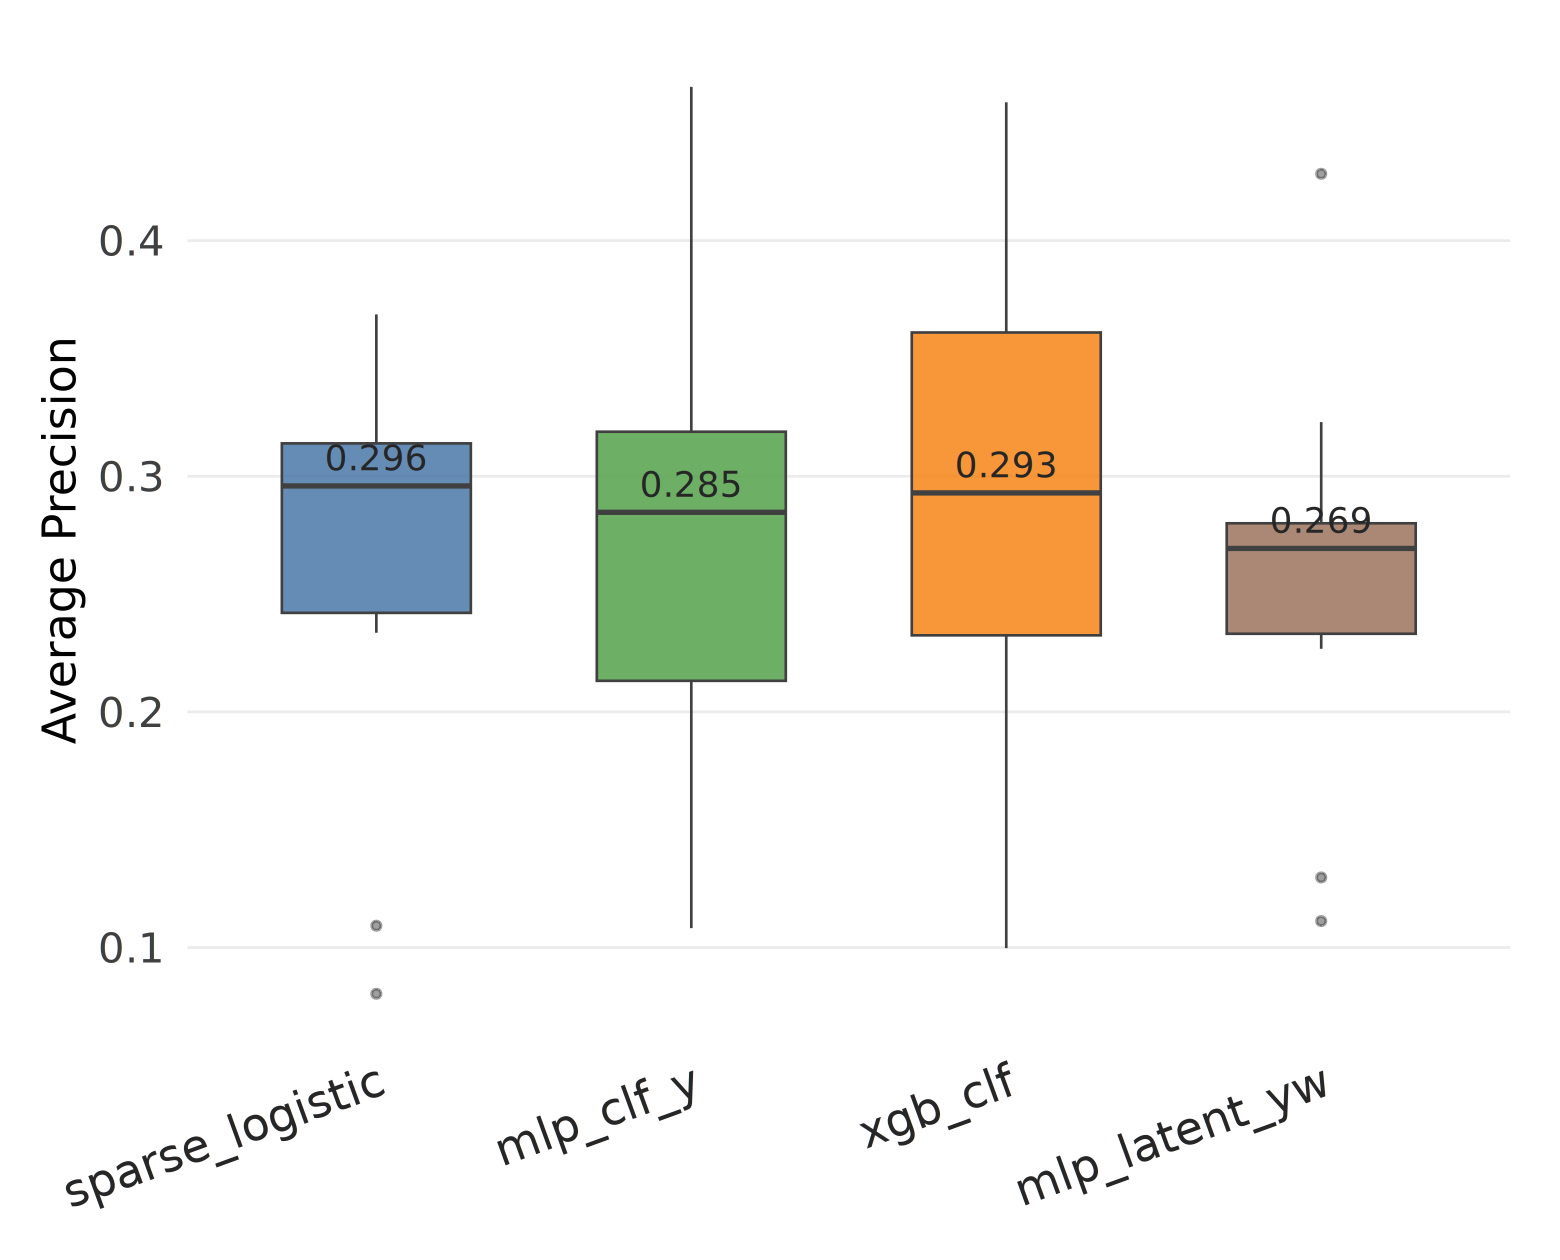
\includegraphics[width=\linewidth]{figures/fig_ap_y_ap_all_ibd.png}
    \caption{IBD}
  \end{subfigure}\hfill
  \begin{subfigure}[t]{0.32\textwidth}
    \centering
    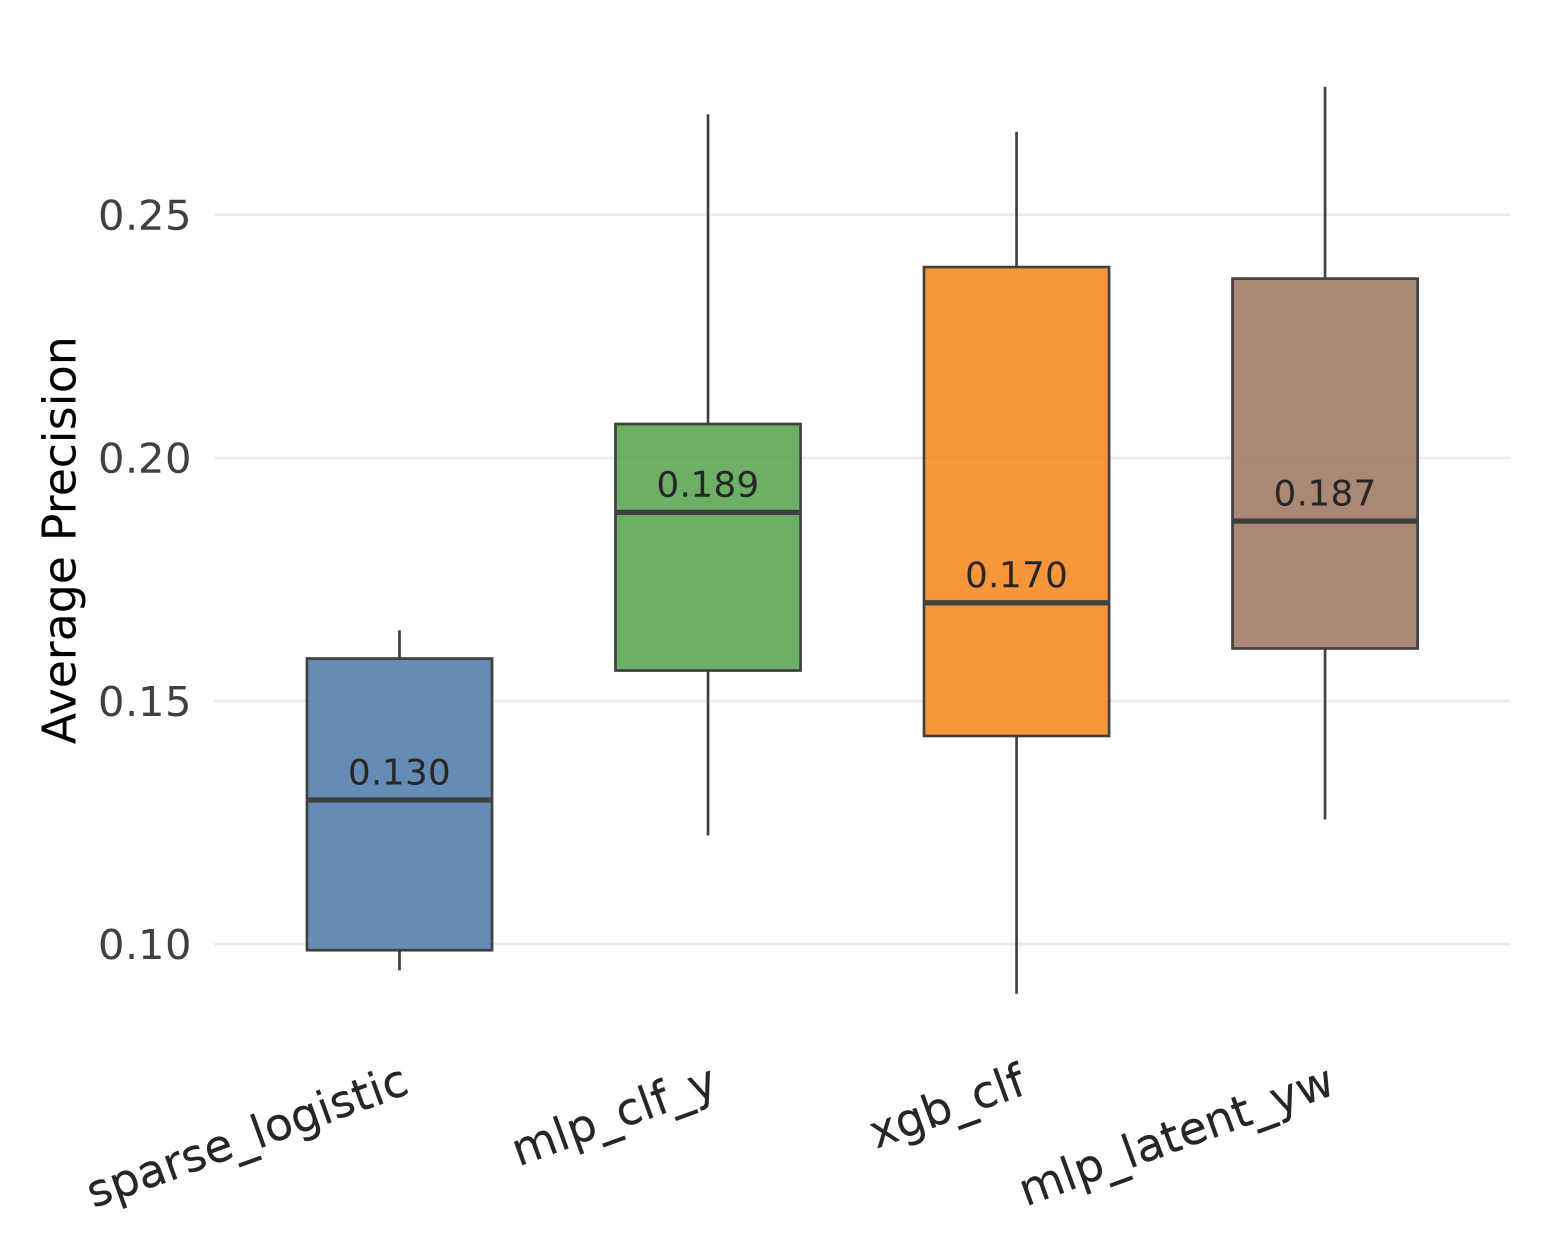
\includegraphics[width=\linewidth]{figures/fig_ap_y_ap_all_gvhd.png}
    \caption{GvHD}
  \end{subfigure}
  \caption{Test AP on CRISPR linkage, all models}
  \label{fig:ap-yapa}
\end{figure}

\begin{figure}[H]
  \centering
  \begin{subfigure}[t]{0.32\textwidth}
    \centering
    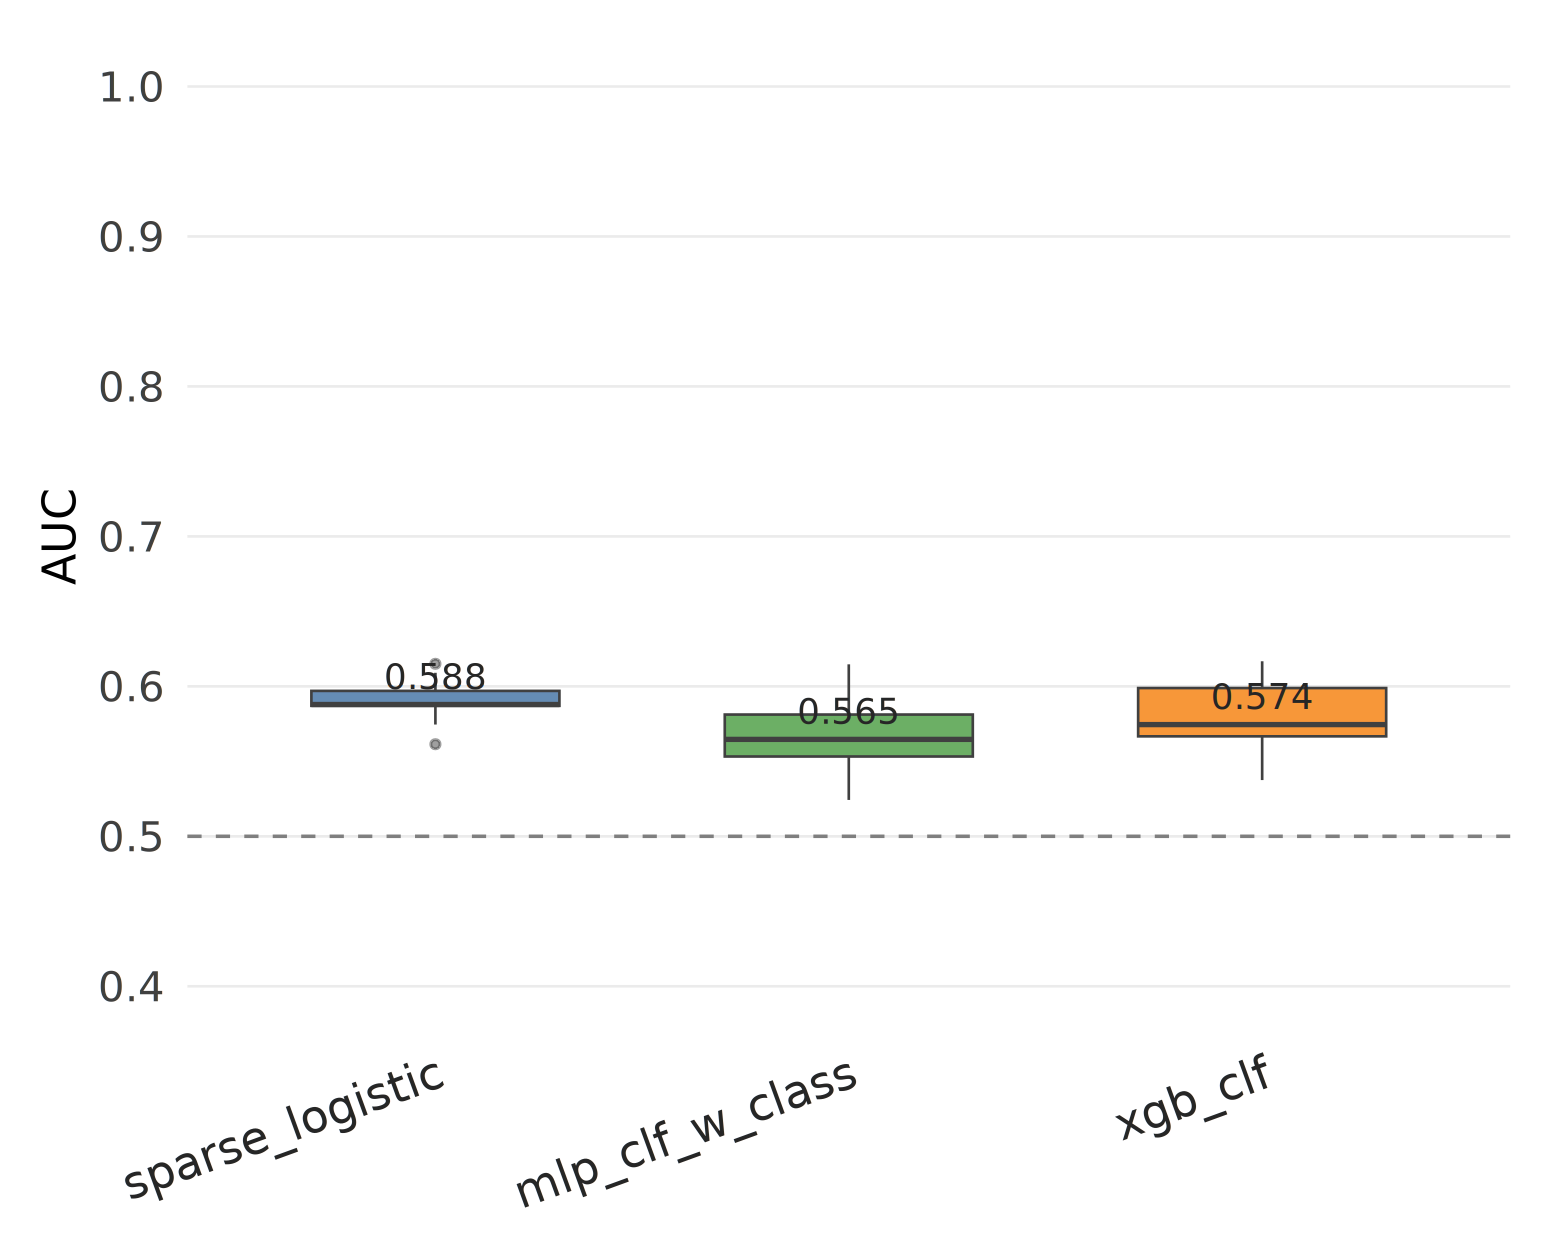
\includegraphics[width=\linewidth]{figures/fig_ap_w_class_auc_baseline_crc.png}
    \caption{CRC}
  \end{subfigure}\hfill
  \begin{subfigure}[t]{0.32\textwidth}
    \centering
    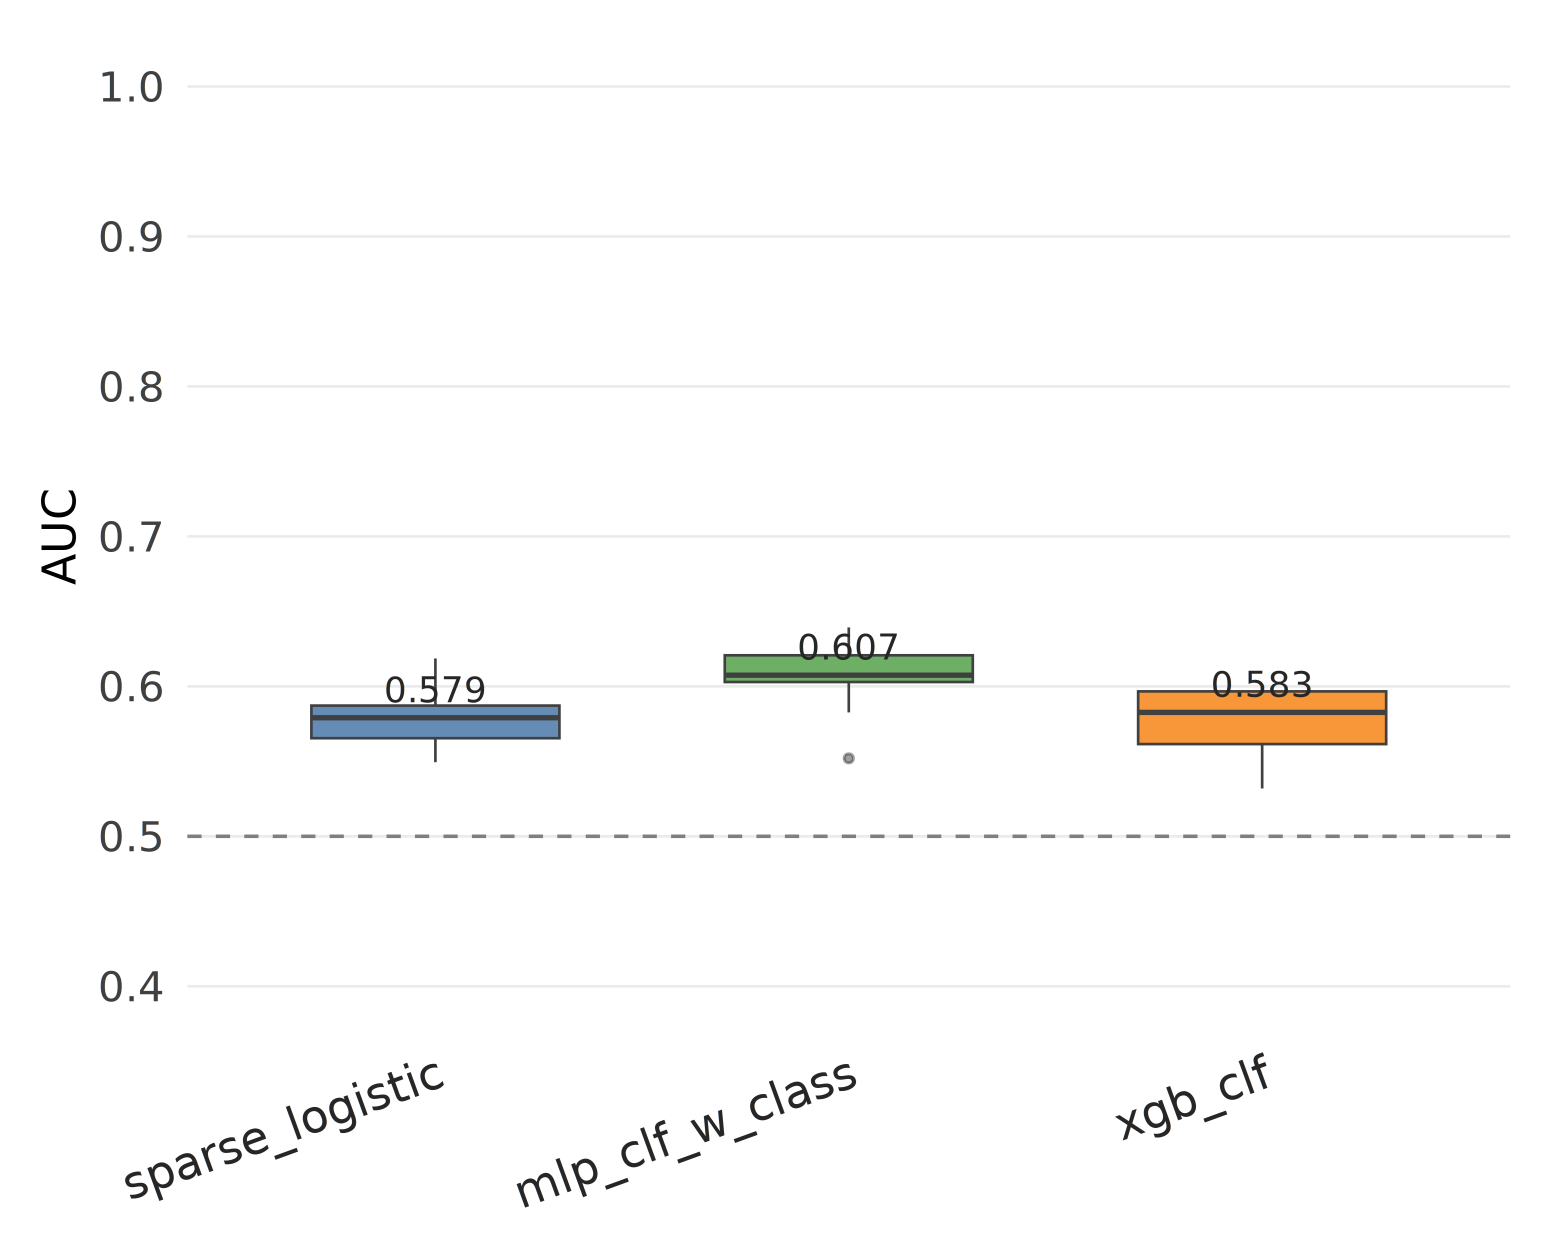
\includegraphics[width=\linewidth]{figures/fig_ap_w_class_auc_baseline_ibd.png}
    \caption{IBD}
  \end{subfigure}\hfill
  \begin{subfigure}[t]{0.32\textwidth}
    \centering
    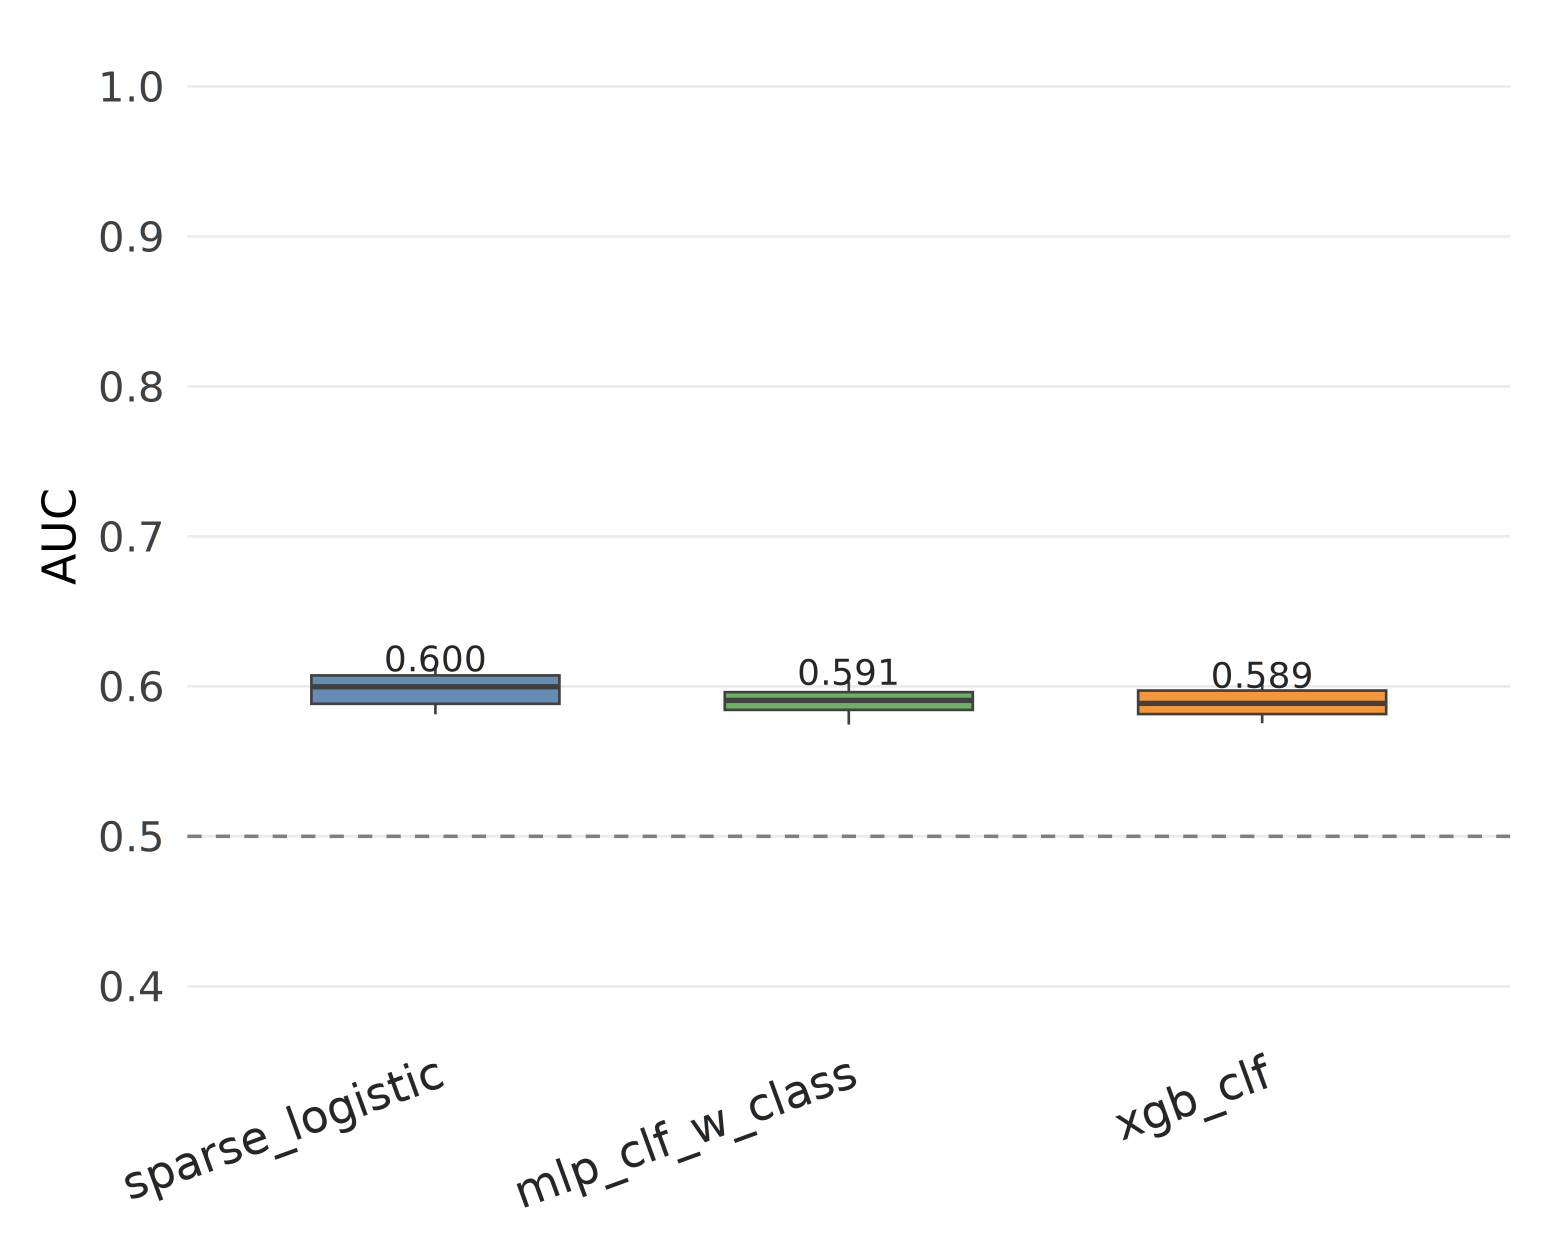
\includegraphics[width=\linewidth]{figures/fig_ap_w_class_auc_baseline_gvhd.png}
    \caption{GvHD}
  \end{subfigure}
  \caption{Test AUC on the binarised selection probability, baseline models}
  \label{fig:ap-wcaucb}
\end{figure}

\begin{figure}[H]
  \centering
  \begin{subfigure}[t]{0.32\textwidth}
    \centering
    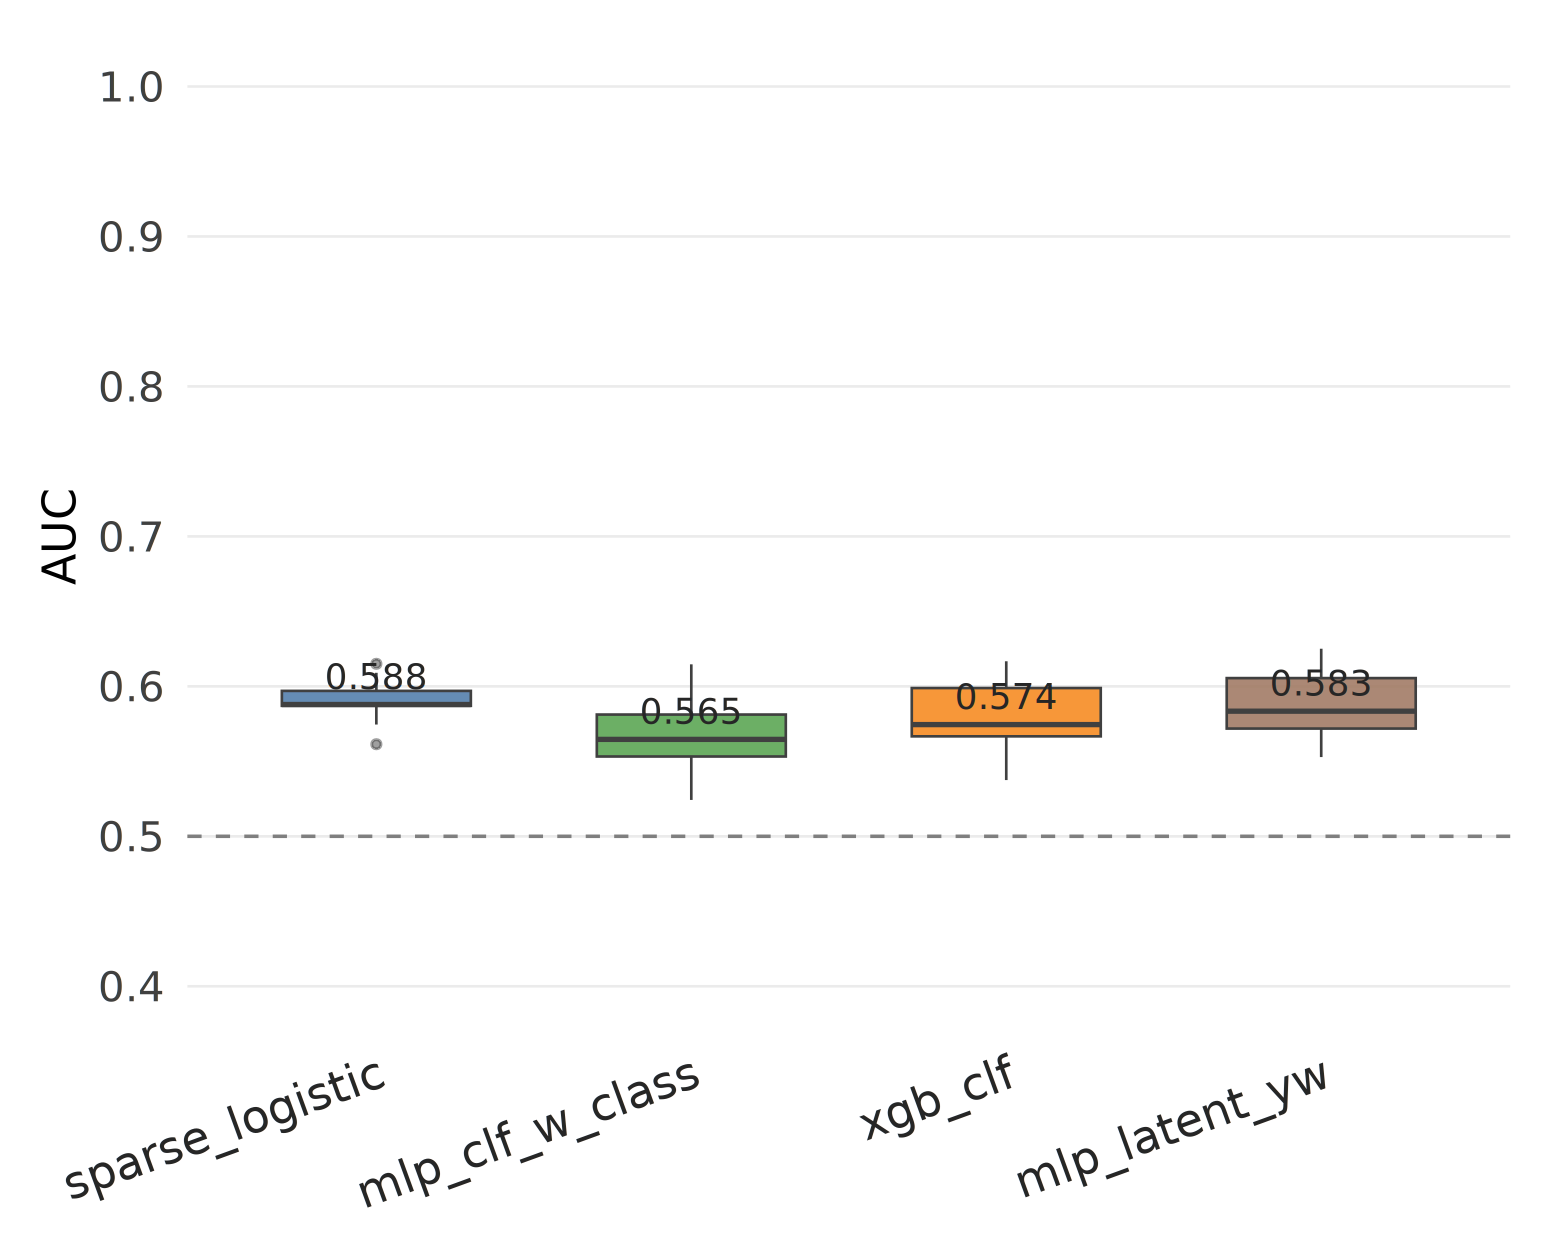
\includegraphics[width=\linewidth]{figures/fig_ap_w_class_auc_all_crc.png}
    \caption{CRC}
  \end{subfigure}\hfill
  \begin{subfigure}[t]{0.32\textwidth}
    \centering
    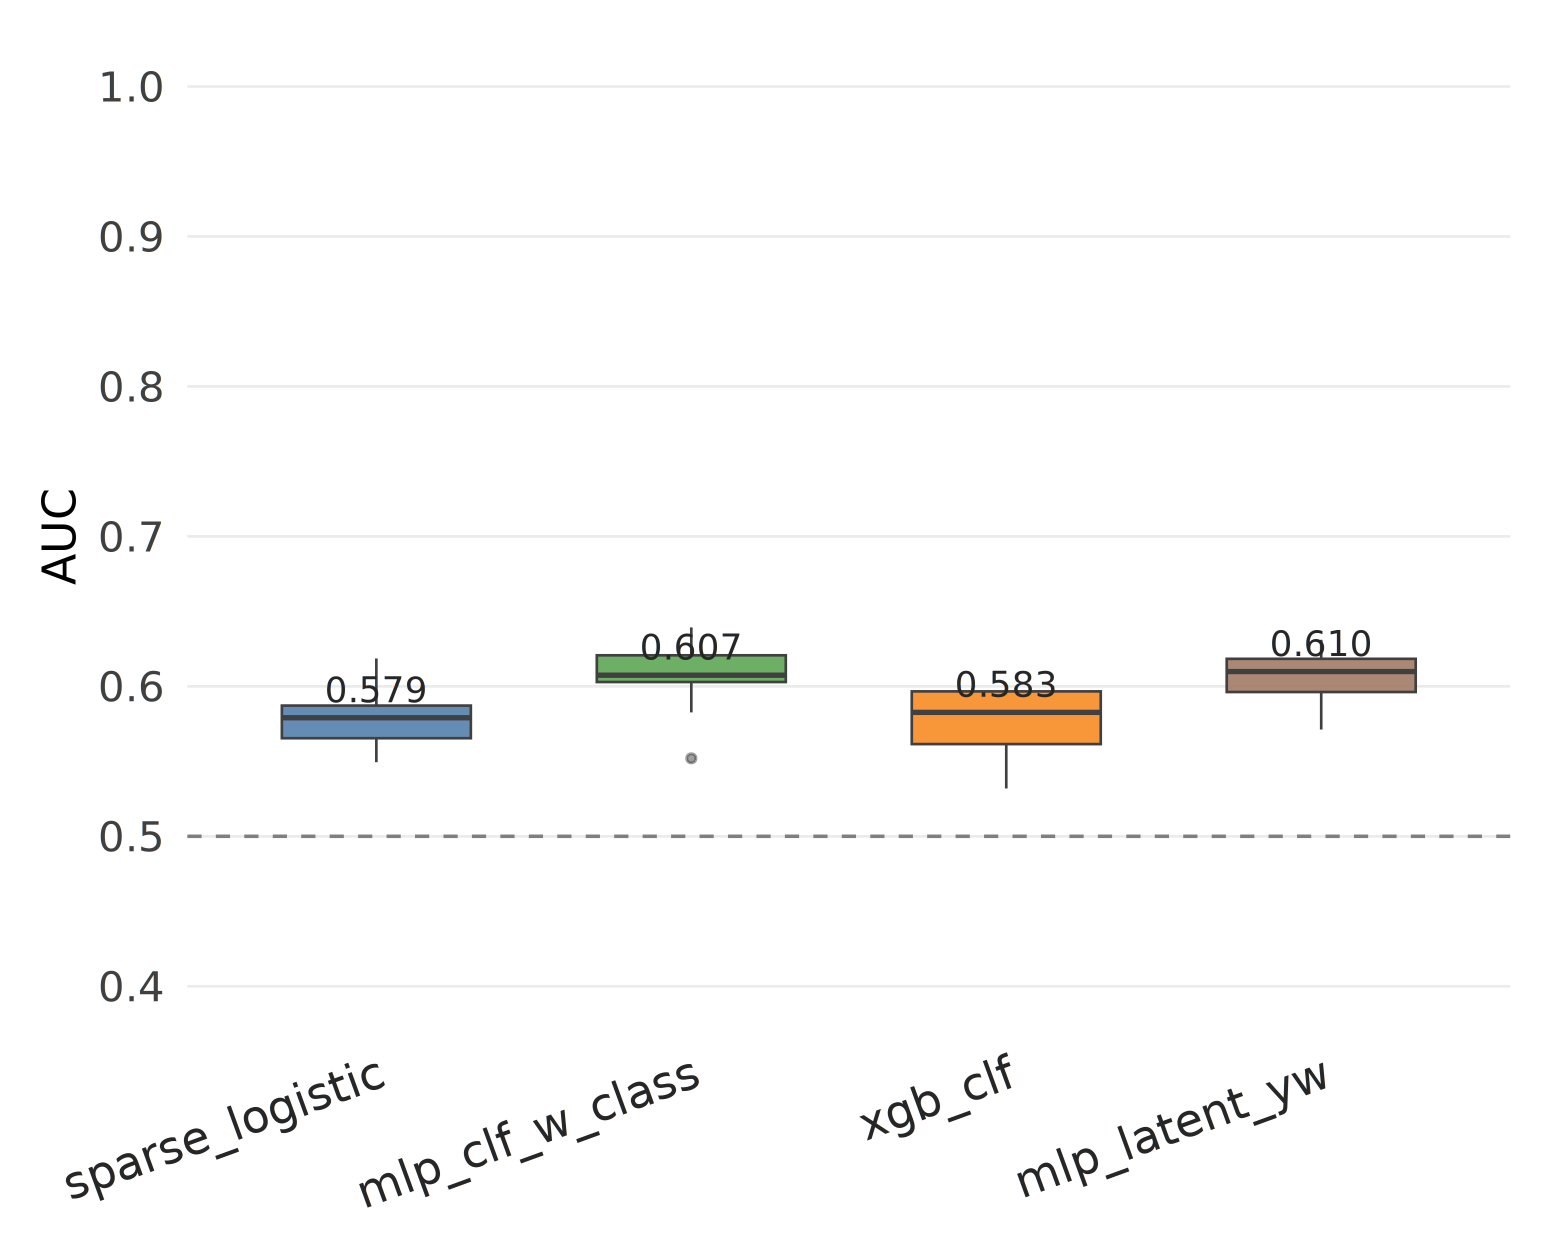
\includegraphics[width=\linewidth]{figures/fig_ap_w_class_auc_all_ibd.png}
    \caption{IBD}
  \end{subfigure}\hfill
  \begin{subfigure}[t]{0.32\textwidth}
    \centering
    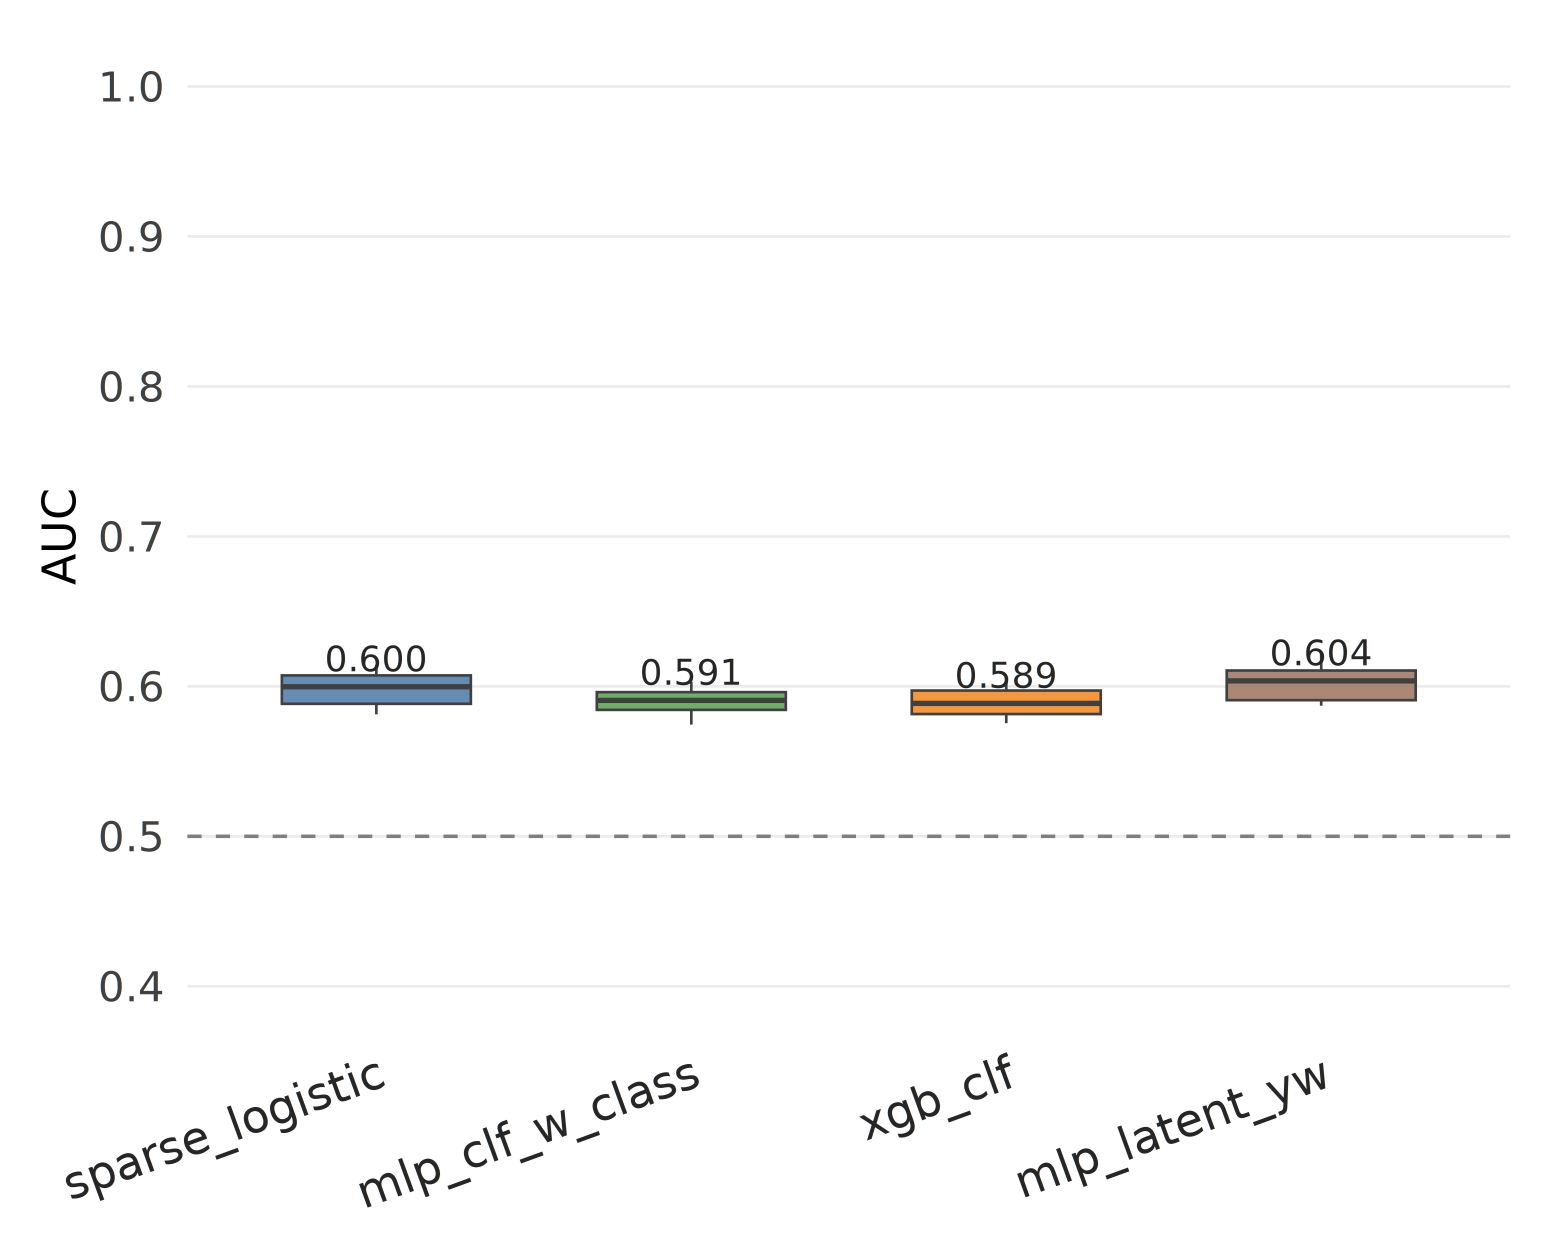
\includegraphics[width=\linewidth]{figures/fig_ap_w_class_auc_all_gvhd.png}
    \caption{GvHD}
  \end{subfigure}
  \caption{Test AUC on the binarised selection probability, all models}
  \label{fig:ap-wcauca}
\end{figure}

\begin{figure}[H]
  \centering
  \begin{subfigure}[t]{0.32\textwidth}
    \centering
    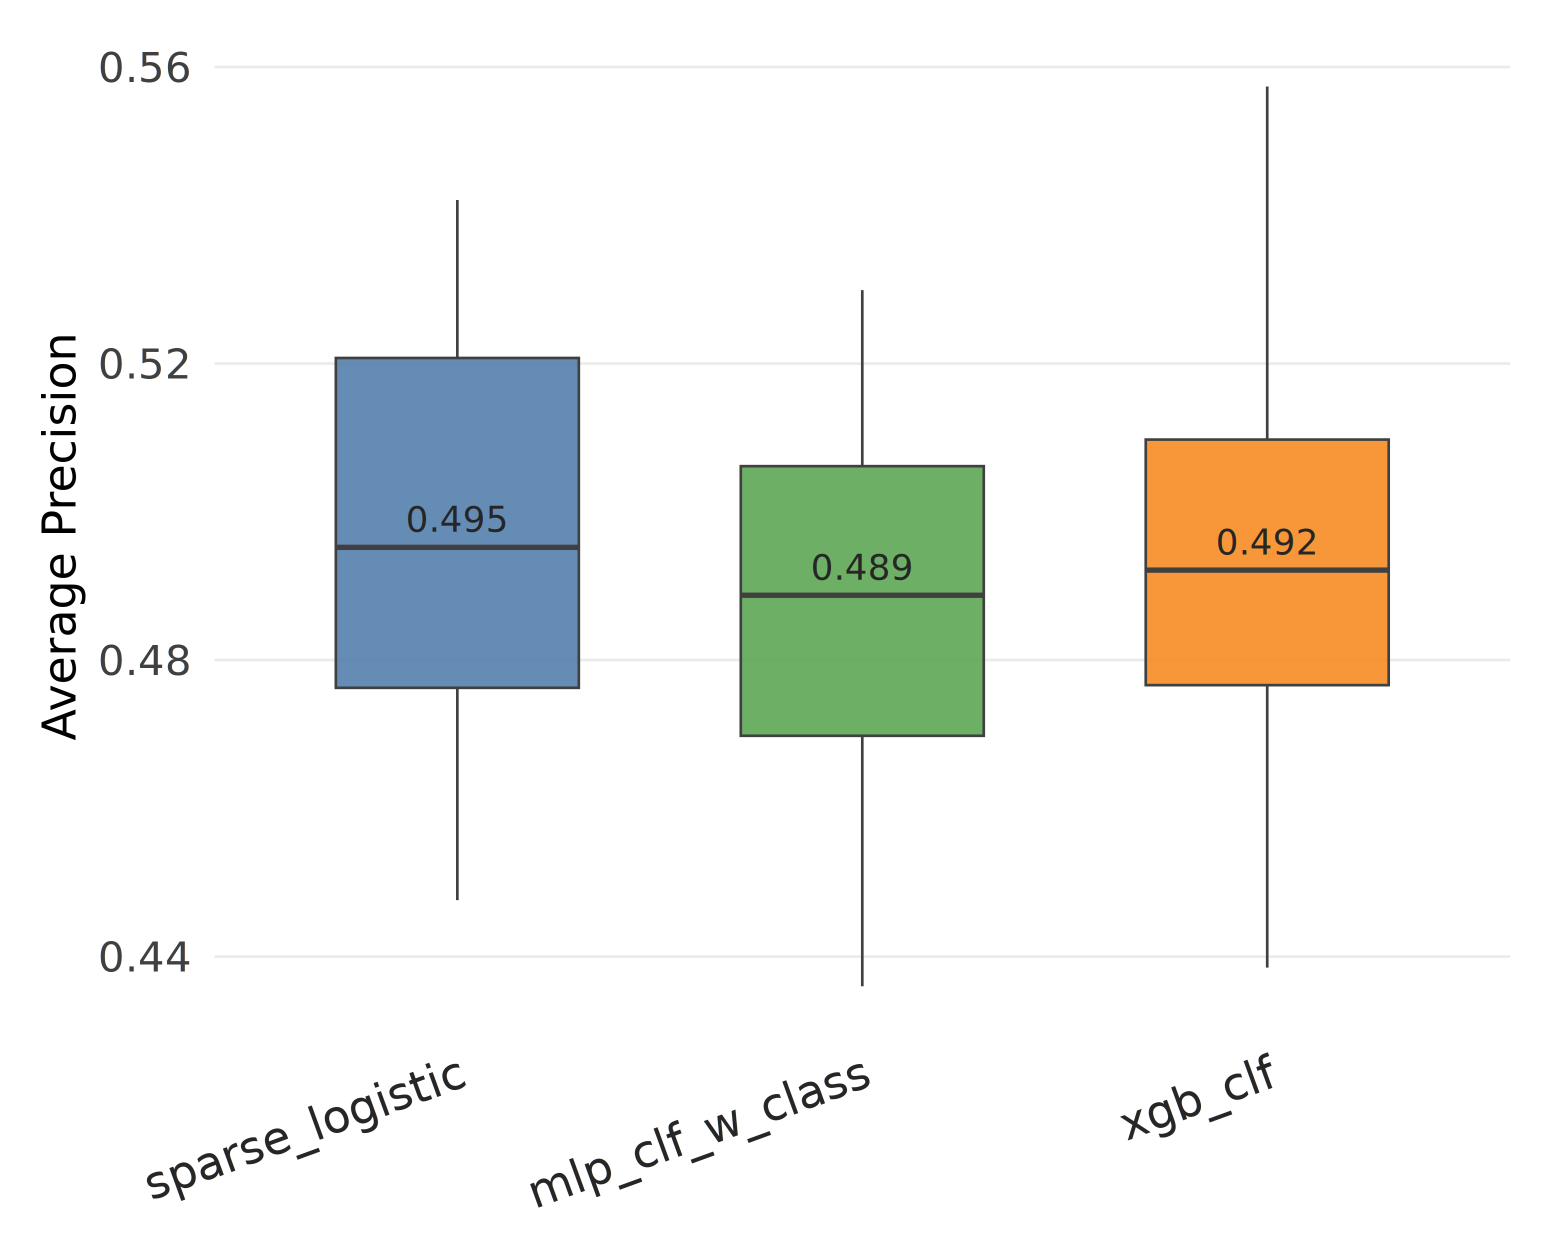
\includegraphics[width=\linewidth]{figures/fig_ap_w_class_ap_baseline_crc.png}
    \caption{CRC}
  \end{subfigure}\hfill
  \begin{subfigure}[t]{0.32\textwidth}
    \centering
    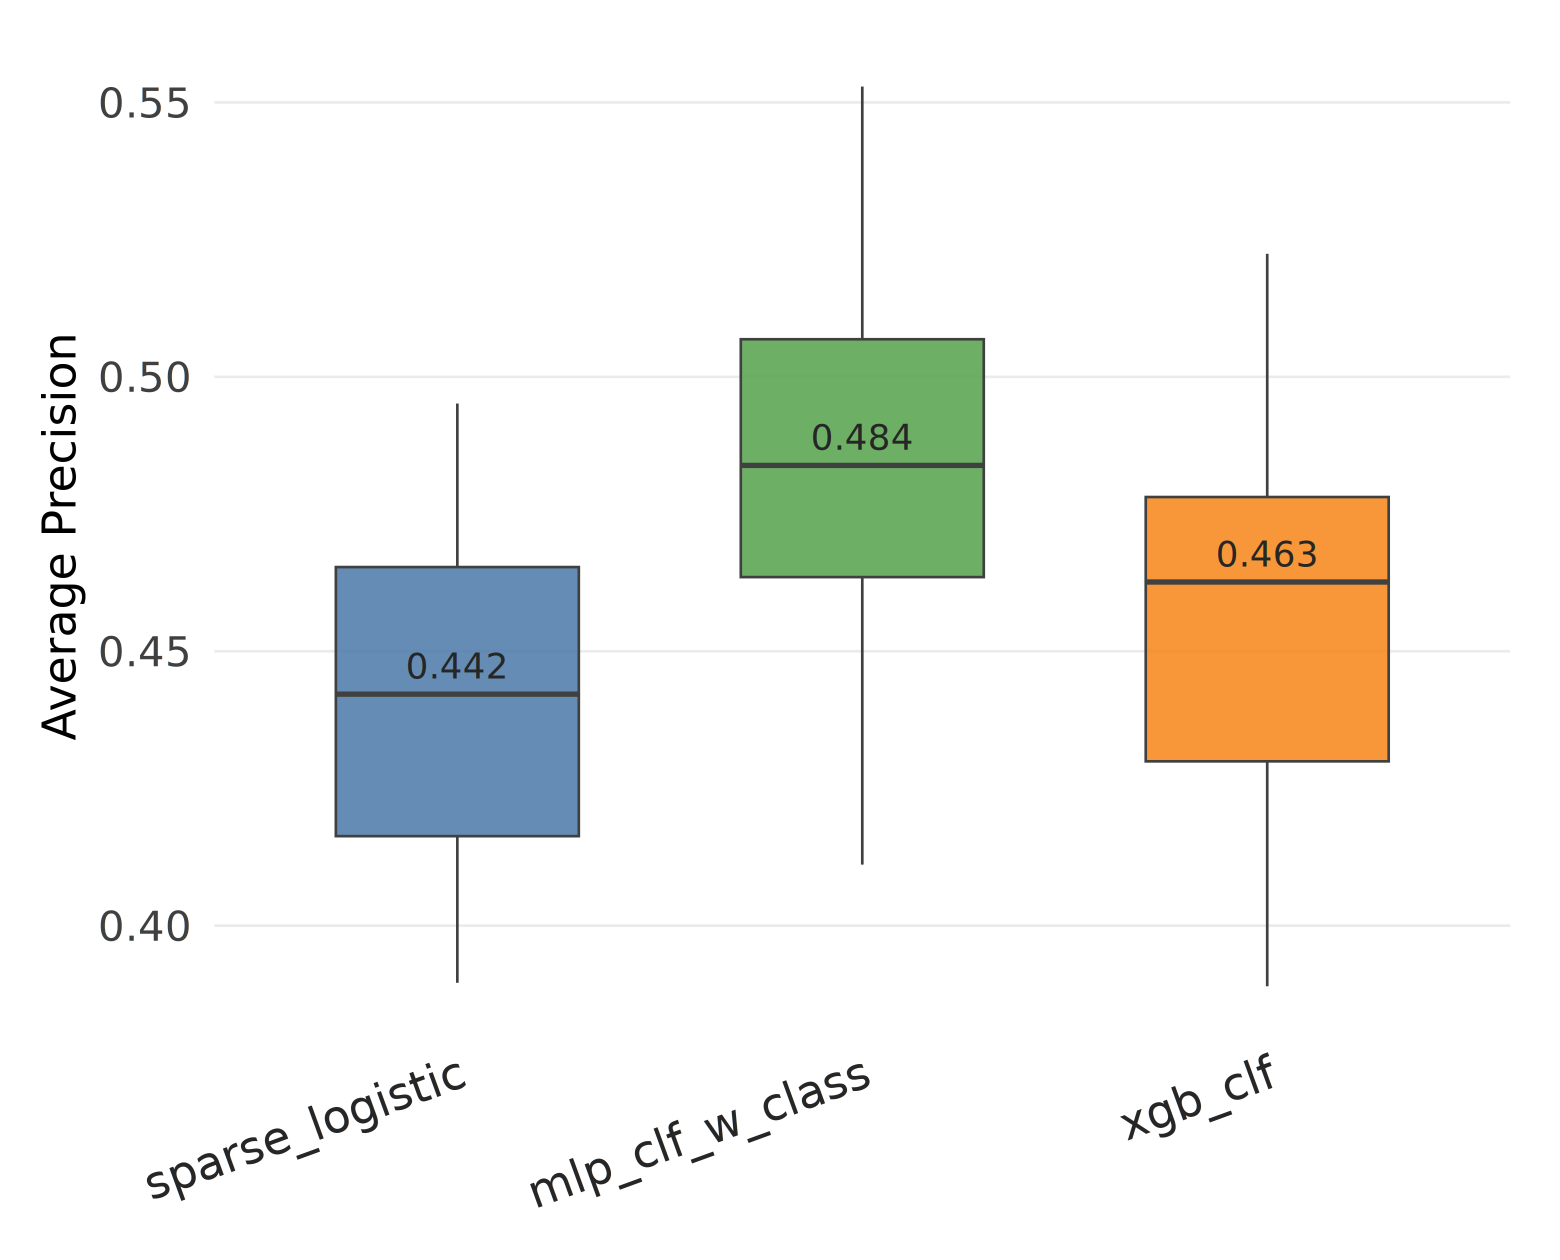
\includegraphics[width=\linewidth]{figures/fig_ap_w_class_ap_baseline_ibd.png}
    \caption{IBD}
  \end{subfigure}\hfill
  \begin{subfigure}[t]{0.32\textwidth}
    \centering
    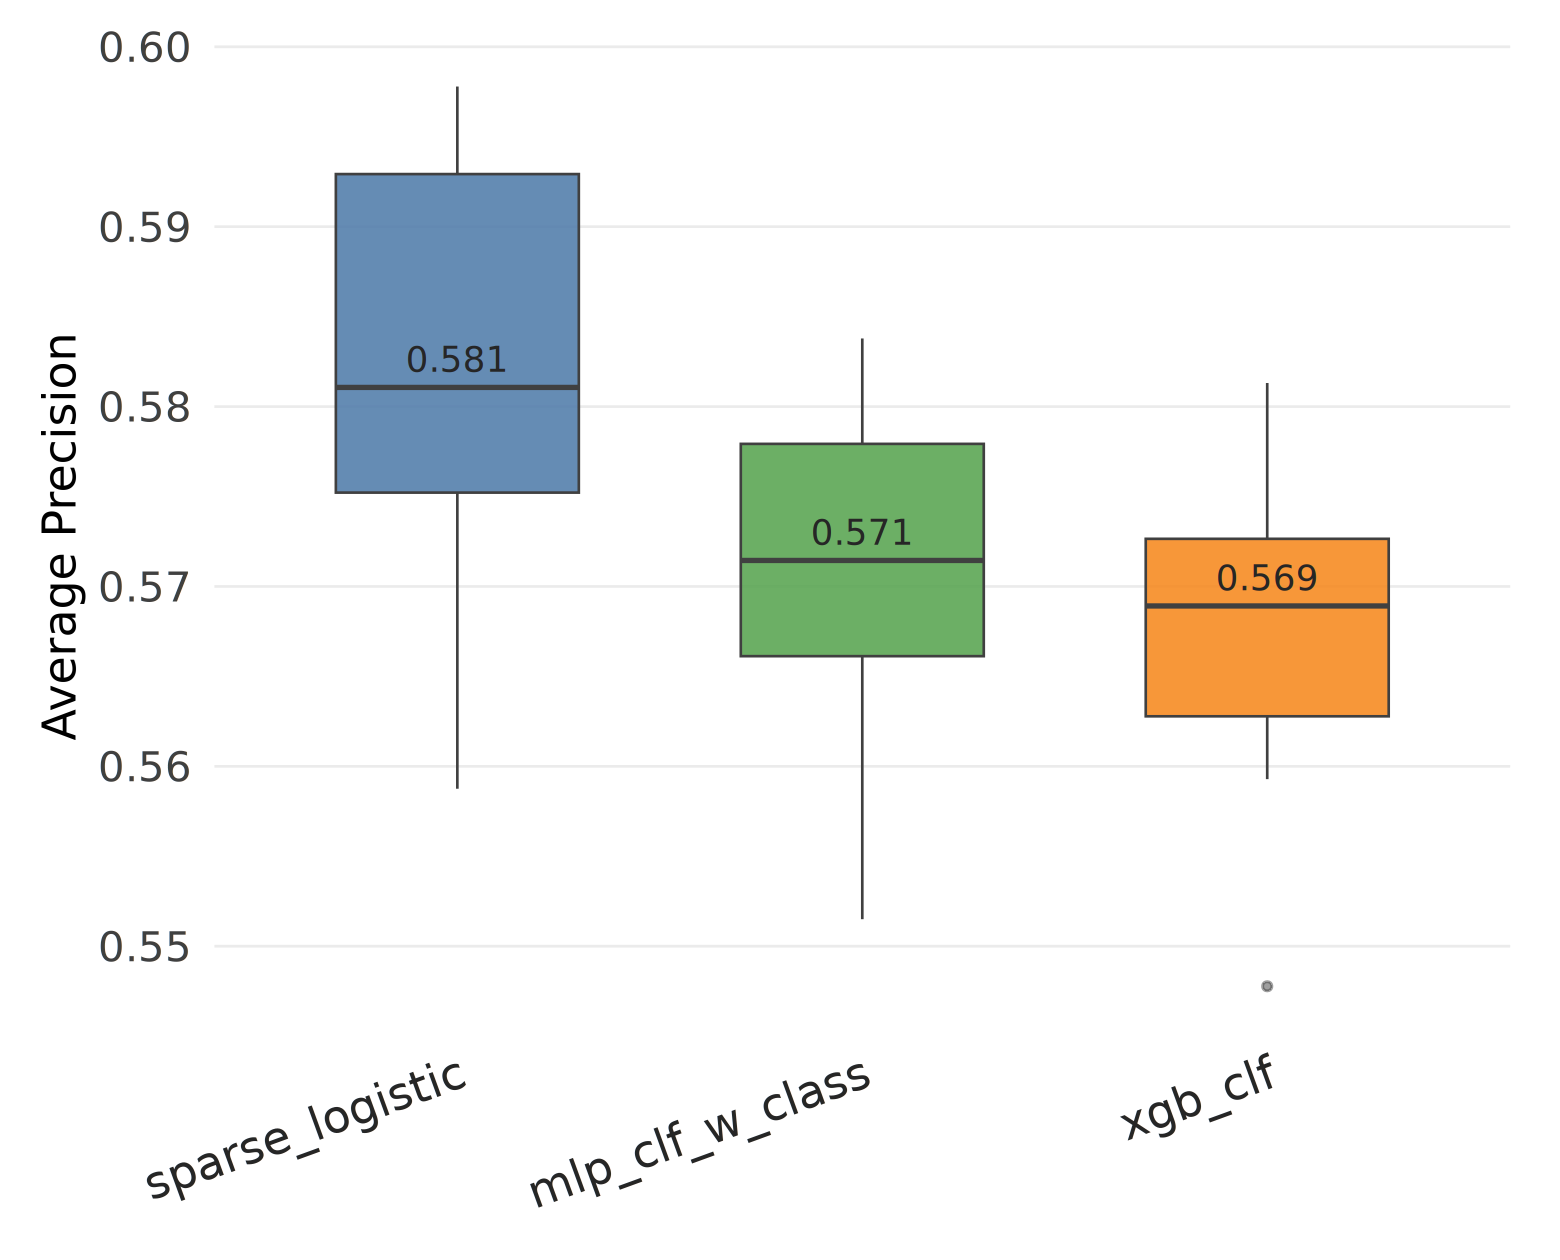
\includegraphics[width=\linewidth]{figures/fig_ap_w_class_ap_baseline_gvhd.png}
    \caption{GvHD}
  \end{subfigure}
  \caption{Test AP on the binarised selection probability, baseline models}
  \label{fig:ap-wcapb}
\end{figure}

\begin{figure}[H]
  \centering
  \begin{subfigure}[t]{0.32\textwidth}
    \centering
    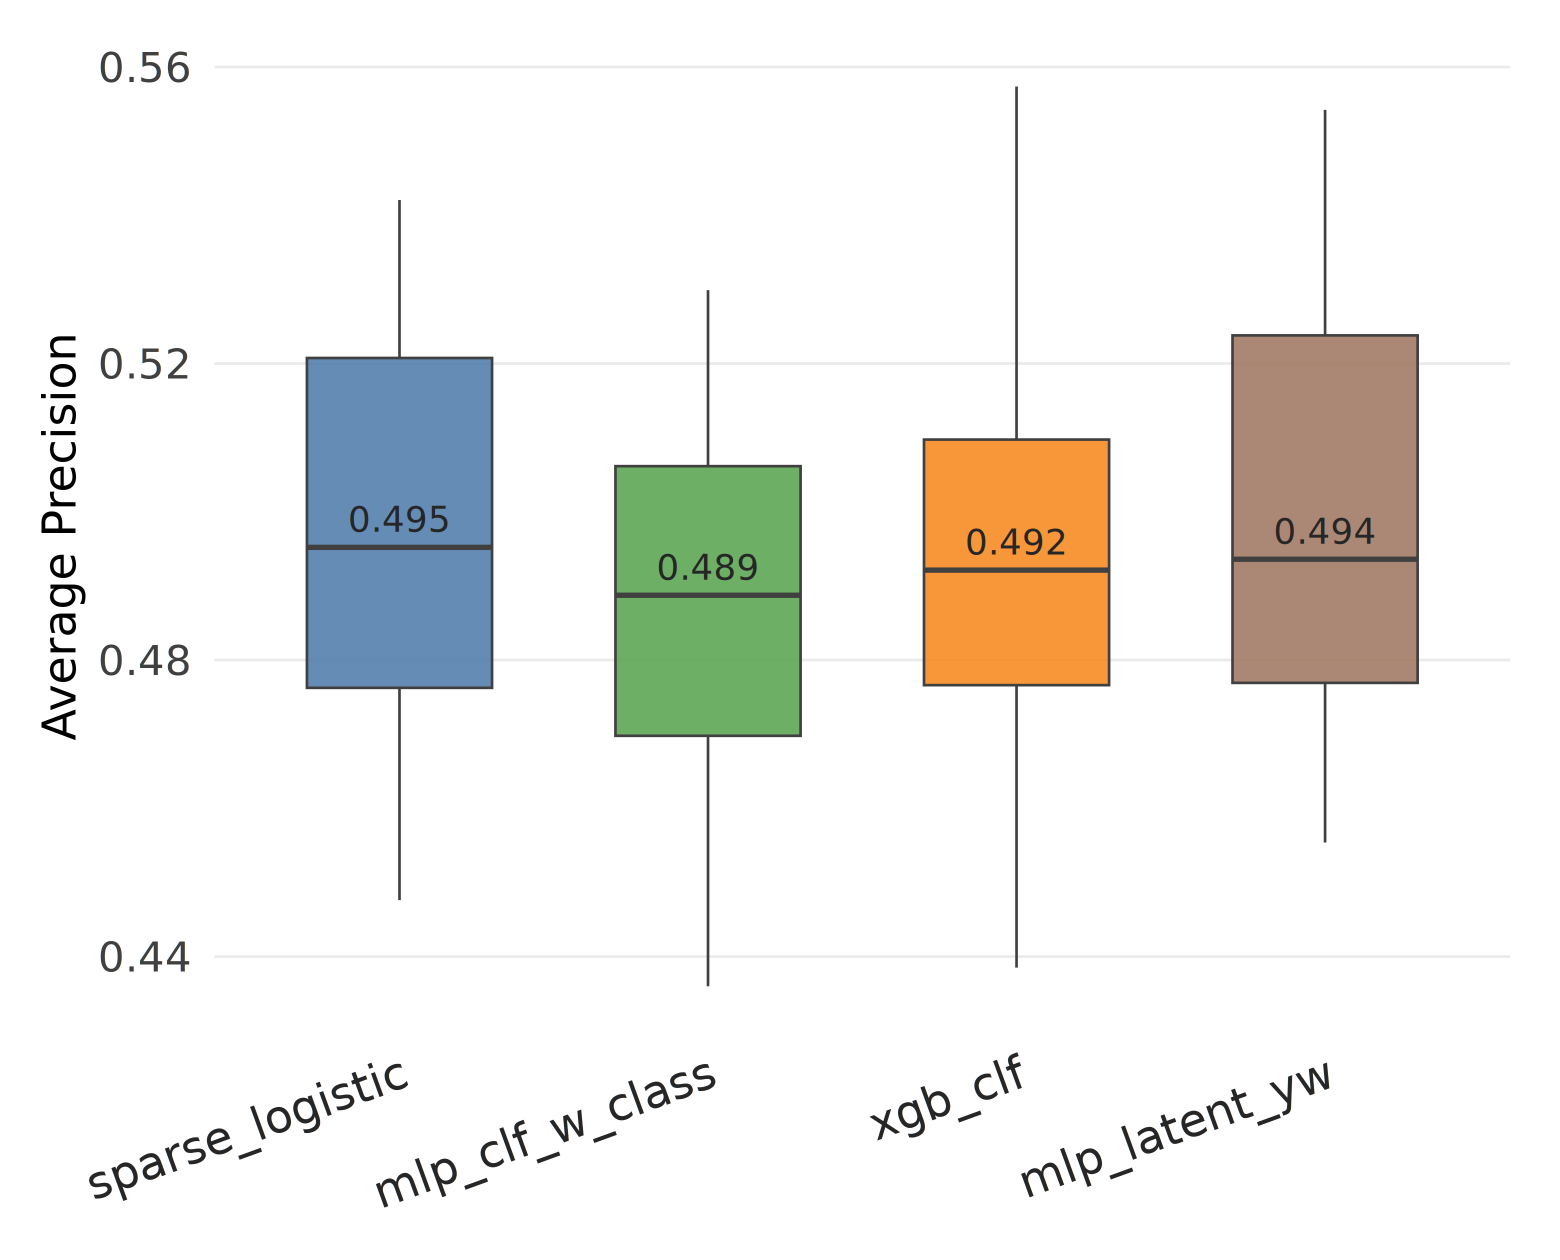
\includegraphics[width=\linewidth]{figures/fig_ap_w_class_ap_all_crc.png}
    \caption{CRC}
  \end{subfigure}\hfill
  \begin{subfigure}[t]{0.32\textwidth}
    \centering
    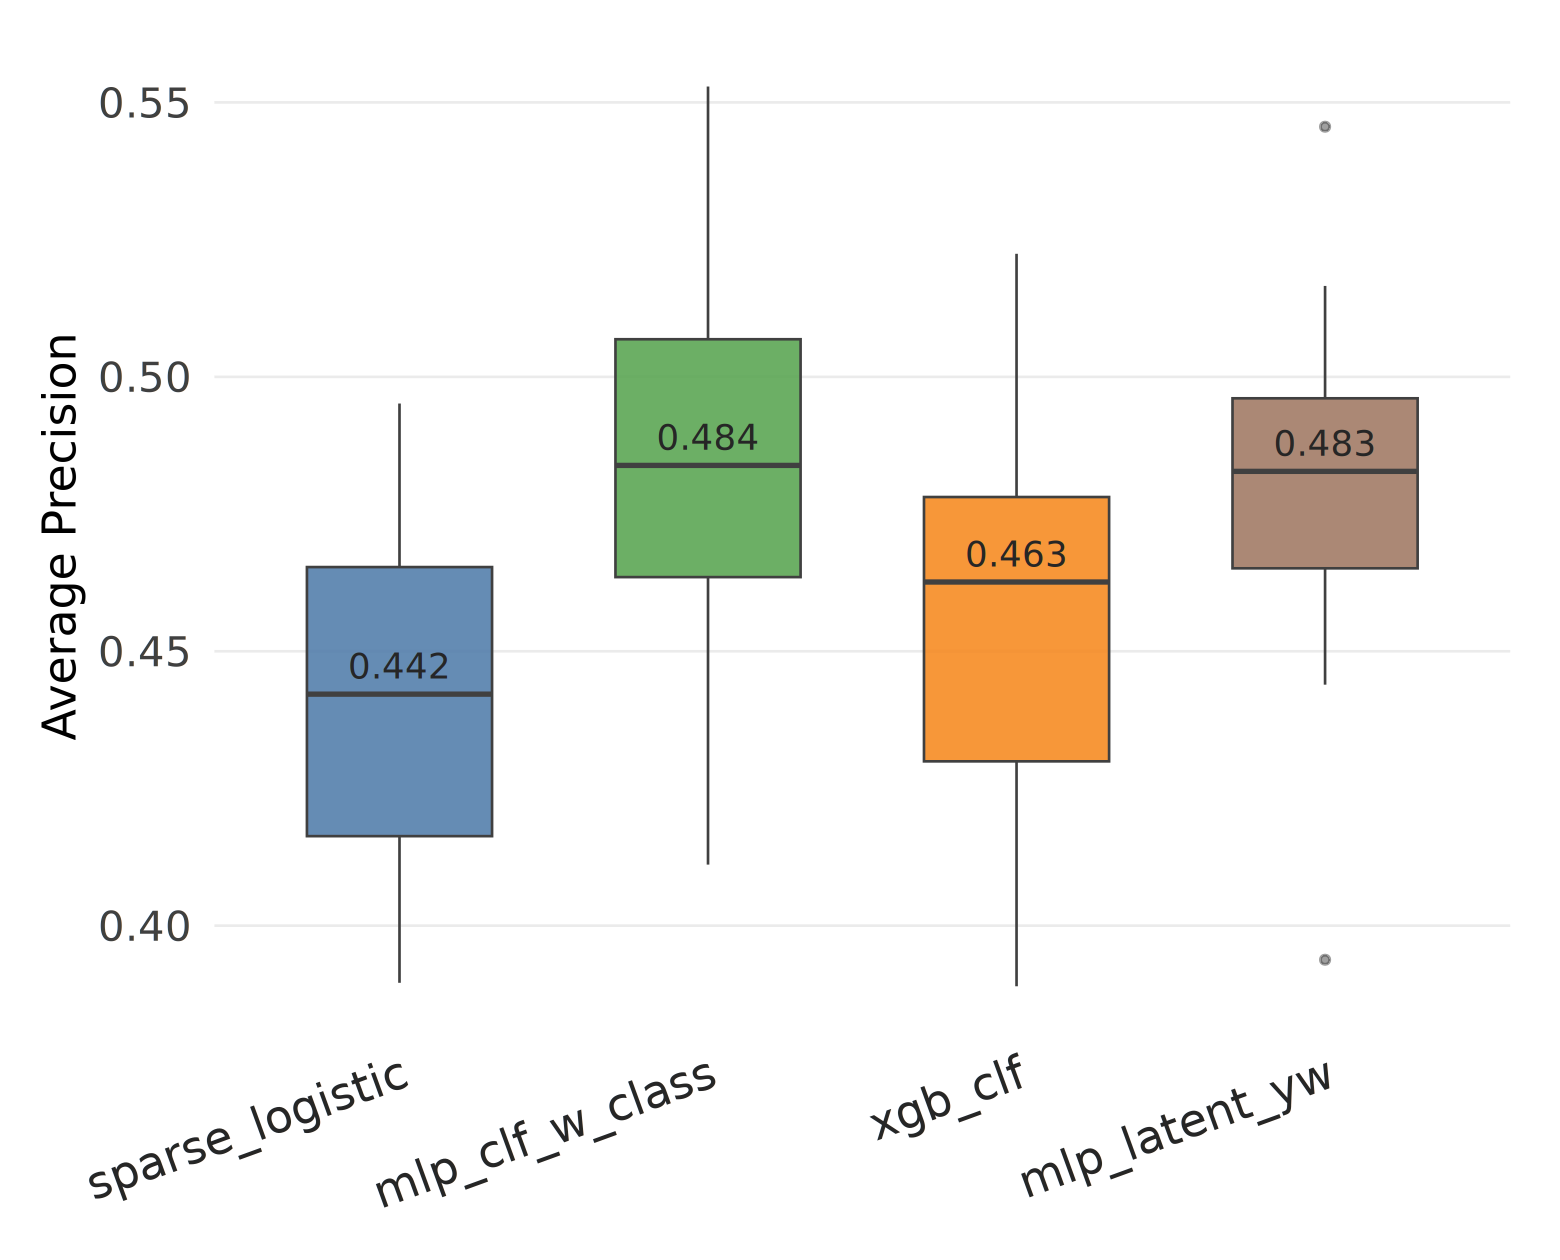
\includegraphics[width=\linewidth]{figures/fig_ap_w_class_ap_all_ibd.png}
    \caption{IBD}
  \end{subfigure}\hfill
  \begin{subfigure}[t]{0.32\textwidth}
    \centering
    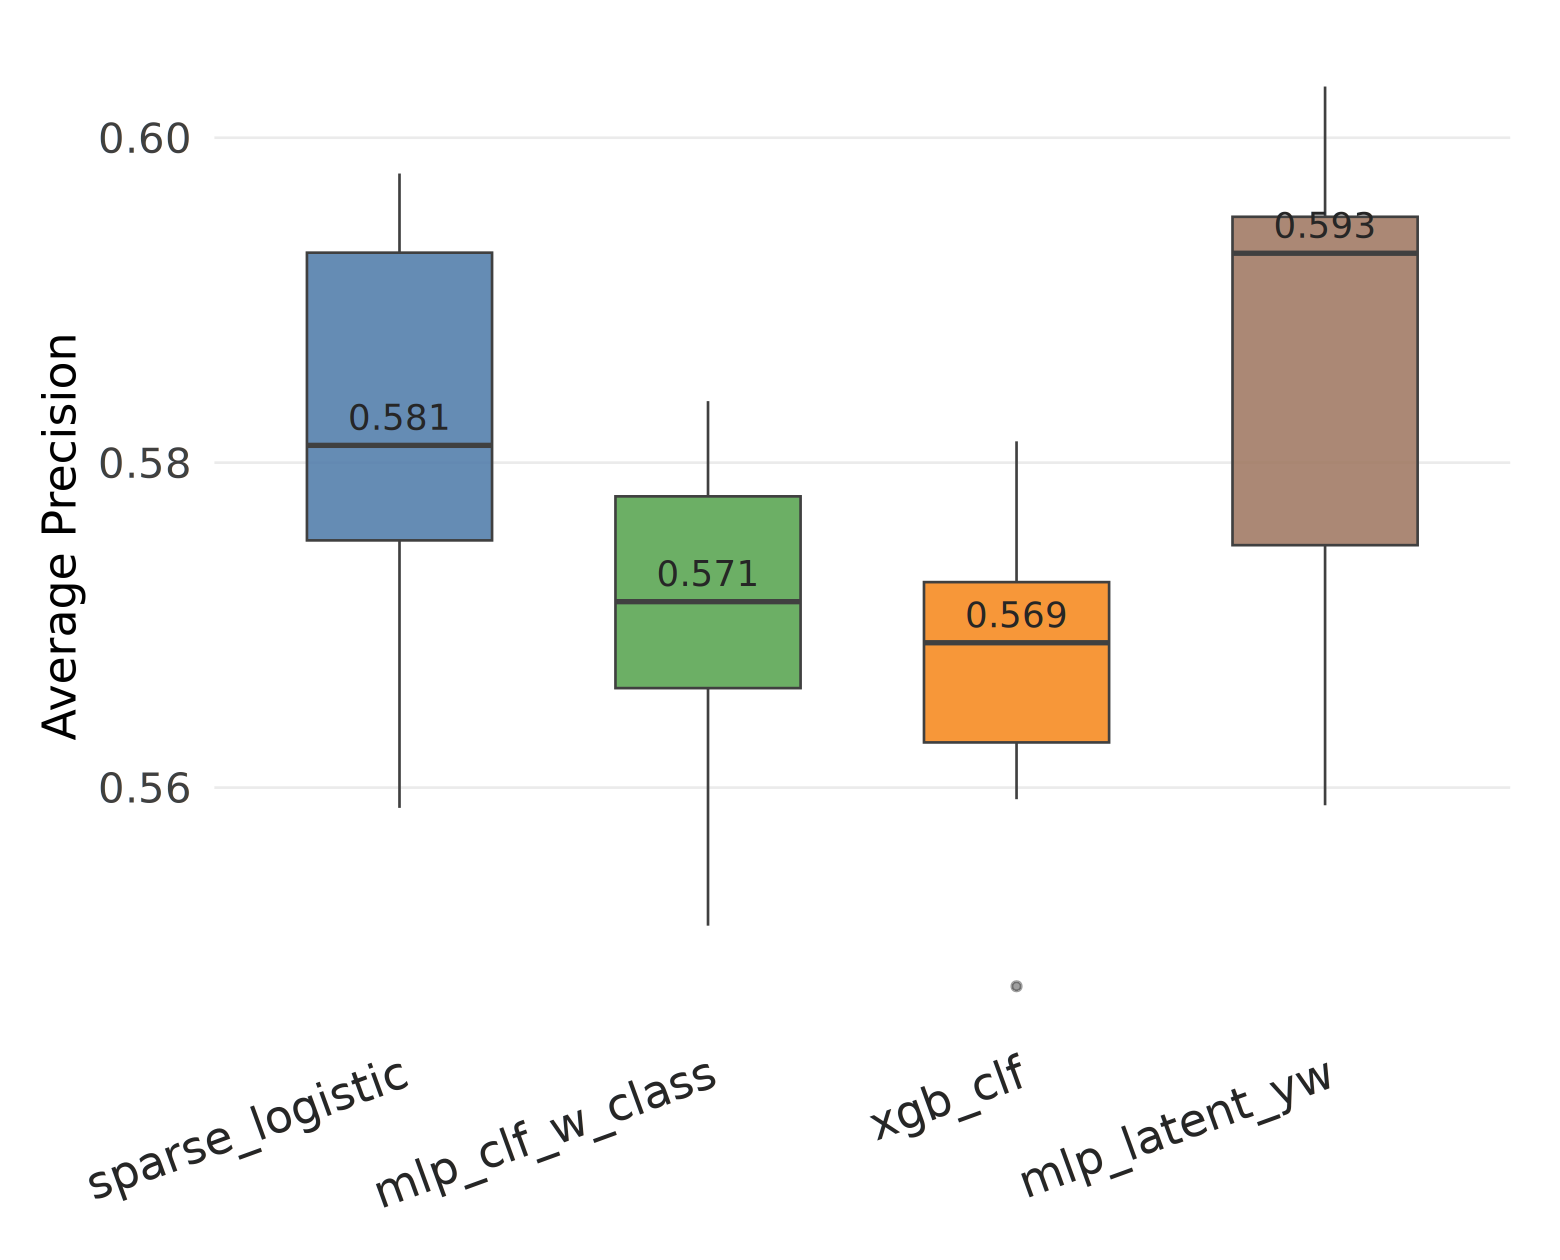
\includegraphics[width=\linewidth]{figures/fig_ap_w_class_ap_all_gvhd.png}
    \caption{GvHD}
  \end{subfigure}
  \caption{Test AP on the binarised selection probability, all models}
  \label{fig:ap-wcapa}
\end{figure}

\begin{figure}[H]
  \centering
  \begin{subfigure}[t]{0.32\textwidth}
    \centering
    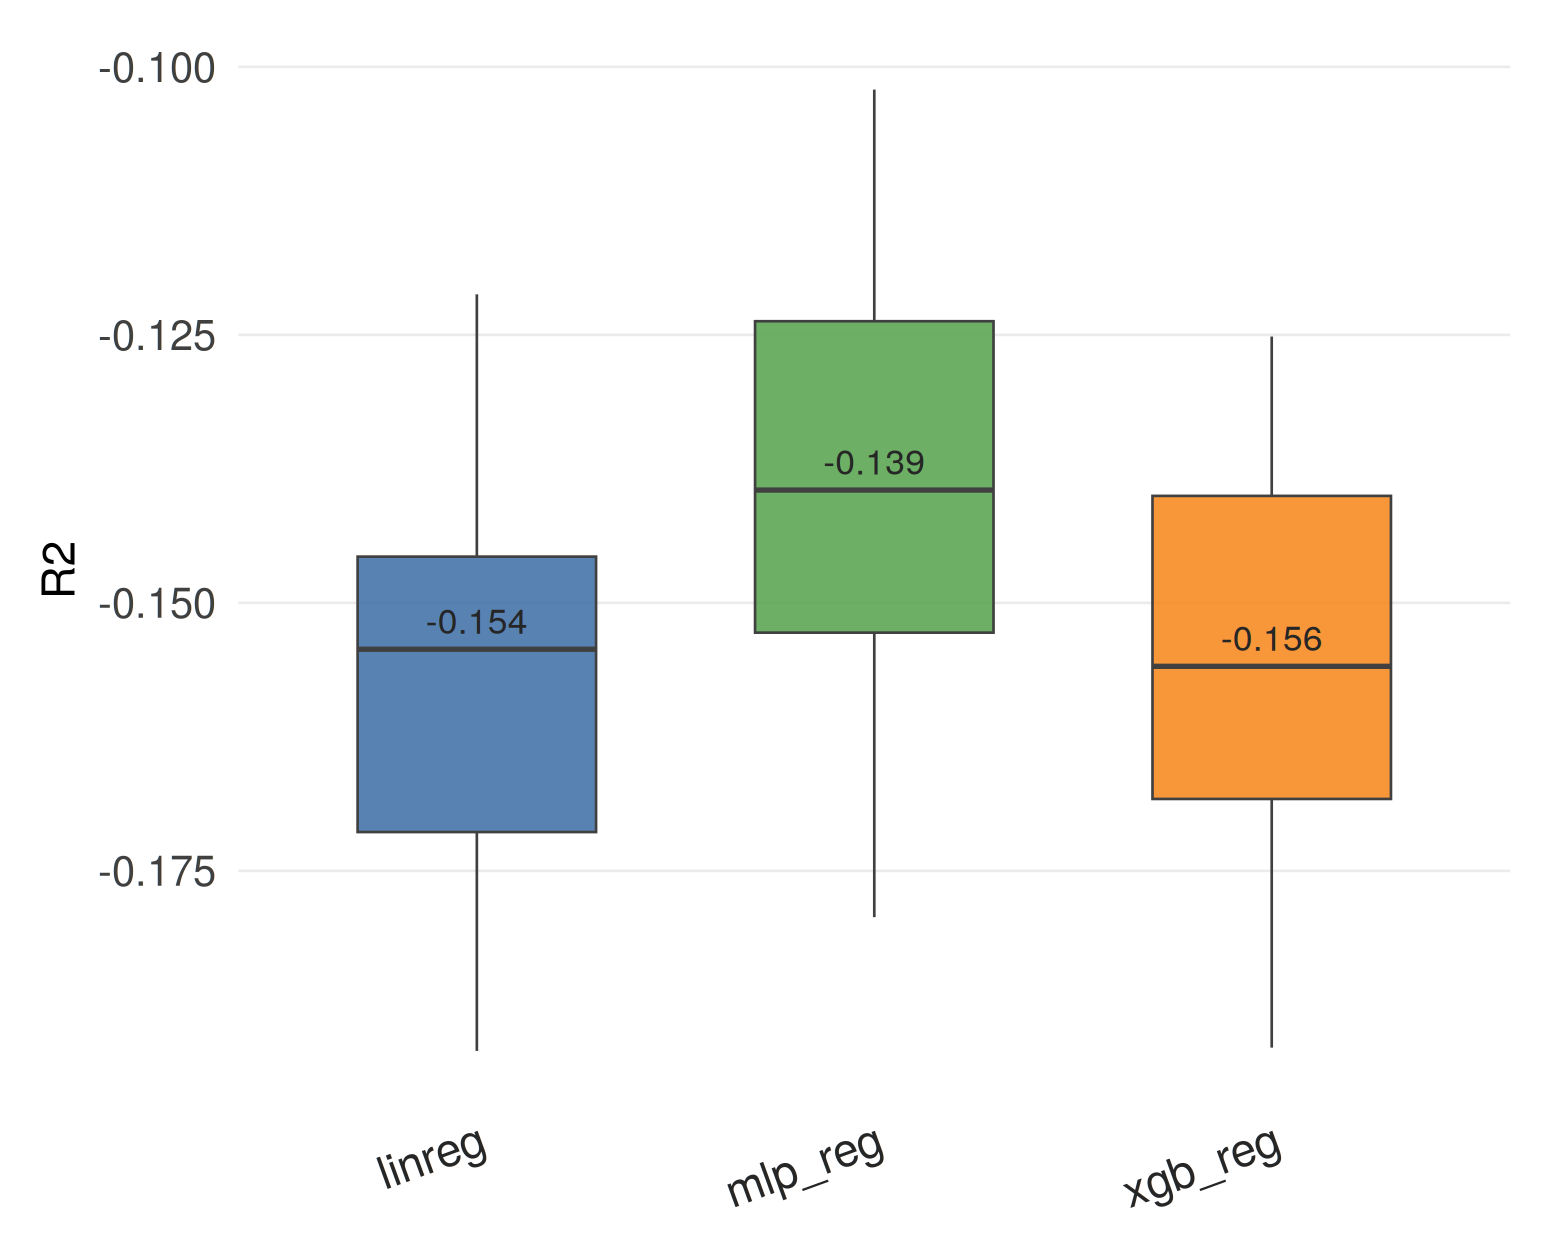
\includegraphics[width=\linewidth]{figures/fig_ap_w_reg_r2_baseline_crc.png}
    \caption{CRC}
  \end{subfigure}\hfill
  \begin{subfigure}[t]{0.32\textwidth}
    \centering
    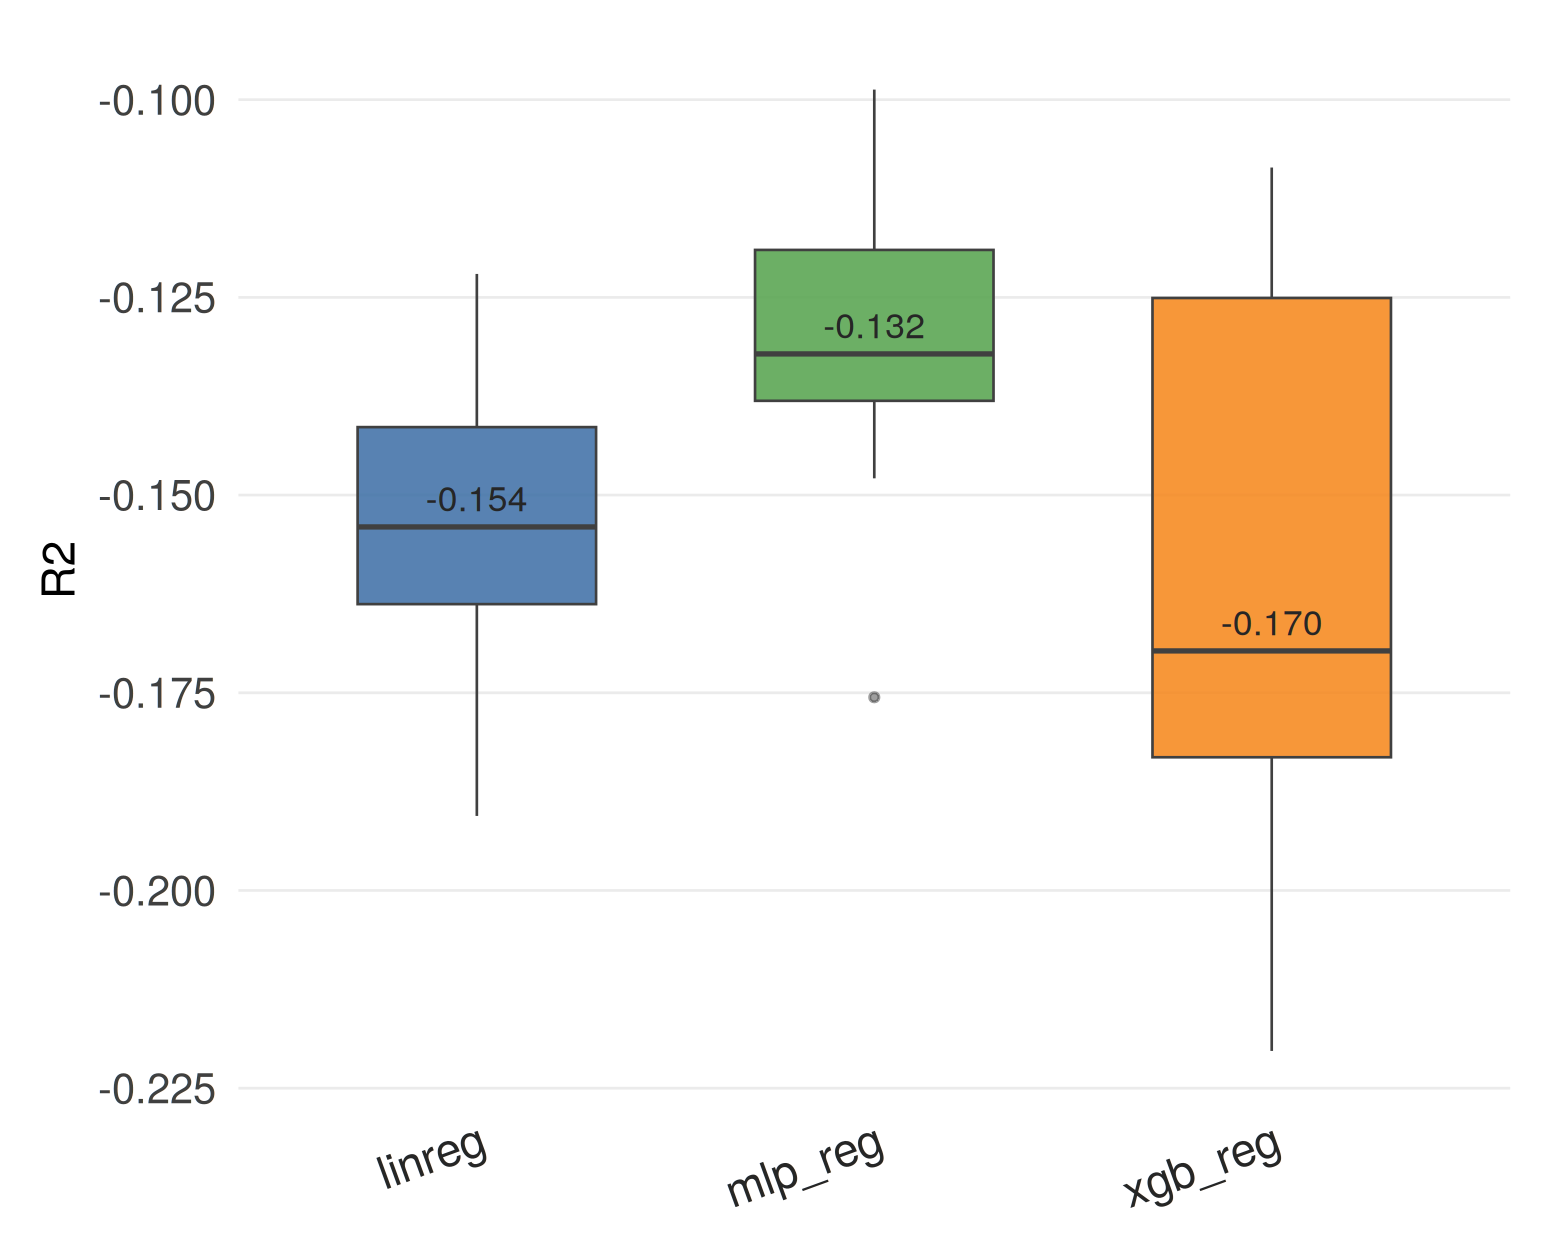
\includegraphics[width=\linewidth]{figures/fig_ap_w_reg_r2_baseline_ibd.png}
    \caption{IBD}
  \end{subfigure}\hfill
  \begin{subfigure}[t]{0.32\textwidth}
    \centering
    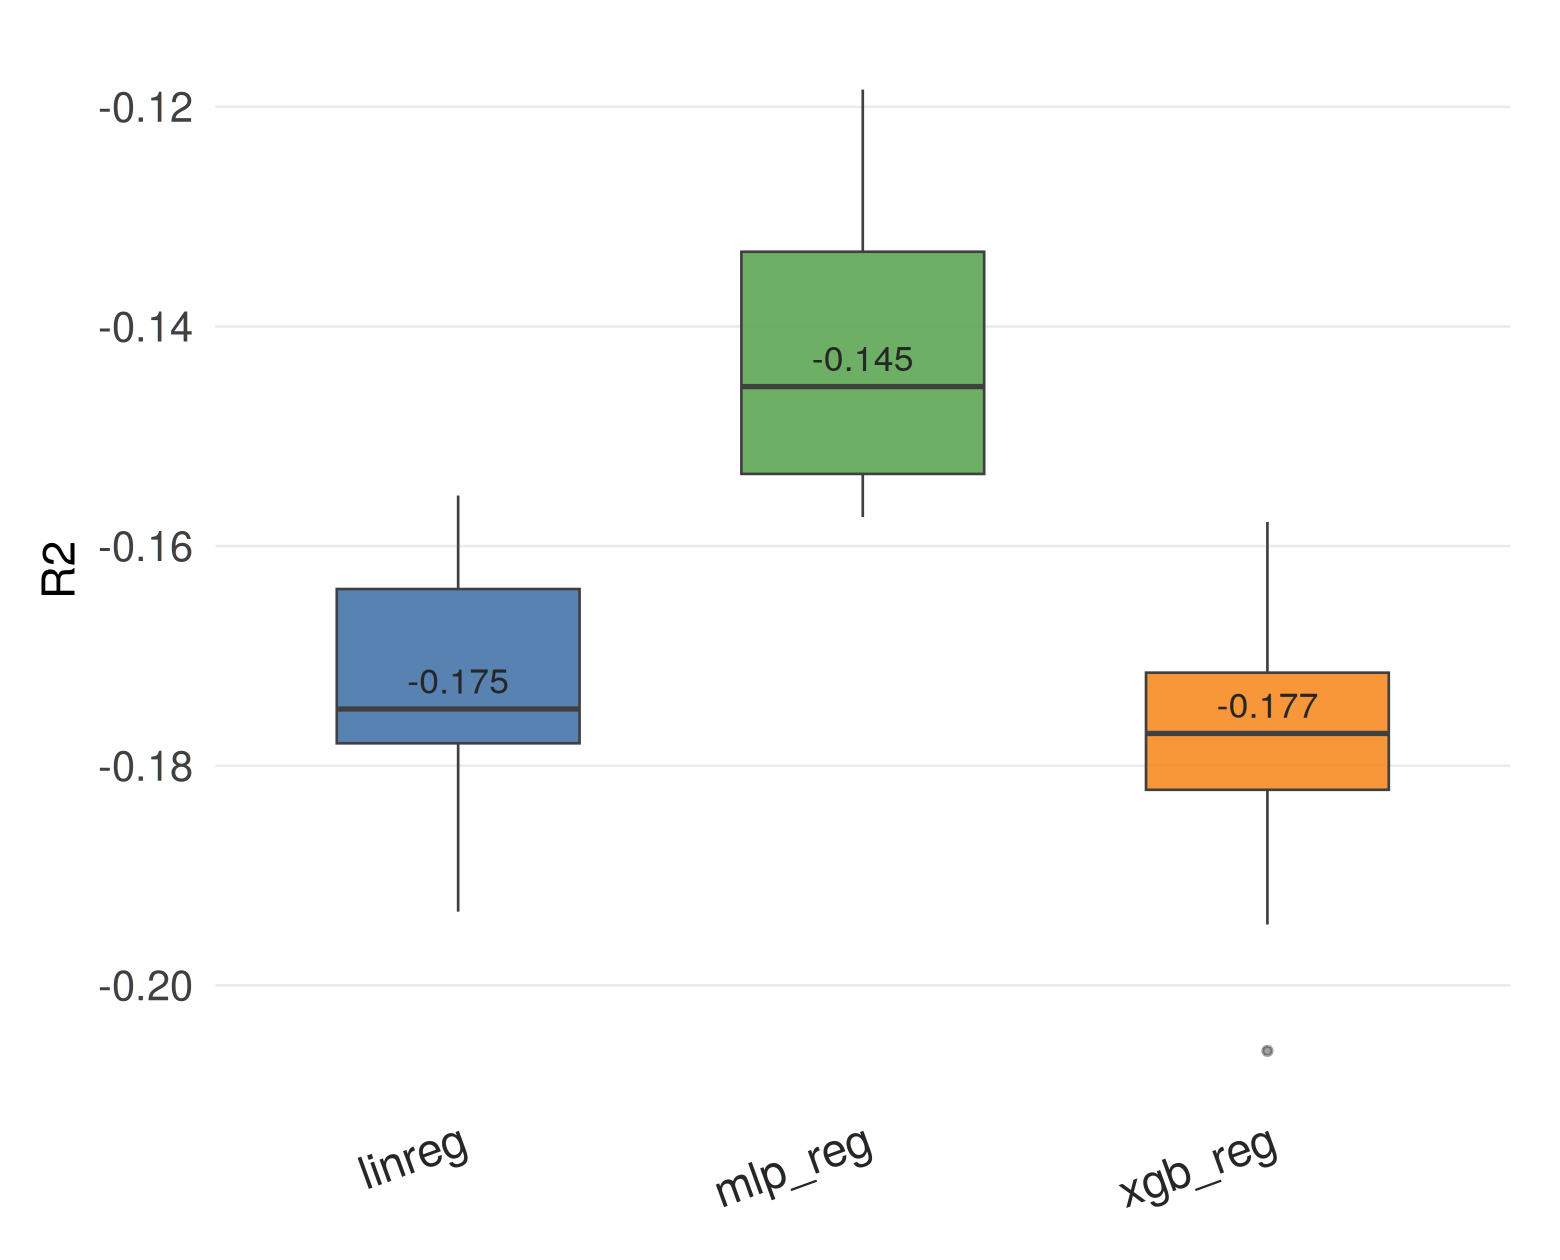
\includegraphics[width=\linewidth]{figures/fig_ap_w_reg_r2_baseline_gvhd.png}
    \caption{GvHD}
  \end{subfigure}
  \caption{Test $R^2$ on the edge selection probability, baseline models}
  \label{fig:ap-wrr2b}
\end{figure}

\begin{figure}[H]
  \centering
  \begin{subfigure}[t]{0.32\textwidth}
    \centering
    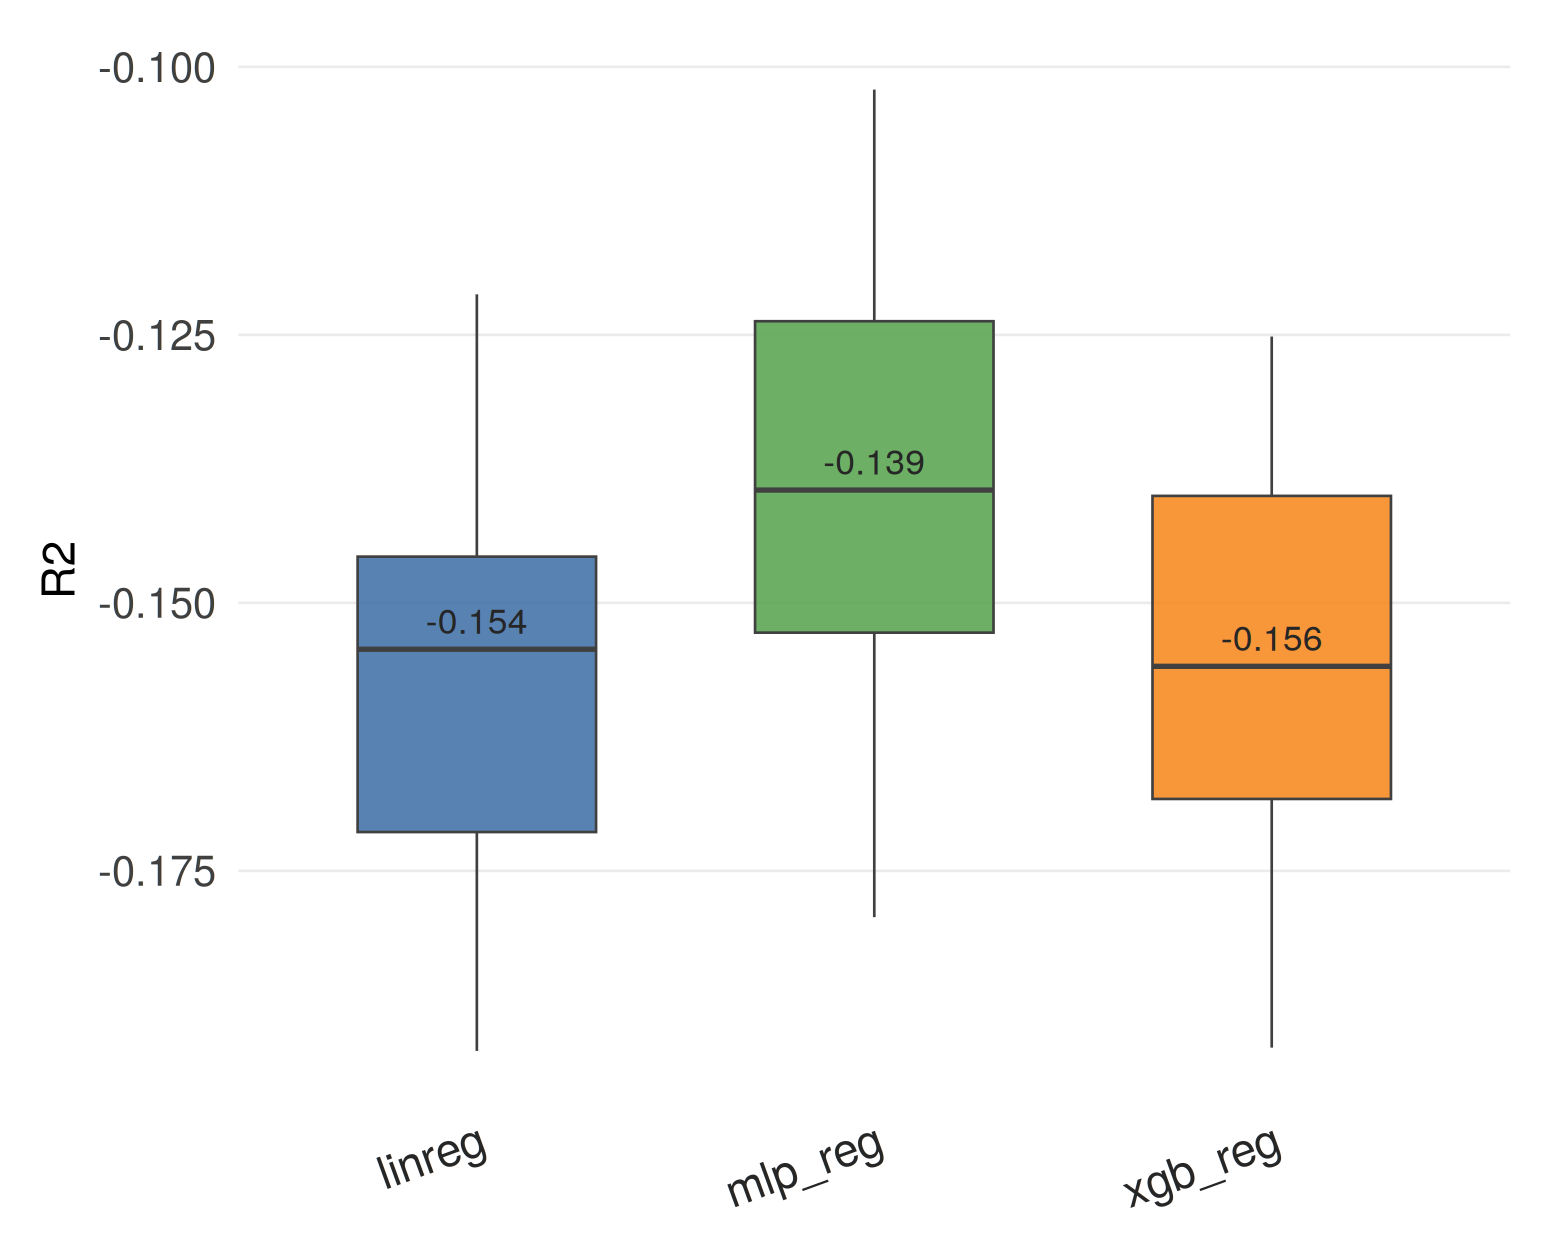
\includegraphics[width=\linewidth]{figures/fig_ap_w_reg_r2_all_crc.png}
    \caption{CRC}
  \end{subfigure}\hfill
  \begin{subfigure}[t]{0.32\textwidth}
    \centering
    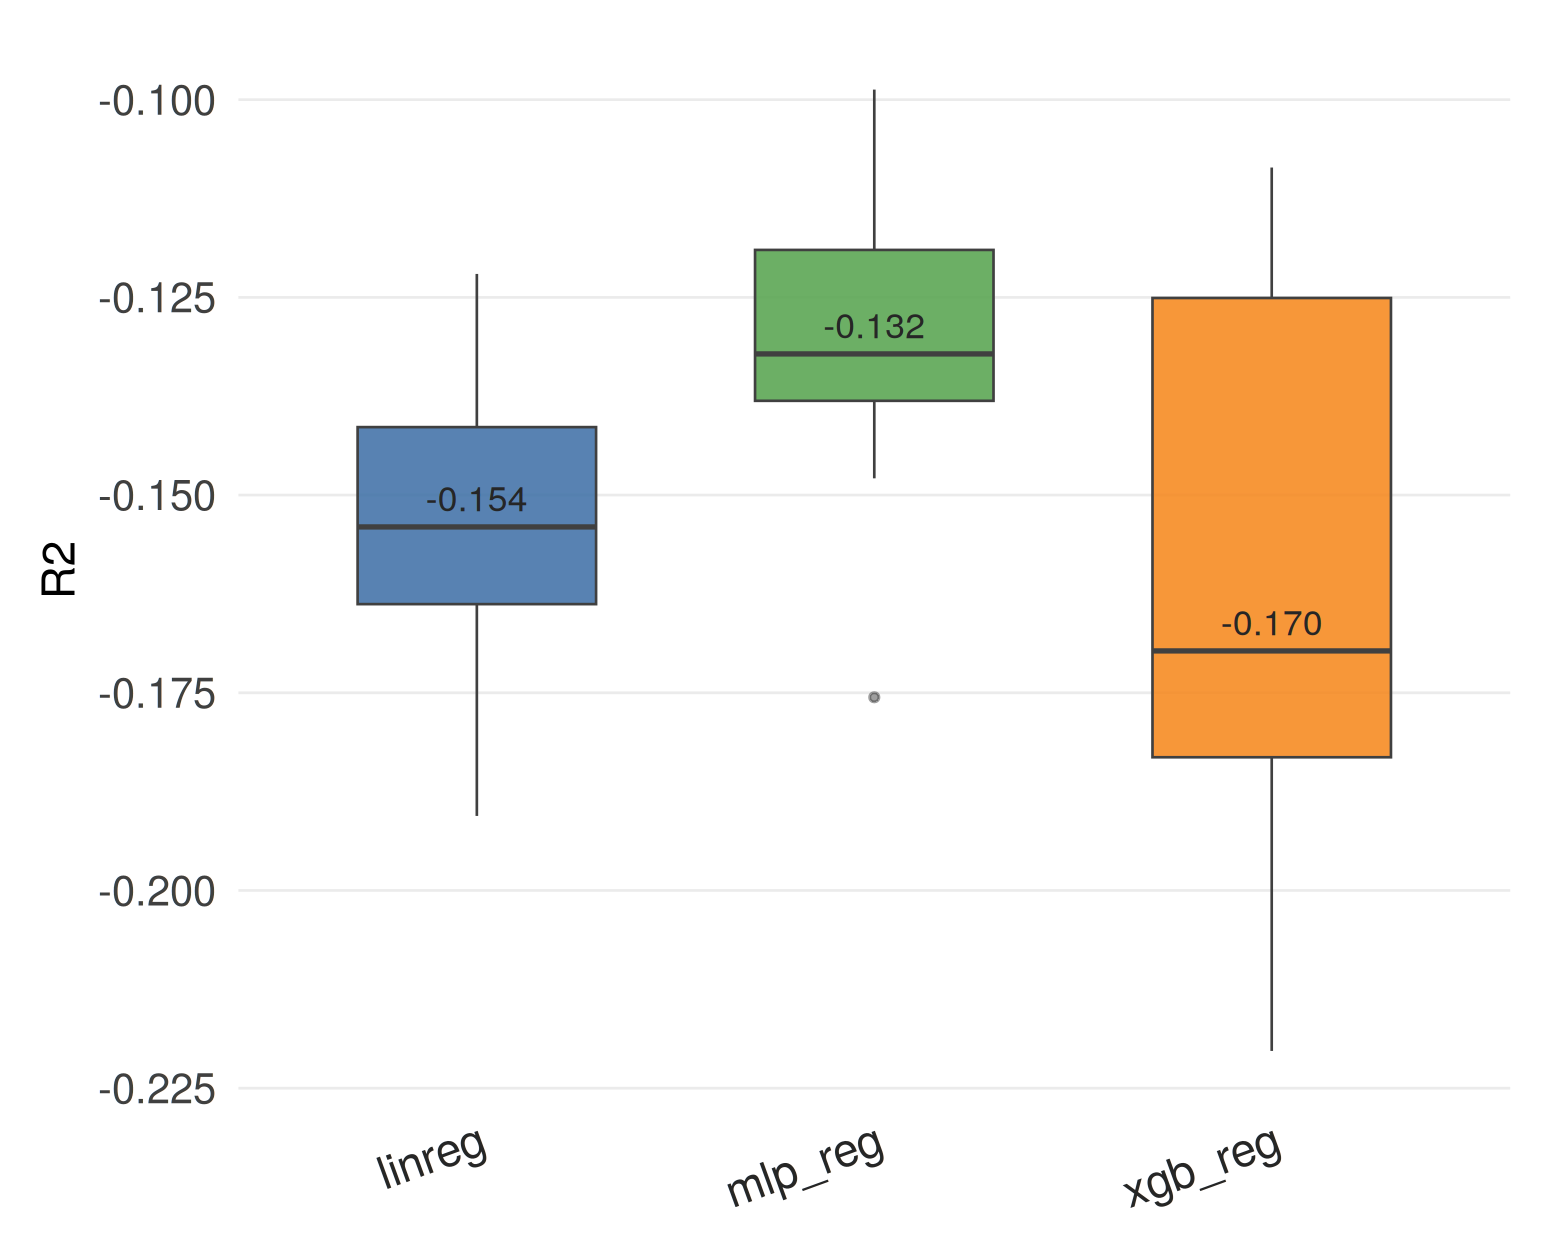
\includegraphics[width=\linewidth]{figures/fig_ap_w_reg_r2_all_ibd.png}
    \caption{IBD}
  \end{subfigure}\hfill
  \begin{subfigure}[t]{0.32\textwidth}
    \centering
    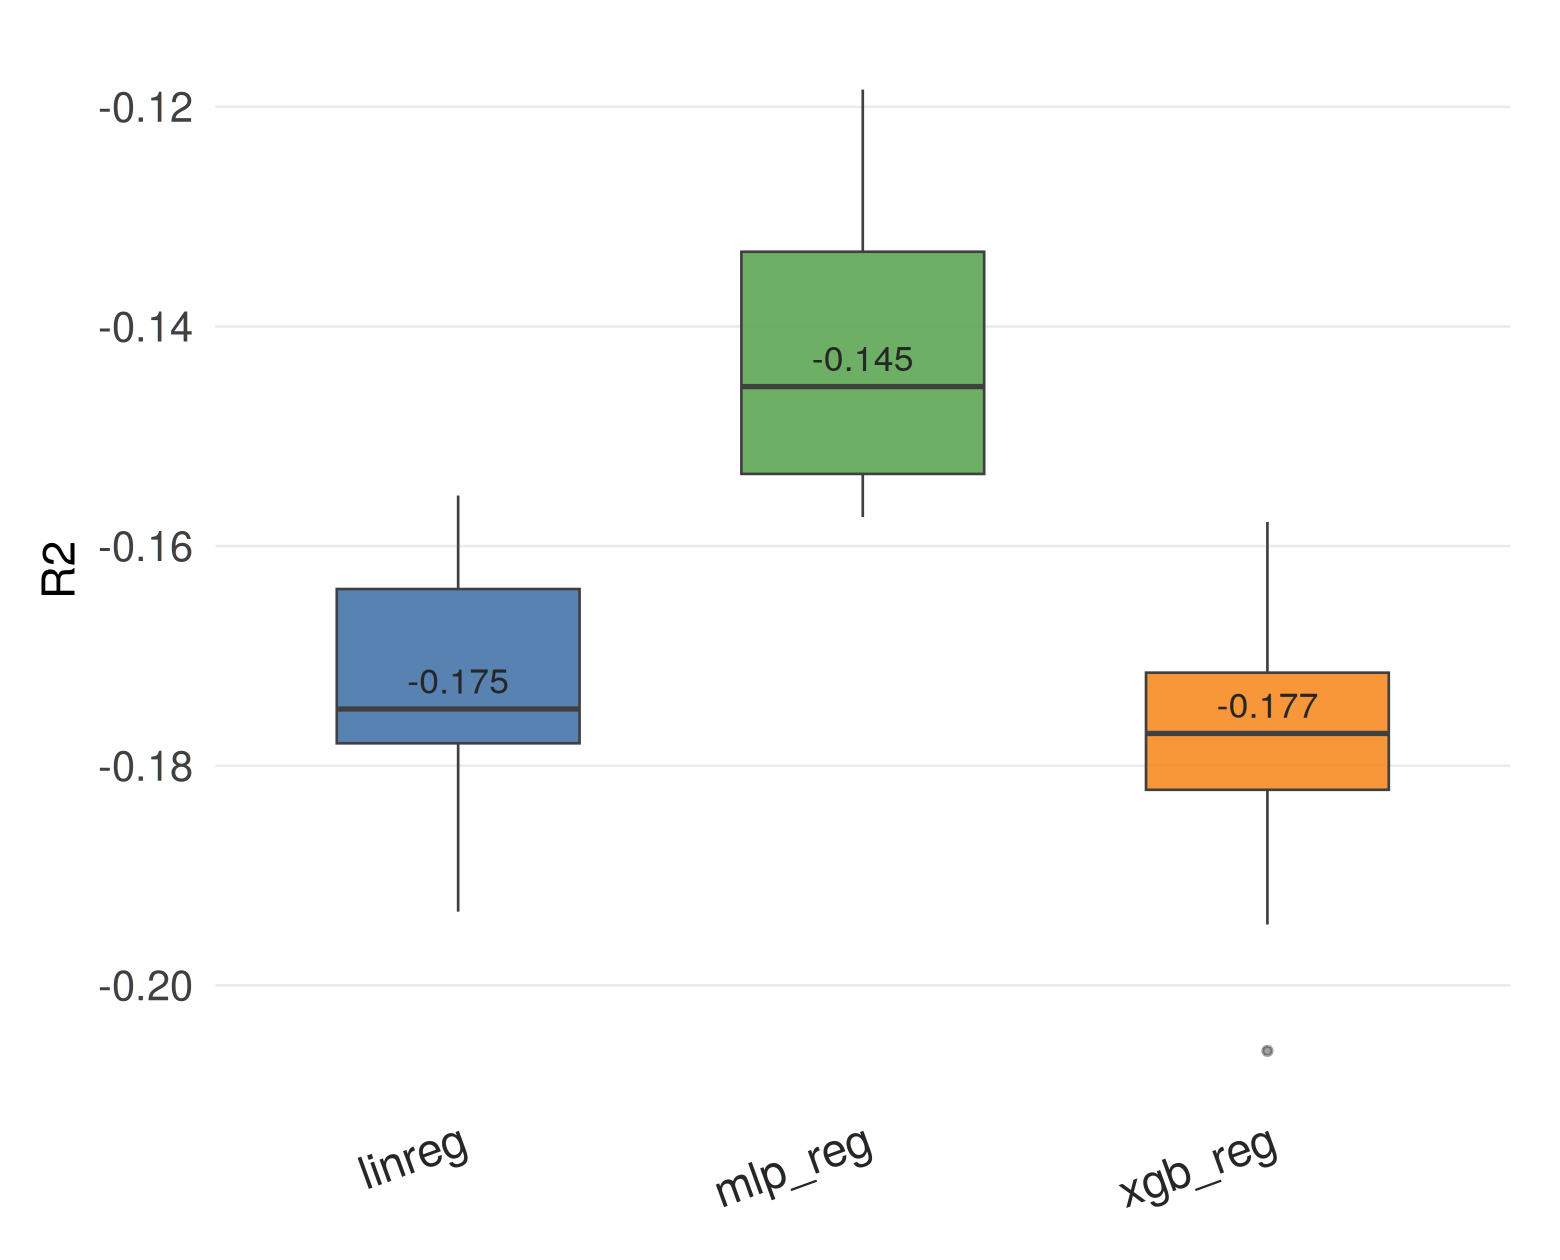
\includegraphics[width=\linewidth]{figures/fig_ap_w_reg_r2_all_gvhd.png}
    \caption{GvHD}
  \end{subfigure}
  \caption{Test $R^2$ on the edge selection probability, all models}
  \label{fig:ap-wrr2a}
\end{figure}

\subsection{Penalty Selection}

\begin{figure}[H]
  \centering
  \begin{subfigure}[t]{0.32\textwidth}
    \centering
    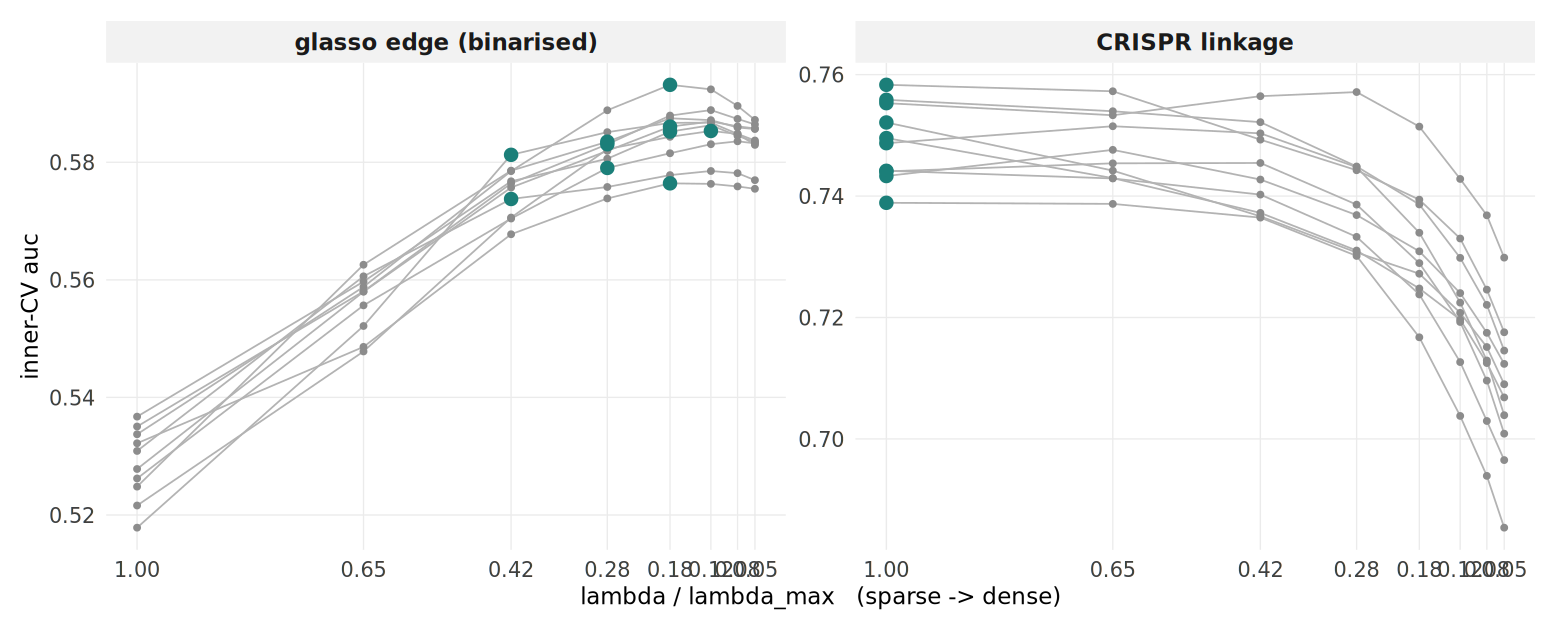
\includegraphics[width=\linewidth]{figures/fig_ap_lambda_cv_curve_crc.png}
    \caption{CRC}
  \end{subfigure}\hfill
  \begin{subfigure}[t]{0.32\textwidth}
    \centering
    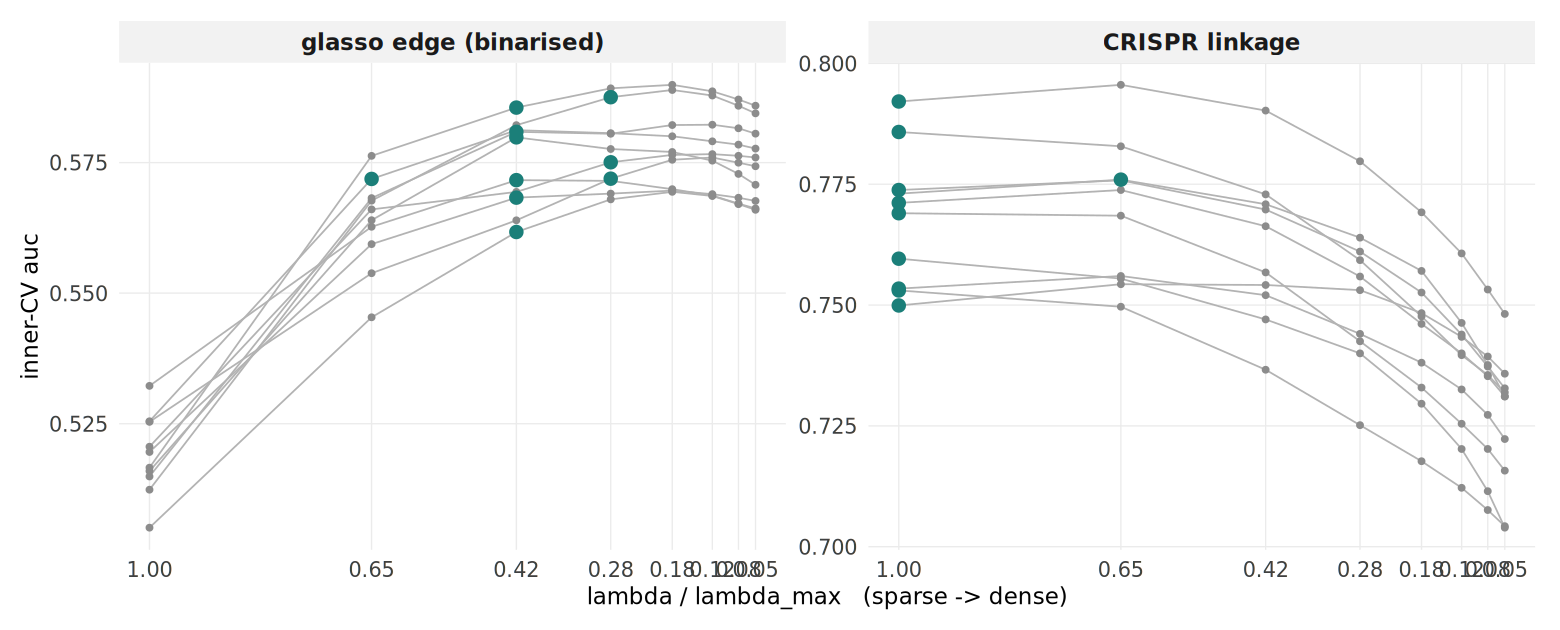
\includegraphics[width=\linewidth]{figures/fig_ap_lambda_cv_curve_ibd.png}
    \caption{IBD}
  \end{subfigure}\hfill
  \begin{subfigure}[t]{0.32\textwidth}
    \centering
    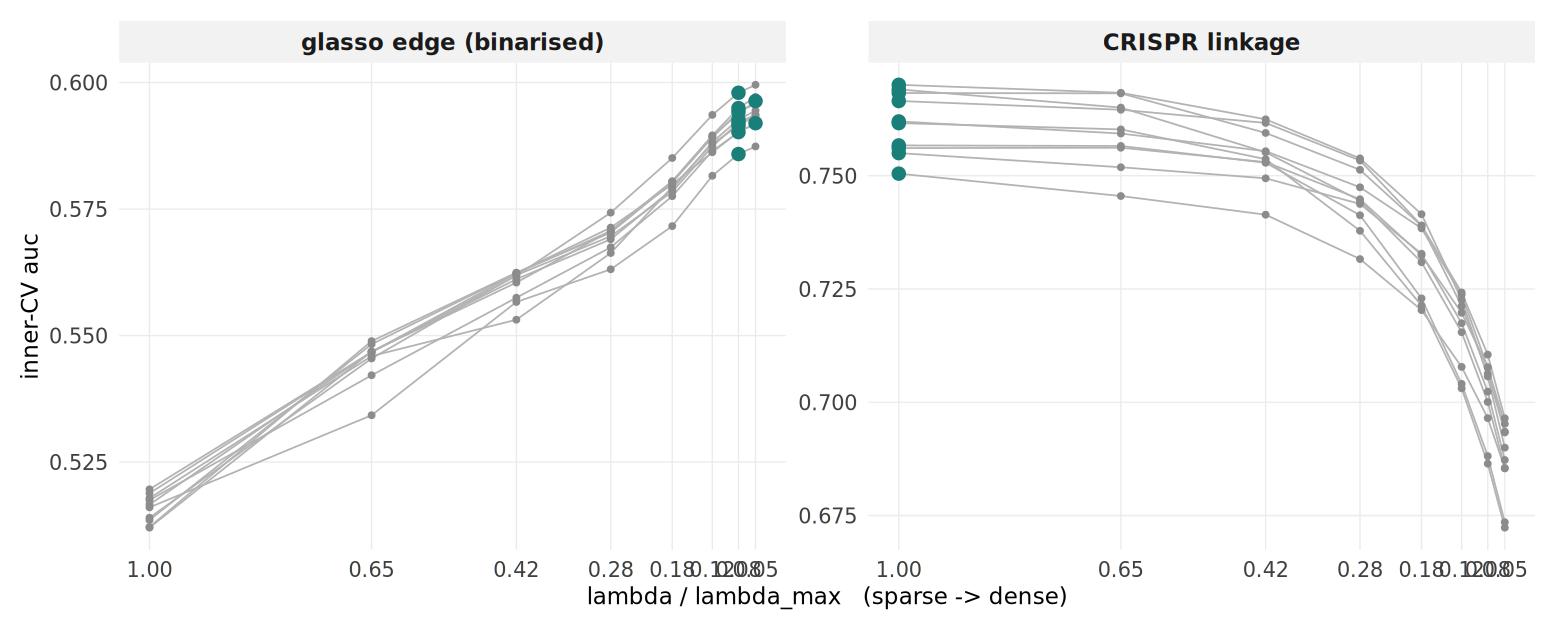
\includegraphics[width=\linewidth]{figures/fig_ap_lambda_cv_curve_gvhd.png}
    \caption{GvHD}
  \end{subfigure}
  \caption{Inner-CV score against the $L_1$ penalty, one line per outer fold}
  \label{fig:ap-lcurve}
\end{figure}

\begin{figure}[H]
  \centering
  \begin{subfigure}[t]{0.32\textwidth}
    \centering
    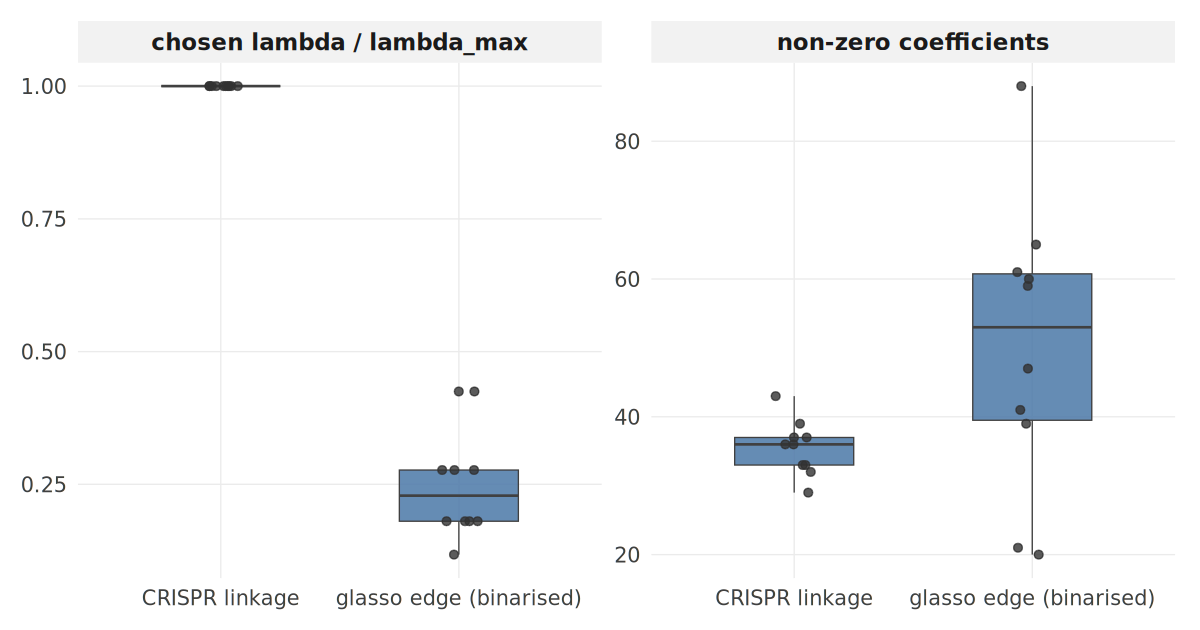
\includegraphics[width=\linewidth]{figures/fig_ap_lambda_cv_choice_crc.png}
    \caption{CRC}
  \end{subfigure}\hfill
  \begin{subfigure}[t]{0.32\textwidth}
    \centering
    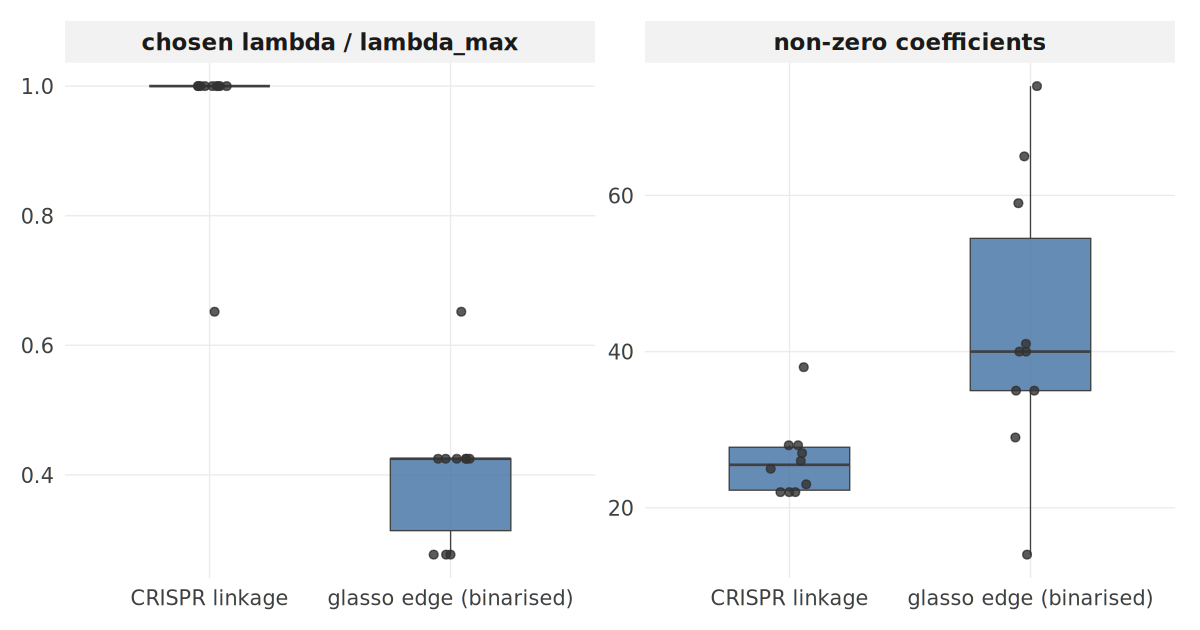
\includegraphics[width=\linewidth]{figures/fig_ap_lambda_cv_choice_ibd.png}
    \caption{IBD}
  \end{subfigure}\hfill
  \begin{subfigure}[t]{0.32\textwidth}
    \centering
    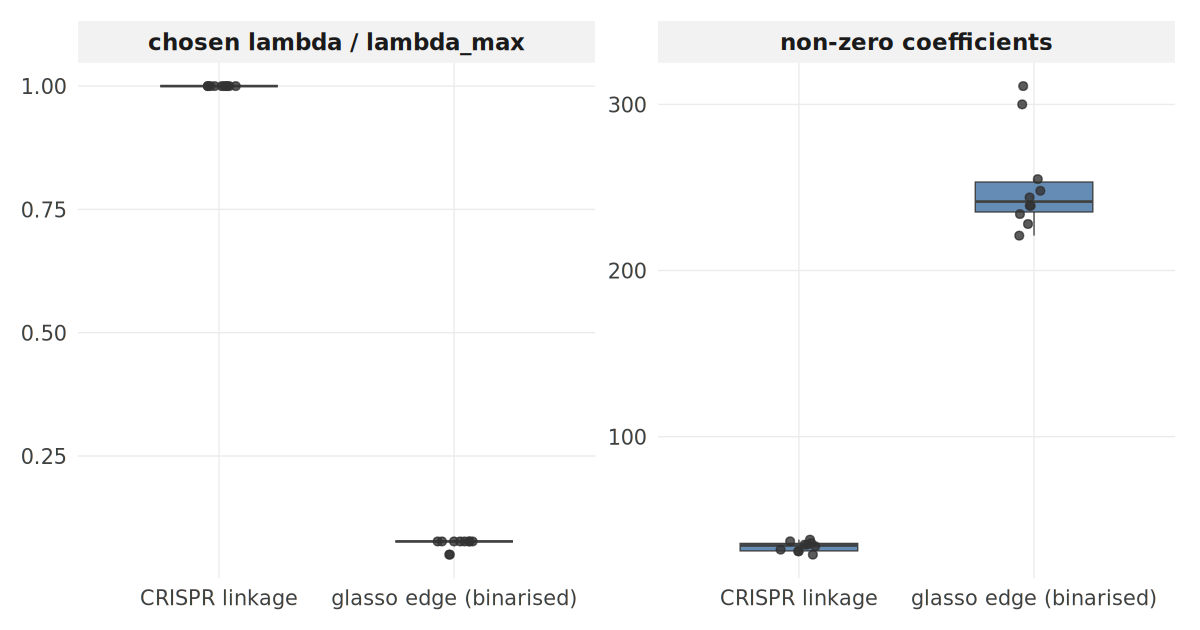
\includegraphics[width=\linewidth]{figures/fig_ap_lambda_cv_choice_gvhd.png}
    \caption{GvHD}
  \end{subfigure}
  \caption{Selected penalty ratio and resulting support size}
  \label{fig:ap-lchoice}
\end{figure}

\subsection{Binarisation Threshold}

\begin{figure}[H]
  \centering
  \begin{subfigure}[t]{0.32\textwidth}
    \centering
    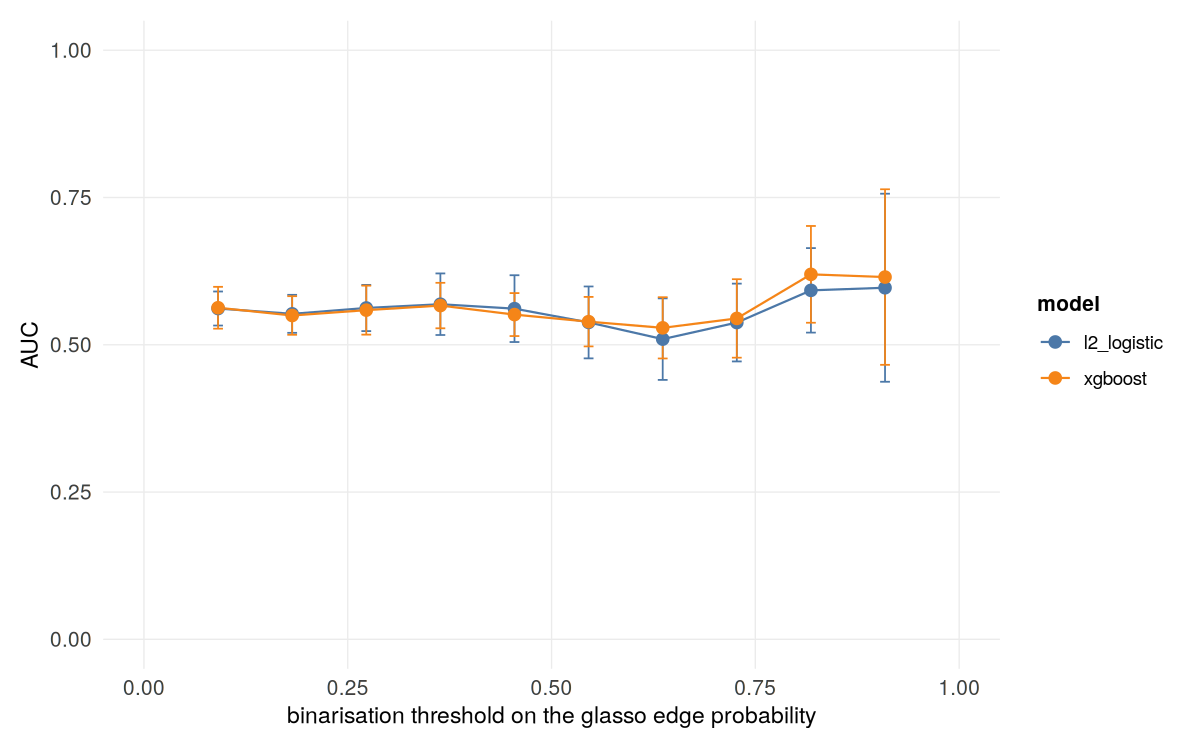
\includegraphics[width=\linewidth]{figures/fig_wthreshold_crc.png}
    \caption{CRC}
  \end{subfigure}\hfill
  \begin{subfigure}[t]{0.32\textwidth}
    \centering
    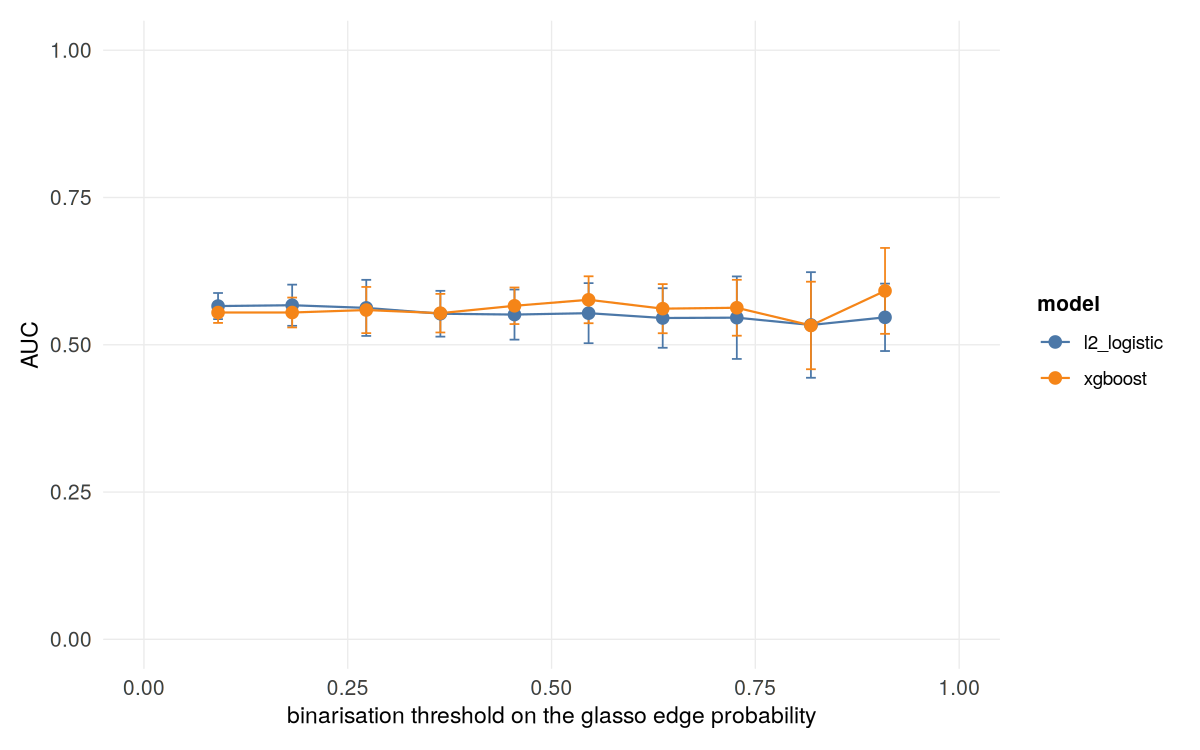
\includegraphics[width=\linewidth]{figures/fig_wthreshold_ibd.png}
    \caption{IBD}
  \end{subfigure}\hfill
  \begin{subfigure}[t]{0.32\textwidth}
    \centering
    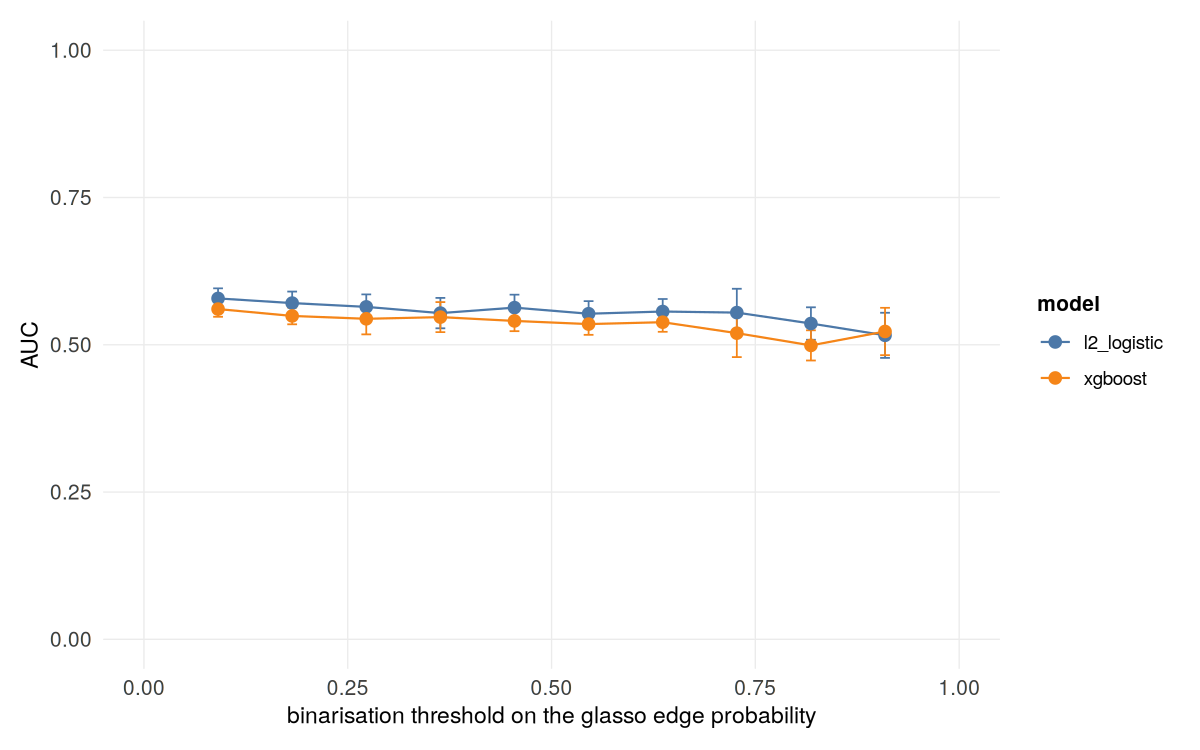
\includegraphics[width=\linewidth]{figures/fig_wthreshold_gvhd.png}
    \caption{GvHD}
  \end{subfigure}
  \caption{Test AUC against the binarisation threshold \(\tau\)}
  \label{fig:ap-wthreshold}
\end{figure}

\subsection{Stability Selection}

\begin{figure}[H]
  \centering
  \begin{subfigure}[t]{0.32\textwidth}
    \centering
    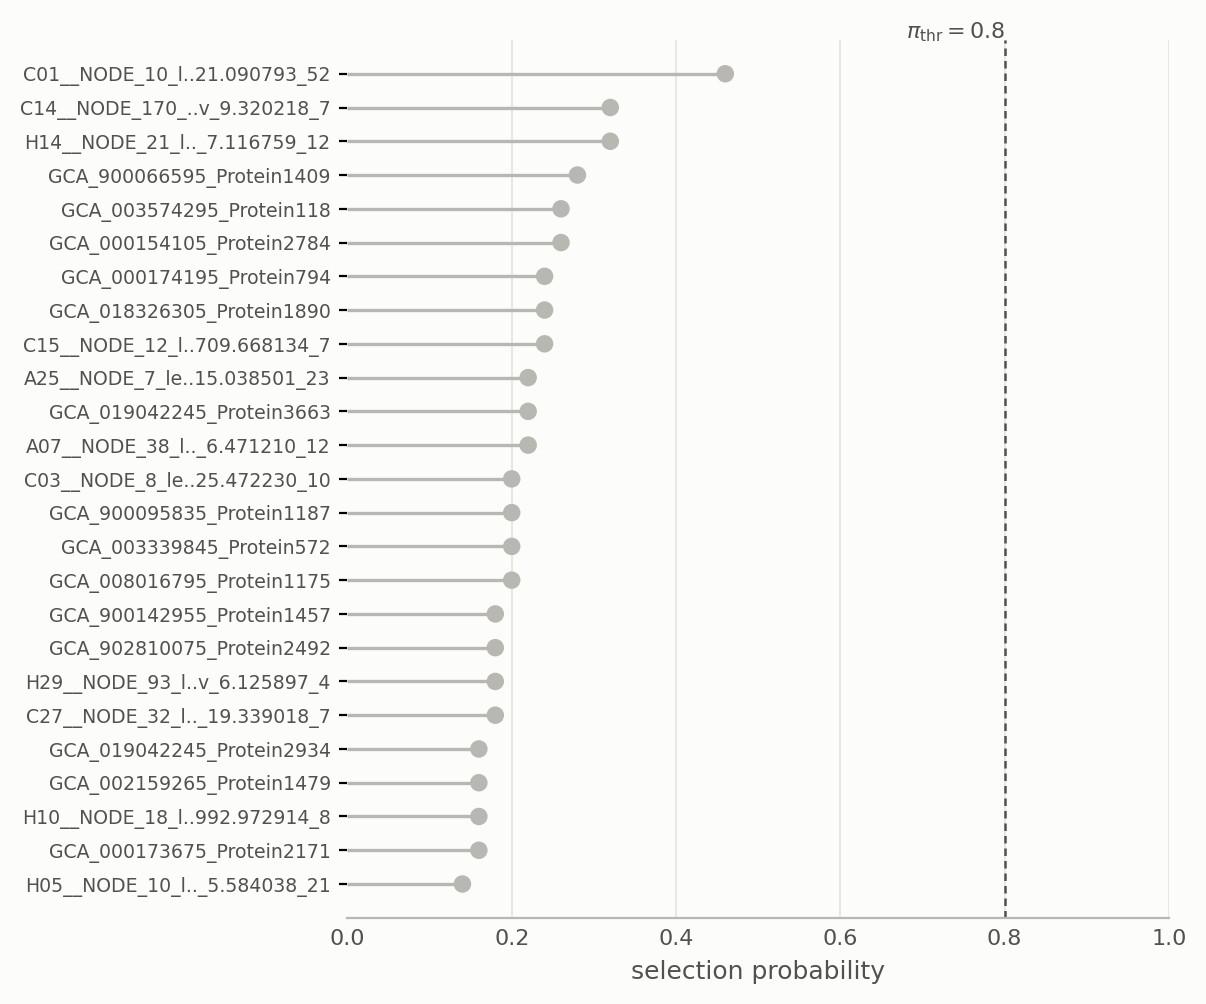
\includegraphics[width=\linewidth]{figures/fig_stability_crc.png}
    \caption{CRC}
  \end{subfigure}\hfill
  \begin{subfigure}[t]{0.32\textwidth}
    \centering
    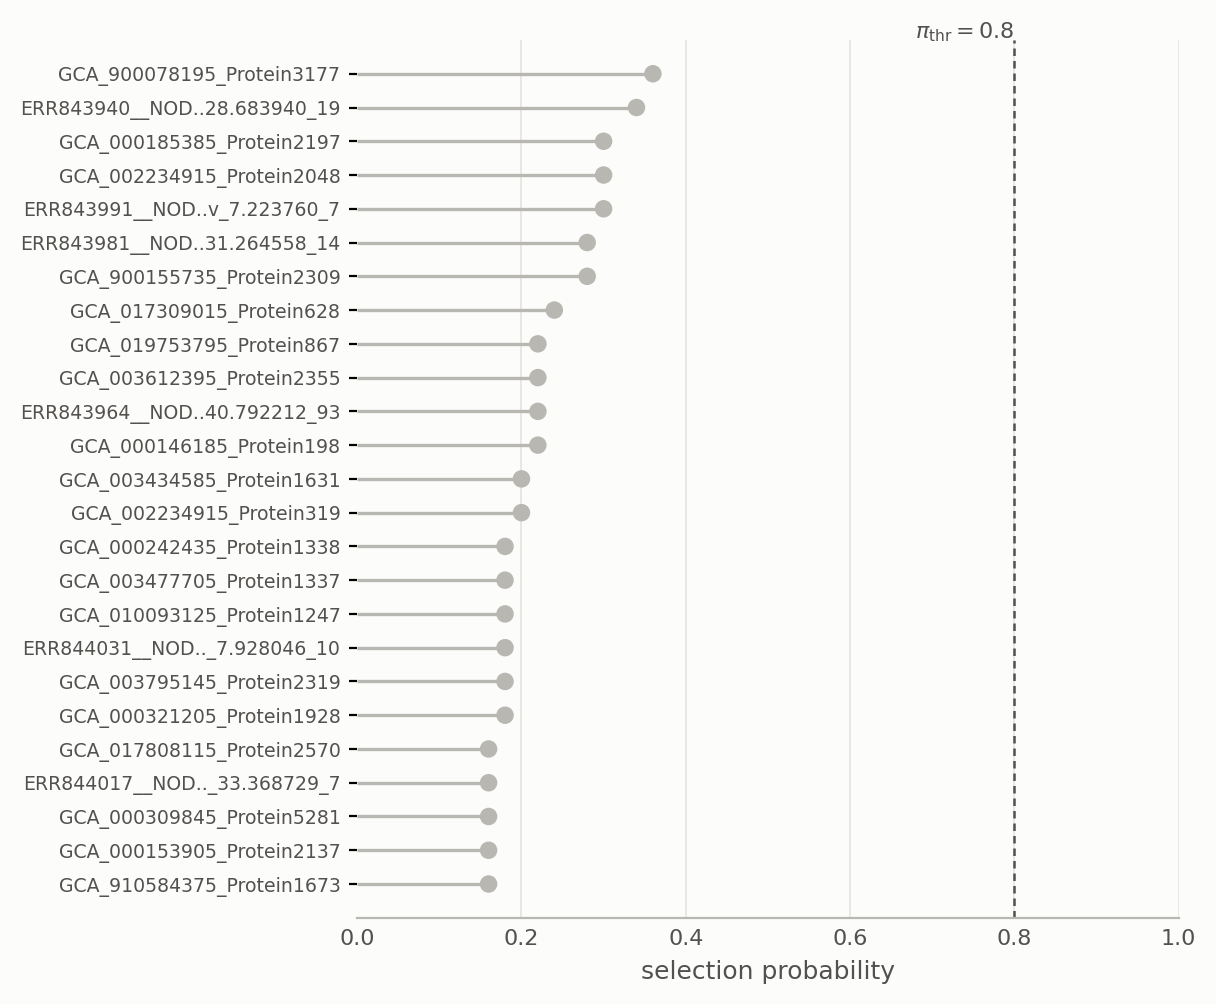
\includegraphics[width=\linewidth]{figures/fig_stability_ibd.png}
    \caption{IBD}
  \end{subfigure}\hfill
  \begin{subfigure}[t]{0.32\textwidth}
    \centering
    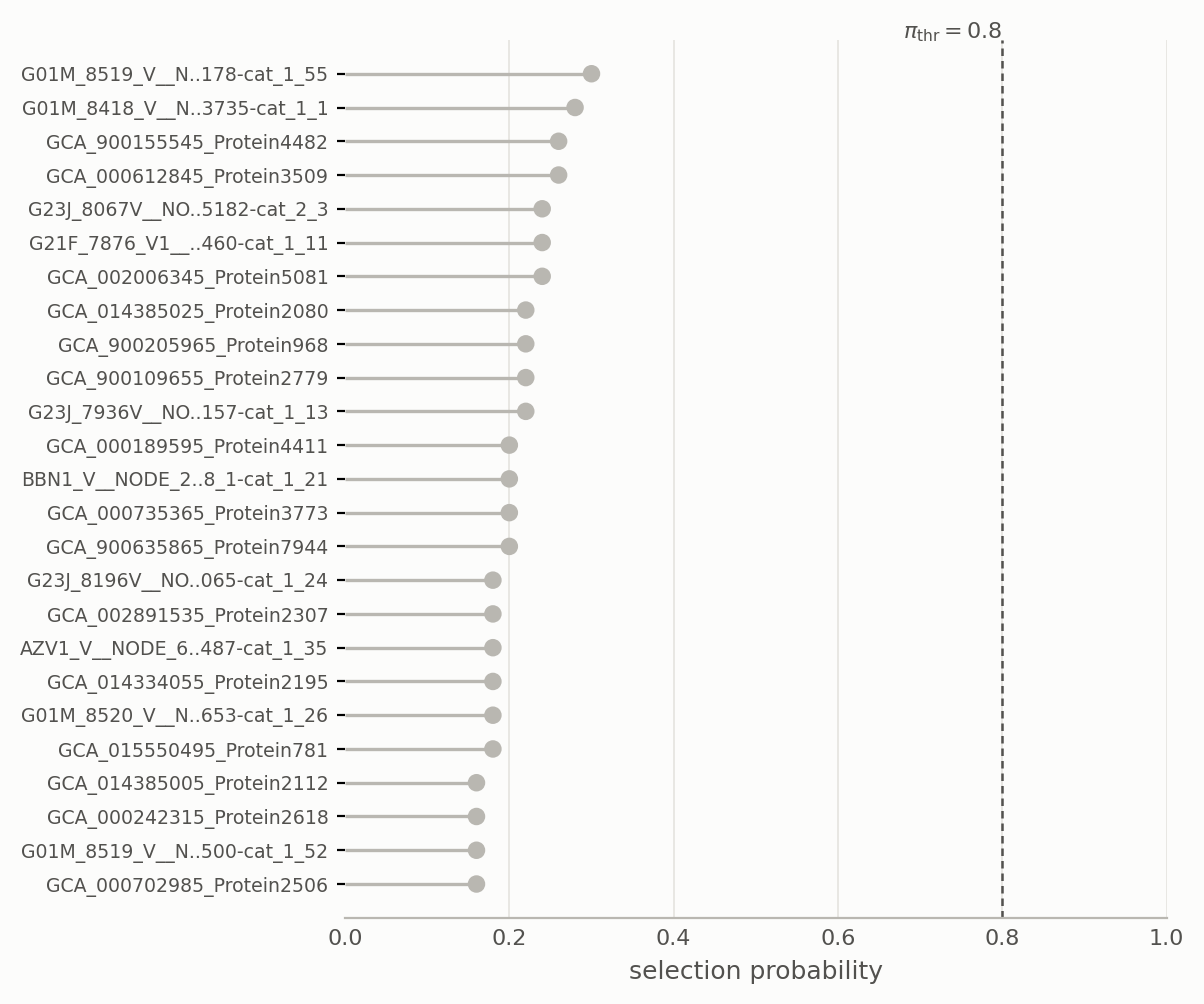
\includegraphics[width=\linewidth]{figures/fig_stability_gvhd.png}
    \caption{GvHD}
  \end{subfigure}
  \caption{Selection probabilities of the 25 highest-ranked protein clusters, with the threshold
  \(\pi_{\mathrm{thr}}=0.8\) marked}
  \label{fig:ap-stab}
\end{figure}
